\documentclass[11pt,]{report}
\usepackage{lmodern}
\usepackage{amssymb,amsmath}
\usepackage{ifxetex,ifluatex}
\usepackage{fixltx2e} % provides \textsubscript
\ifnum 0\ifxetex 1\fi\ifluatex 1\fi=0 % if pdftex
  \usepackage[T1]{fontenc}
  \usepackage[utf8]{inputenc}
\else % if luatex or xelatex
  \ifxetex
    \usepackage{mathspec}
  \else
    \usepackage{fontspec}
  \fi
  \defaultfontfeatures{Ligatures=TeX,Scale=MatchLowercase}
\fi
% use upquote if available, for straight quotes in verbatim environments
\IfFileExists{upquote.sty}{\usepackage{upquote}}{}
% use microtype if available
\IfFileExists{microtype.sty}{%
\usepackage{microtype}
\UseMicrotypeSet[protrusion]{basicmath} % disable protrusion for tt fonts
}{}
\usepackage[left=3cm, right=3cm, top=3cm]{geometry}
\usepackage{hyperref}
\PassOptionsToPackage{usenames,dvipsnames}{color} % color is loaded by hyperref
\hypersetup{unicode=true,
            colorlinks=true,
            linkcolor=black,
            citecolor=Blue,
            urlcolor=blue,
            breaklinks=true}
\urlstyle{same}  % don't use monospace font for urls
\usepackage{color}
\usepackage{fancyvrb}
\newcommand{\VerbBar}{|}
\newcommand{\VERB}{\Verb[commandchars=\\\{\}]}
\DefineVerbatimEnvironment{Highlighting}{Verbatim}{commandchars=\\\{\}}
% Add ',fontsize=\small' for more characters per line
\usepackage{framed}
\definecolor{shadecolor}{RGB}{248,248,248}
\newenvironment{Shaded}{\begin{snugshade}}{\end{snugshade}}
\newcommand{\KeywordTok}[1]{\textcolor[rgb]{0.13,0.29,0.53}{\textbf{#1}}}
\newcommand{\DataTypeTok}[1]{\textcolor[rgb]{0.13,0.29,0.53}{#1}}
\newcommand{\DecValTok}[1]{\textcolor[rgb]{0.00,0.00,0.81}{#1}}
\newcommand{\BaseNTok}[1]{\textcolor[rgb]{0.00,0.00,0.81}{#1}}
\newcommand{\FloatTok}[1]{\textcolor[rgb]{0.00,0.00,0.81}{#1}}
\newcommand{\ConstantTok}[1]{\textcolor[rgb]{0.00,0.00,0.00}{#1}}
\newcommand{\CharTok}[1]{\textcolor[rgb]{0.31,0.60,0.02}{#1}}
\newcommand{\SpecialCharTok}[1]{\textcolor[rgb]{0.00,0.00,0.00}{#1}}
\newcommand{\StringTok}[1]{\textcolor[rgb]{0.31,0.60,0.02}{#1}}
\newcommand{\VerbatimStringTok}[1]{\textcolor[rgb]{0.31,0.60,0.02}{#1}}
\newcommand{\SpecialStringTok}[1]{\textcolor[rgb]{0.31,0.60,0.02}{#1}}
\newcommand{\ImportTok}[1]{#1}
\newcommand{\CommentTok}[1]{\textcolor[rgb]{0.56,0.35,0.01}{\textit{#1}}}
\newcommand{\DocumentationTok}[1]{\textcolor[rgb]{0.56,0.35,0.01}{\textbf{\textit{#1}}}}
\newcommand{\AnnotationTok}[1]{\textcolor[rgb]{0.56,0.35,0.01}{\textbf{\textit{#1}}}}
\newcommand{\CommentVarTok}[1]{\textcolor[rgb]{0.56,0.35,0.01}{\textbf{\textit{#1}}}}
\newcommand{\OtherTok}[1]{\textcolor[rgb]{0.56,0.35,0.01}{#1}}
\newcommand{\FunctionTok}[1]{\textcolor[rgb]{0.00,0.00,0.00}{#1}}
\newcommand{\VariableTok}[1]{\textcolor[rgb]{0.00,0.00,0.00}{#1}}
\newcommand{\ControlFlowTok}[1]{\textcolor[rgb]{0.13,0.29,0.53}{\textbf{#1}}}
\newcommand{\OperatorTok}[1]{\textcolor[rgb]{0.81,0.36,0.00}{\textbf{#1}}}
\newcommand{\BuiltInTok}[1]{#1}
\newcommand{\ExtensionTok}[1]{#1}
\newcommand{\PreprocessorTok}[1]{\textcolor[rgb]{0.56,0.35,0.01}{\textit{#1}}}
\newcommand{\AttributeTok}[1]{\textcolor[rgb]{0.77,0.63,0.00}{#1}}
\newcommand{\RegionMarkerTok}[1]{#1}
\newcommand{\InformationTok}[1]{\textcolor[rgb]{0.56,0.35,0.01}{\textbf{\textit{#1}}}}
\newcommand{\WarningTok}[1]{\textcolor[rgb]{0.56,0.35,0.01}{\textbf{\textit{#1}}}}
\newcommand{\AlertTok}[1]{\textcolor[rgb]{0.94,0.16,0.16}{#1}}
\newcommand{\ErrorTok}[1]{\textcolor[rgb]{0.64,0.00,0.00}{\textbf{#1}}}
\newcommand{\NormalTok}[1]{#1}
\usepackage{longtable,booktabs}
\usepackage{graphicx,grffile}
\makeatletter
\def\maxwidth{\ifdim\Gin@nat@width>\linewidth\linewidth\else\Gin@nat@width\fi}
\def\maxheight{\ifdim\Gin@nat@height>\textheight\textheight\else\Gin@nat@height\fi}
\makeatother
% Scale images if necessary, so that they will not overflow the page
% margins by default, and it is still possible to overwrite the defaults
% using explicit options in \includegraphics[width, height, ...]{}
\setkeys{Gin}{width=\maxwidth,height=\maxheight,keepaspectratio}
\IfFileExists{parskip.sty}{%
\usepackage{parskip}
}{% else
\setlength{\parindent}{0pt}
\setlength{\parskip}{6pt plus 2pt minus 1pt}
}
\setlength{\emergencystretch}{3em}  % prevent overfull lines
\providecommand{\tightlist}{%
  \setlength{\itemsep}{0pt}\setlength{\parskip}{0pt}}
\setcounter{secnumdepth}{5}
% Redefines (sub)paragraphs to behave more like sections
\ifx\paragraph\undefined\else
\let\oldparagraph\paragraph
\renewcommand{\paragraph}[1]{\oldparagraph{#1}\mbox{}}
\fi
\ifx\subparagraph\undefined\else
\let\oldsubparagraph\subparagraph
\renewcommand{\subparagraph}[1]{\oldsubparagraph{#1}\mbox{}}
\fi

%%% Use protect on footnotes to avoid problems with footnotes in titles
\let\rmarkdownfootnote\footnote%
\def\footnote{\protect\rmarkdownfootnote}

%%% Change title format to be more compact
\usepackage{titling}

% Create subtitle command for use in maketitle
\newcommand{\subtitle}[1]{
  \posttitle{
    \begin{center}\large#1\end{center}
    }
}

\setlength{\droptitle}{-2em}
  \title{}
  \pretitle{\vspace{\droptitle}}
  \posttitle{}
  \author{}
  \preauthor{}\postauthor{}
  \date{}
  \predate{}\postdate{}

\usepackage{amsmath}
\usepackage{graphicx}
\usepackage{framed}
\usepackage{dsfont}
\usepackage{float}
\usepackage{caption}
\usepackage{parskip}
\renewcommand{\topfraction}{0.85}
\renewcommand{\textfraction}{0.1}
\parindent=0cm
\parskip=\baselineskip

\begin{document}

\pagenumbering{gobble}

\begin{centering}
\vspace*{\fill}
\Huge{Web interactive plots in R} \\
\vspace{2cm}
\Large{Yu Han Soh} \\
\vspace{1cm}
\today \\
\vspace{3cm}

\begin{figure}[H]

{\centering 
\includegraphics[width=0.3\linewidth,]{./figures/logo} 

}

\end{figure}

\vspace{1cm}
  Bachelor of Science (Honours)\\
  Department of Statistics\\
  The University of Auckland\\
  New Zealand
\vspace*{\fill}

\end{centering}

\newpage

\pagenumbering{arabic}

\chapter*{Abstract}\label{abstract}
\addcontentsline{toc}{chapter}{Abstract}

Web interactive graphics have become popular for sharing exploratory
data analysis. There are many approaches for creating web interactive
graphics, however, they are limited and do not allow users to customise
certain interactions. This report gives an overview of existing tools
for creating web interactive plots before developing and discussing a
more flexible solution called \textsf{interactr}, a prototype package
that allows users to customise interactions on plots produced in R and
aims to remove the need for understanding how web technologies work.

\newpage

\chapter*{Executive Summary}\label{executive-summary}
\addcontentsline{toc}{chapter}{Executive Summary}

Interactive statistical graphics have been achieved through desktop
applications since the 90's, however they are generally inaccessible to
users and require special software to be installed. Results are hard to
reproduce and share. Recently, new tools have focused on using the web
as a platform to solve this but they do not possess the capabilities
that these desktop applications have.

The purpose of this research is to make progress towards designing and
prototyping a more extensible infrastructure for creating web
interactive graphics in R. The motivation behind this research comes
from the idea of creating interactive plots with \textsf{iNZight}, a
data visualisation software from the University of Auckland.

An overview of modern web tools were investigated including
\textsf{plotly}, \textsf{ggvis}, \textsf{shiny} and \textsf{animint}. It
is easy to achieve certain interactions, but hard to extend beyond their
capabilities without a deeper understanding of these packages and lower
level coding. This makes it inaccessible to the majority of users.
Furthermore, many online systems have a tendency to redraw everything
every time any graphical element is changed. This leads to unnecessary
computations and a slow experience to users.

A different approach was taken by investigating lower level tools,
specifically \textsf{gridSVG} and \textsf{DOM}. These tools are
extensible, however, to use them effectively requires a knowledge about
how the grid system works with gridSVG and web technologies including
the Document Object Model. This presents a steeper learning curve than
using plotly and ggvis, and consequently a trade off - to achieve custom
interactions, a user would be required to know how to link all these
tools together, where as other tools are easier to use but cannot be
extended further.

To solve this, we have developed a new approach by combining lower level
tools (\textsf{grid}, \textsf{gridSVG} and \textsf{DOM}) to create the
\textsf{interactr} package. This is designed to create simple
interactive plots in R without a steep learning curve. It is based upon
a simple idea of knowing what object to target, what kind of interaction
to attach to which objects and defining what happens after an
interaction is initiated. To test this idea, we implemented and
recreated simple examples that were compatible with other plotting
systems including those made with \textsf{graphics}, \textsf{lattice},
and \textsf{ggplot2}.

The \textsf{interactr} package stands out as it brings interactivity to
plots that were originally generated in R. However, it only serves as a
proof-of-concept. It presents several limitations including that only
objects originally drawn in R can be used and that only a few
interactions have been achieved. It is currently not shareable in a
multi-user environment nor ready for production purposes.

The future of web interactive statistical graphics remains dynamic as
many of these tools are developing over time. It is possible that the
\textsf{interactr} package may become a solution for allowing users to
control interactions more easily on plots in R and thus for
\textsf{iNZight}, but requires more attention and development for
creating more sophisticated and stable visuals.

\chapter*{Acknowledgements}\label{acknowledgements}
\addcontentsline{toc}{chapter}{Acknowledgements}

Thank you to Dr.~Paul Murrell for his technical expertise and witty
analogies that helped me understand the concepts and challenges of
research and software development. Thank you for being an inspirational
role model for becoming a better programmer.

Thank you to Prof.~Chris Wild for introducing me to the idea of
interactive graphics, for inspiring me to investigate further into this
topic for iNZight and for my own interests. Thank you for sharing ideas
and challenging me further.

This project would not have been possible without their dedicated
supervision and support. I hope that it has helped in their own research
and inspires others to have fun making their own interactive visuals in
R.

\newpage

\tableofcontents
\listoffigures

\newpage

\chapter{Introduction}\label{introduction}

The purpose of this report is to investigate current solutions for
creating web interactive data visualisations in R before designing a
more flexible approach for customising interactions onto plots.

\section{The need for interactive
graphics}\label{the-need-for-interactive-graphics}

Interactive graphics have become popular in helping users explore data
freely and explain topics to a wider audience. As Murray (2013)
suggests, static visualisations can only `offer pre-composed views of
data', where as interactive plots can provide us with different
perspectives. To be able to interact with a plot allows us to explore
data, discover trends and relationships that cannot be seen with a
static graph. The power of interactive graphics can aid us during
exploratory data analysis, to which we can display and query data to
answer specific questions the user has (Cook and Swayne 2007).

The term ``interactive graphics'' can have different meanings.
Theus(1996) and Unwin(1999) (as cited in Unwin, Theus, and Hofmann
(2006)) have suggested that there are 3 broad components: querying,
selection and linking, and varying plot characteristics. Querying
involves finding out more about features that the user may be interested
in, selection and linking involves subsetting a certain group and
linking to different displays of the same data set, while varying plot
characteristics involve changing parts of the plot to get more
information which could include ``rescaling, zooming, reordering and
reshading'' (Unwin, Theus, and Hofmann 2006). We can also split it into
two broader categories: on-plot and off-plot interactivity. On-plot
interactivity refers to when a user can interact directly on the plot to
query, select and explore the data. These include clicking and creating
drag-boxes to select components of a plot. Off-plot interactivity refers
to interactions that are driven outside of the plot, such as a slider to
control certain plot characteristics and using dropdown menus to filter
and select groups. Together, these encapsulate the concept of
interactive graphics with a certain goal of informing the user of
certain patterns and relationships that they may be interested in.

R (Ihaka and Gentleman 1996) is a powerful open source tool for
generating flexible static graphics. However, it is not focused on
interactivity. Previously, there have been different programs to help
create interactive plots to aid analysis including ggobi(Cook and Swayne
2007), iplots(Urbanek and Wichtrey 2013), and Mondrian(Theus 2002).
Despite their capabilities, all these require installation of software
which makes it difficult to share and reproduce results. More recently,
new visualisation tools have begun to use the web browser to render
plots and drive interactivity.

\section{The web and its main
technologies}\label{the-web-and-its-main-technologies}

The web is an ideal platform for communicating and exchanging
information in the present day. It has become accessible to everyone
without the worries of device compatibility and installation. Web
interactive visualisations are becoming more commonly used in areas
including data journalism, informative dashboards for business analytics
and decision making, and education. These will be continually demanded
for in the future.

The main web technologies are HTML, CSS and JavaScript. Hyper Text
Markup Language (known as HTML) is the language used to describe content
on a webpage and cascading style sheets (known as CSS) is the language
that controls how elements look and are presented on a web page such as
colour, shape, strokes and fills, borders (W3C 2016). These can be used
to define how specific types of elements are rendered on the page.
JavaScript is the main programming language for the web (Crockford
2008), which is used to add interactivity to web pages. Whenever we
interact with a website that has a button to click on or hover over
text, these are driven by JavaScript.

The Document Object Model (known as the DOM) is the `programming
interface for HTML and XML documents' (W3C 2009). A single web page can
be considered as a document made up of nodes and objects with a certain
structure. We can use the DOM to refer to specific elements, attributes
and nodes on the page that we wish to modify and get information about
using different programming languages, specifically JavaScript. This
allows us to create and change a dynamic web page.

Application programming interfaces (APIs) are defined as a set of tools
that help developers connect and build applications (Jacobson, Brail,
and Woods 2011). For example, when we see a map from Google Maps
embedded in a web page, that web page is calling the GoogleMaps API to
provide the map. Through the context of this report, APIs generally
refer to JavaScript libraries that are called upon and used to render
plots.

Many interactive visuals on the web are generally rendered using
Scalable Vector Graphics (known as SVG). This XML based format is widely
used because it is easy to attach events and interactions to certain
elements and sub-components through the DOM. This cannot be done with a
raster image, as a raster image (PNG or JPEG) is treated as an entire
element.

\section{Motivational problem}\label{motivational-problem}

The main motivation for this project arises from whether there is a more
intuitive way to generate simple interactive visuals from R without the
user having to learn many tools. The solution could ideally be used to
advance features in iNZight (Elliott and Kuper (2017)), a data
visualisation software from the University of Auckland.

The approach is to identify and assess existing tools for creating web
interactive visuals in R (discussed in Chapters 2 and 3). The key
limitations that were found were (1) a tendency to reproduce entire
plots, (2) the inability to customise interactions and add certain
layers to a plot and (3) a need for learning web technologies and
respective APIs. This led us to a design and prototype a viable solution
(discussed in Chapters 4 and 5) that could potentially solve these
limitations and the overall problem.

\newpage

\chapter{An overview of tools for achieving web interactive plots in
R}\label{an-overview-of-tools-for-achieving-web-interactive-plots-in-r}

There are many R packages that create different interactive data
visualisations. Many of these connect R to specific JavaScript
libraries. These include \textbf{DT}(Xie 2016) for generating
interactive tables, \textsf{Leaflet} (Cheng, Karambelkar, and Xie 2017)
for rendering interactive maps and many popular graphing libraries
including \textsf{highcharter}(Kunst 2017), \textsf{rbokeh}(Hafen and
Continuum Analytics 2016), \textbf{googleVis}(Gesmann and Castillo 2011)
and the \textbf{rCharts}(Vaidyanathan 2013) package. These generate
interactive plots or widgets known as htmlwidgets that can be viewed on
a web page. Other tools use R rather than JavaScript to drive
interactivity, including \textsf{ggvis}(Chang and Wickham 2016) and
\textsf{shiny}(Chang et al. 2017). The few that are discussed in this
section in detail are the \textsf{plotly}(Sievert et al., n.d.),
\textsf{ggvis}, \textsf{shiny}, and \textbf{animint}(Hocking et al.
2017) packages.

\section{plotly}\label{plotly}

\texttt{plotly.js} is a JavaScript graphing library built upon D3
(Bostock, Ogievetsky, and Heer 2011). The plotly package in R calls upon
this library to render web interactive plots. The purpose of plotly in R
is to provide a convenient way of creating interactive data
visualisations (Sievert 2017b). With its API, we can generate a standard
plot that can be shared and saved as an interactive HTML web page. One
of the reasons the \textsf{plotly} R package is useful is that it can
automatically convert plots rendered in the very popular
\texttt{ggplot2} (Wickham 2016) package into interactive plots by simply
applying the \texttt{ggplotly()} function to the plot drawn. It provides
basic interactivity including tooltips, zooming and panning, selection
of points, and subsetting groups of data as seen in Figure 2.1. We can
also create and combine plots together using the \texttt{subplot()}
function, allowing users to create facetted plots manually or combine
different sets of types of plots together.

Figure 2.1: plotly plot of the iris dataset

\begin{Shaded}
\begin{Highlighting}[]
\NormalTok{plotly}\OperatorTok{::}\KeywordTok{plot_ly}\NormalTok{(}\DataTypeTok{data =}\NormalTok{ iris, }\DataTypeTok{x =} \OperatorTok{~}\NormalTok{Sepal.Width,}
                \DataTypeTok{y =} \OperatorTok{~}\NormalTok{Sepal.Length, }\DataTypeTok{color =} \OperatorTok{~}\NormalTok{Species,}
                \DataTypeTok{type =} \StringTok{"scatter"}\NormalTok{, }\DataTypeTok{mode =} \StringTok{"markers"}\NormalTok{)}
\end{Highlighting}
\end{Shaded}

Like many other htmlwidgets, \textsf{plotly} can provide interactive
plots quickly to the user with basic functionalities such as tooltips,
zooming and subsetting. In \textsf{plotly}, there are a lot of features
for building different plots. However, while We can build upon layers of
plot objects, they cannot be pulled apart or modified without
re-plotting. These plots natively do not provide more information about
the data or be linked to any other plot, but this can be achieved by
combining these widgets with crosstalk (Section 2.1.1) or shiny (Section
2.3).

It is difficult to customise interactions without a knowledge of the D3,
JavaScript and the use of the \texttt{onRender} function from the
htmlwidgets package. The other difficulty for the majority of users is
knowing which elements to target and how it has been defined on the
page. Sievert (2017b) has shown an example of how a set of scatter
points drawn with \textsf{plotly} can be selected via clicking which are
linked to a google search page.

\textsf{plotly} is constantly being developed. As of writing, it has
begun to expand on different methods of linking different views of plots
and is able to create animated plots(Sievert 2017b).

\subsection{Extending interactivity with
crosstalk}\label{extending-interactivity-with-crosstalk}

\textsf{crosstalk} (Cheng 2016) is an add-on package that allows
htmlwidgets to communicate with each other. As Cheng (2016) explains, it
is designed to link and co-ordinate different views of the same data.
Data is converted into a R6 `shared' object, which has a corresponding
key for each row observation. When selection occurs, \textsf{crosstalk}
communicates which keys have been selected and these widgets will
respond accordingly. This is all happens on the browser, where crosstalk
acts as a `messenger' between these widgets.

Figure 2.2: Linked brushing between two plotly plots and a data table

\begin{Shaded}
\begin{Highlighting}[]
\CommentTok{#transform our data into a shared object}
\NormalTok{shared_iris <-}\StringTok{ }\NormalTok{SharedData}\OperatorTok{$}\KeywordTok{new}\NormalTok{(iris)}
\CommentTok{#generate plots}
\NormalTok{p1 <-}\StringTok{ }\KeywordTok{plot_ly}\NormalTok{(shared_iris, }\DataTypeTok{x =} \OperatorTok{~}\NormalTok{Petal.Length,}
              \DataTypeTok{y =} \OperatorTok{~}\NormalTok{Petal.Width, }\DataTypeTok{color =} \OperatorTok{~}\NormalTok{Species, }\DataTypeTok{type =} \StringTok{"scatter"}\NormalTok{)}
\NormalTok{p2 <-}\StringTok{  }\KeywordTok{plot_ly}\NormalTok{(shared_iris, }\DataTypeTok{x =} \OperatorTok{~}\NormalTok{Sepal.Length,}
               \DataTypeTok{y =} \OperatorTok{~}\NormalTok{Sepal.Width, }\DataTypeTok{color =} \OperatorTok{~}\NormalTok{Species, }\DataTypeTok{type=}\StringTok{"scatter"}\NormalTok{)}
\CommentTok{#layout the plots on the page, along with the data table}
\NormalTok{p <-}\StringTok{ }\KeywordTok{subplot}\NormalTok{(p1, p2)}
\KeywordTok{bscols}\NormalTok{(}
  \DataTypeTok{widths =} \DecValTok{12}\NormalTok{, }\CommentTok{#need to scale accordingly}
\NormalTok{  p,}
  \KeywordTok{datatable}\NormalTok{(shared_iris)}
\NormalTok{  )}
\end{Highlighting}
\end{Shaded}

In Figure 2.2, we have linked two plots generated by \textsf{plotly}
with a table generated by the \textsf{DT} package. When we select over a
set of points in one of the plots, the table will respond by filtering
all the points that have been selected, while this selection is also
highlighted on the other plot. Similarly, if we highlight on the other
plot, that selection should change and be updated. This creates a form
of multi-directional linking between different views of the iris
dataset.

Figure 2.3: Additional filtering and selection tabs using crosstalk

\begin{Shaded}
\begin{Highlighting}[]
\NormalTok{shared_income <-}\StringTok{ }\NormalTok{SharedData}\OperatorTok{$}\KeywordTok{new}\NormalTok{(income)}
\KeywordTok{bscols}\NormalTok{(}
  \DataTypeTok{widths =} \DecValTok{6}\NormalTok{,}
  \KeywordTok{list}\NormalTok{(}\KeywordTok{filter_checkbox}\NormalTok{(}\StringTok{"sex"}\NormalTok{, }\StringTok{"Gender"}\NormalTok{, shared_income, }\OperatorTok{~}\NormalTok{sex, }\DataTypeTok{inline  =} \OtherTok{TRUE}\NormalTok{),}
       \KeywordTok{filter_slider}\NormalTok{(}\StringTok{"weekly_hrs"}\NormalTok{, }\StringTok{"Weekly Hours"}\NormalTok{, shared_income, }\OperatorTok{~}\NormalTok{weekly_hrs),}
       \KeywordTok{filter_select}\NormalTok{(}\StringTok{"ethnicity"}\NormalTok{, }\StringTok{"Ethnicity"}\NormalTok{, shared_income, }\OperatorTok{~}\NormalTok{ethnicity)),}
  \KeywordTok{plot_ly}\NormalTok{(shared_income, }\DataTypeTok{x =} \OperatorTok{~}\NormalTok{weekly_hrs, }\DataTypeTok{y =} \OperatorTok{~}\NormalTok{weekly_income, }\DataTypeTok{color =} \OperatorTok{~}\NormalTok{sex, }\DataTypeTok{type =} \StringTok{"scatter"}\NormalTok{, }\DataTypeTok{mode =} \StringTok{"markers"}\NormalTok{)}
\NormalTok{)}
\end{Highlighting}
\end{Shaded}

In figure 2.3, \textsf{crosstalk} can also be used for filtering. We can
add specific inputs for filtering parts of our data set using sliders,
checkboxes, and dropdown menus to allow more control over how we can
subset and query our data.

However, \textsf{crosstalk} has several limitations. As Cheng (2016)
points out, the current interactions that it supports are only linked
brushing (Figure 2.2) and filtering (Figure 2.3) that can only be done
on a single data set in a `row-observation' format. This means that it
cannot be used on aggregate data such as linking a density plot to a
scatterplot, as illustrated in Figure 2.4 below. When we select over
points over the scatterplot matrix, the density curves do not change as
it cannot convert the selection into aggregated data.

\begin{Shaded}
\begin{Highlighting}[]
\NormalTok{mtcars}\OperatorTok{$}\NormalTok{cyl <-}\StringTok{ }\KeywordTok{as.factor}\NormalTok{(mtcars}\OperatorTok{$}\NormalTok{cyl)}
\NormalTok{shared_cars <-}\StringTok{ }\NormalTok{SharedData}\OperatorTok{$}\KeywordTok{new}\NormalTok{(mtcars[}\DecValTok{1}\OperatorTok{:}\DecValTok{5}\NormalTok{])}
\NormalTok{pl <-}\StringTok{ }\NormalTok{GGally}\OperatorTok{::}\KeywordTok{ggpairs}\NormalTok{(shared_cars, }\KeywordTok{aes}\NormalTok{(}\DataTypeTok{color =}\NormalTok{ cyl))}
\KeywordTok{ggplotly}\NormalTok{(pl)}
\end{Highlighting}
\end{Shaded}

\emph{Figure 2.4: A scatterplot matrix based upon the first five
variables in the mtcars dataset}

Sievert (2017b) explains that the densities do not update because there
are no tools available in the \texttt{plotly.js} or in the browser to
recompute these densities. However, it may be possible in a
client-server framework such as \textsf{shiny} (discussed later in
\protect\hyperlink{shiny}{Section 2.3}), where we can call upon R to do
the calculation. Because the \texttt{plotly.js} library recently has
support for certain statistical functions that can aggregate data,
\textsf{plotly} has expanded beyond being limited to linking between
row-observation data. As of writing, these are still being continually
developed. One of the main limitations of using crosstalk together with
plotly is speed - there is a certain time lag before a user completes
their query via selection or clicks (Sievert 2017b).

Crosstalk only supports a limited number of htmlwidgets so far -
\textsf{plotly}, \textsf{DT} and \textsf{Leaflet} (Cheng 2016). This is
because the implementation of crosstalk is relatively complex. From a
developer's point of view, it requires creating bindings between
\textsf{crosstalk} and the htmlwidget itself and customizing
interactions accordingly on how it reacts upon selection and filtering.
Despite being under development, it is recognised as being very
promising as other htmlwidget developers (notably, Kunst with
\textsf{highcharter}(2017) and Hafen(2016) with \textsf{rbokeh}) have
expressed interest in linking their packages with crosstalk to create
more informative visualisations.

\section{ggvis}\label{ggvis}

Another common data visualisation package is \textsf{ggvis} (Chang and
Wickham 2016). This package utilises the Vega JavaScript library
(Trifacta 2014) to render its plots and uses the \textsf{shiny}
framework to drive its interactions from R. It aims to be an interactive
visualisation tool for exploratory analysis while following the
``Grammar of Graphics'' from Wilkinson and Leland (Wilkinson 2005),
similar to \textsf{ggplot2} for static plots. It has an advantage over
htmlwidgets as it expands upon using statistical functions for plotting,
such as \texttt{layer\_model\_predictions()} for drawing trend lines
using statistical modelling (see Figure 2.6). Furthermore, because some
of the interactions are driven by \textsf{shiny} (Wickham and Chang
2016), we can add `inputs' that look similar to shiny such as sliders
and checkboxes to control and filter the plot, but also have the power
to add tooltips as seen in Figure 2.5.

Figure 2.5: basic ggvis plot with tooltips

\begin{Shaded}
\begin{Highlighting}[]
\KeywordTok{ggvis}\NormalTok{(iris, }\OperatorTok{~}\NormalTok{Sepal.Width, }\OperatorTok{~}\NormalTok{Sepal.Length, }\DataTypeTok{fill =} \OperatorTok{~}\NormalTok{Species) }\OperatorTok
\StringTok{    }\KeywordTok{layer_points}\NormalTok{() }\OperatorTok
\StringTok{    }\KeywordTok{add_tooltip}\NormalTok{(}\ControlFlowTok{function}\NormalTok{(iris) }\KeywordTok{paste}\NormalTok{(}\StringTok{"Sepal Width: "}\NormalTok{, iris}\OperatorTok{$}\NormalTok{Sepal.Width, }\StringTok{"}\CharTok{\textbackslash{}n}\StringTok{"}\NormalTok{,}
                                     \StringTok{"Sepal Length: "}\NormalTok{, iris}\OperatorTok{$}\NormalTok{Sepal.Length))}
\end{Highlighting}
\end{Shaded}

Figure 2.6: Change a trendline with a slider and filters using ggvis
alone

\begin{Shaded}
\begin{Highlighting}[]
\KeywordTok{ggvis}\NormalTok{(cocaine, }\OperatorTok{~}\NormalTok{weight, }\OperatorTok{~}\NormalTok{price, }\DataTypeTok{fill =} \OperatorTok{~}\NormalTok{state) }\OperatorTok
\StringTok{  }\KeywordTok{layer_points}\NormalTok{() }\OperatorTok
\StringTok{  }\KeywordTok{layer_smooths}\NormalTok{(stroke}\OperatorTok{:}\ErrorTok{=}\StringTok{ "red"}\NormalTok{, }\DataTypeTok{span =} \KeywordTok{input_slider}\NormalTok{(}\FloatTok{0.5}\NormalTok{, }\DecValTok{1}\NormalTok{, }\DataTypeTok{value =} \DecValTok{1}\NormalTok{, }\DataTypeTok{label =} \StringTok{"Span of loess smoother"}\NormalTok{ )) }\OperatorTok
\StringTok{  }\KeywordTok{layer_model_predictions}\NormalTok{(stroke}\OperatorTok{:}\ErrorTok{=}\StringTok{"blue"}\NormalTok{,}
                          \DataTypeTok{model =} \KeywordTok{input_select}\NormalTok{(}\KeywordTok{c}\NormalTok{(}\StringTok{"Loess"}\NormalTok{ =}\StringTok{ "loess"}\NormalTok{, }\StringTok{"Linear Model"}\NormalTok{ =}\StringTok{ "lm"}\NormalTok{, }\StringTok{"RLM"}\NormalTok{ =}\StringTok{ "MASS::rlm"}\NormalTok{), }\DataTypeTok{label =} \StringTok{"Select a model"}\NormalTok{))}
\end{Highlighting}
\end{Shaded}

However, while we are able to achieve indirect interactions, we are
limited to basic interactivity as we are not able to link layers of plot
objects together. The user also does not have finer control over where
these inputs such as filters and sliders can be placed on the page. We
also cannot save these interactions to a standalone web page as
\textsf{ggvis} plots are driven by the \textsf{shiny} framework which
requires R. There is an option of saving the plot as a static plot,
either as an SVG or PNG format. To date, the \textsf{ggvis} package is
still under development with more features to come in the near future.
With \textsf{ggvis}, we can go further by adding basic user interface
options such as filters and sliders to control parts of the plot, but
only to a certain extent.

We cannot do combine different views of data using \textsf{ggvis},
\textsf{plotly} and other htmlwidgets alone. Interactivity can be
extended with these packages by coupling it with \textsf{shiny}.

\hypertarget{shiny}{\section{shiny}\label{shiny}}

\textsf{shiny} (Chang et al. 2017) is an R package that builds web
applications. It provides a connection of using R as a server and the
browser as a client, such that R outputs are rendered on a web page.
This allows users to be able to code in R without the need of learning
the other main web technologies. A \textsf{shiny} application (RStudio
2017c) can be viewed as links between inputs (what is being sent to R
whenever the end user interacts with different parts of the page) and
outputs (what the end user sees on the page and updates whenever an
input changes).

To show how this works, we have created a simple \textsf{shiny}
application that has a slider that controls the smoothness of the trend
line. Whenever the user moves the slider, the plot will be redrawn and
updated with a new smoother.

\emph{Figure 2.7: A diagram showing how inputs and outputs work}

To show how this works, we have created a simple shiny application that
has a slider that controls the smoothness of the trend line. Whenever
the user moves the slider, the plot will be redrawn with a new smoother.

\emph{Figure 2.8: A simplistic shiny application that has a slider to
control the smoothness of the trend line}

These applications can become more complex when more inputs and outputs
are added. The main advantage of using \textsf{shiny} is that it
establishes a connection to R to allow for statistical computing to
occur, while leaving the browser to drive on-plot and off-plot
interactions (briefly defined in Section 1.1). This allows us to be able
to link different views of data easily. Furthermore, RStudio (2017d) has
provided ways to be able to host and share these shiny apps via a shiny
server. However, we are still limited in the sense that for every time
we launch a Shiny app, we do not have access to R as it runs that
session. Additionally, \textsf{shiny} has a tendency to redraw entire
objects whenever an `input' changes as seen in Figure 2.7. This can lead
to unnecessary computations and traffic between R and the webpage slows
down the experience for the user. Despite this, it remains a popular
tool for creating interactive visualisations.

There are many different ways to use shiny to create more interactive
data visualisations - we can simply just use it to create interactive
plots or we can go further and use it to extend the interactivity in
\textsf{plotly}, \textsf{ggvis} and other R packages.

\subsection{Interactivity with shiny}\label{interactivity-with-shiny}

\textsf{shiny} alone can provide some interactivity to plots (RStudio
2017a). \autoref{fig:inc-shiny-2} shows linked brushing between facetted
plots and a table. With shiny, we are able to easily link plots together
with other objects. This is done simply by attaching a
\texttt{plot\_brush} input, and using the \texttt{brushedPoints()}
function to return what has been selected to R. As we select on parts of
the plot, we see this change occur as the other plot and the table
updates and renders what has been selected. Other basic interactions
include the addition of clicks (\texttt{plot\_click}) and hovers
(\texttt{plot\_hover}).

\begin{figure}[H]

{\centering 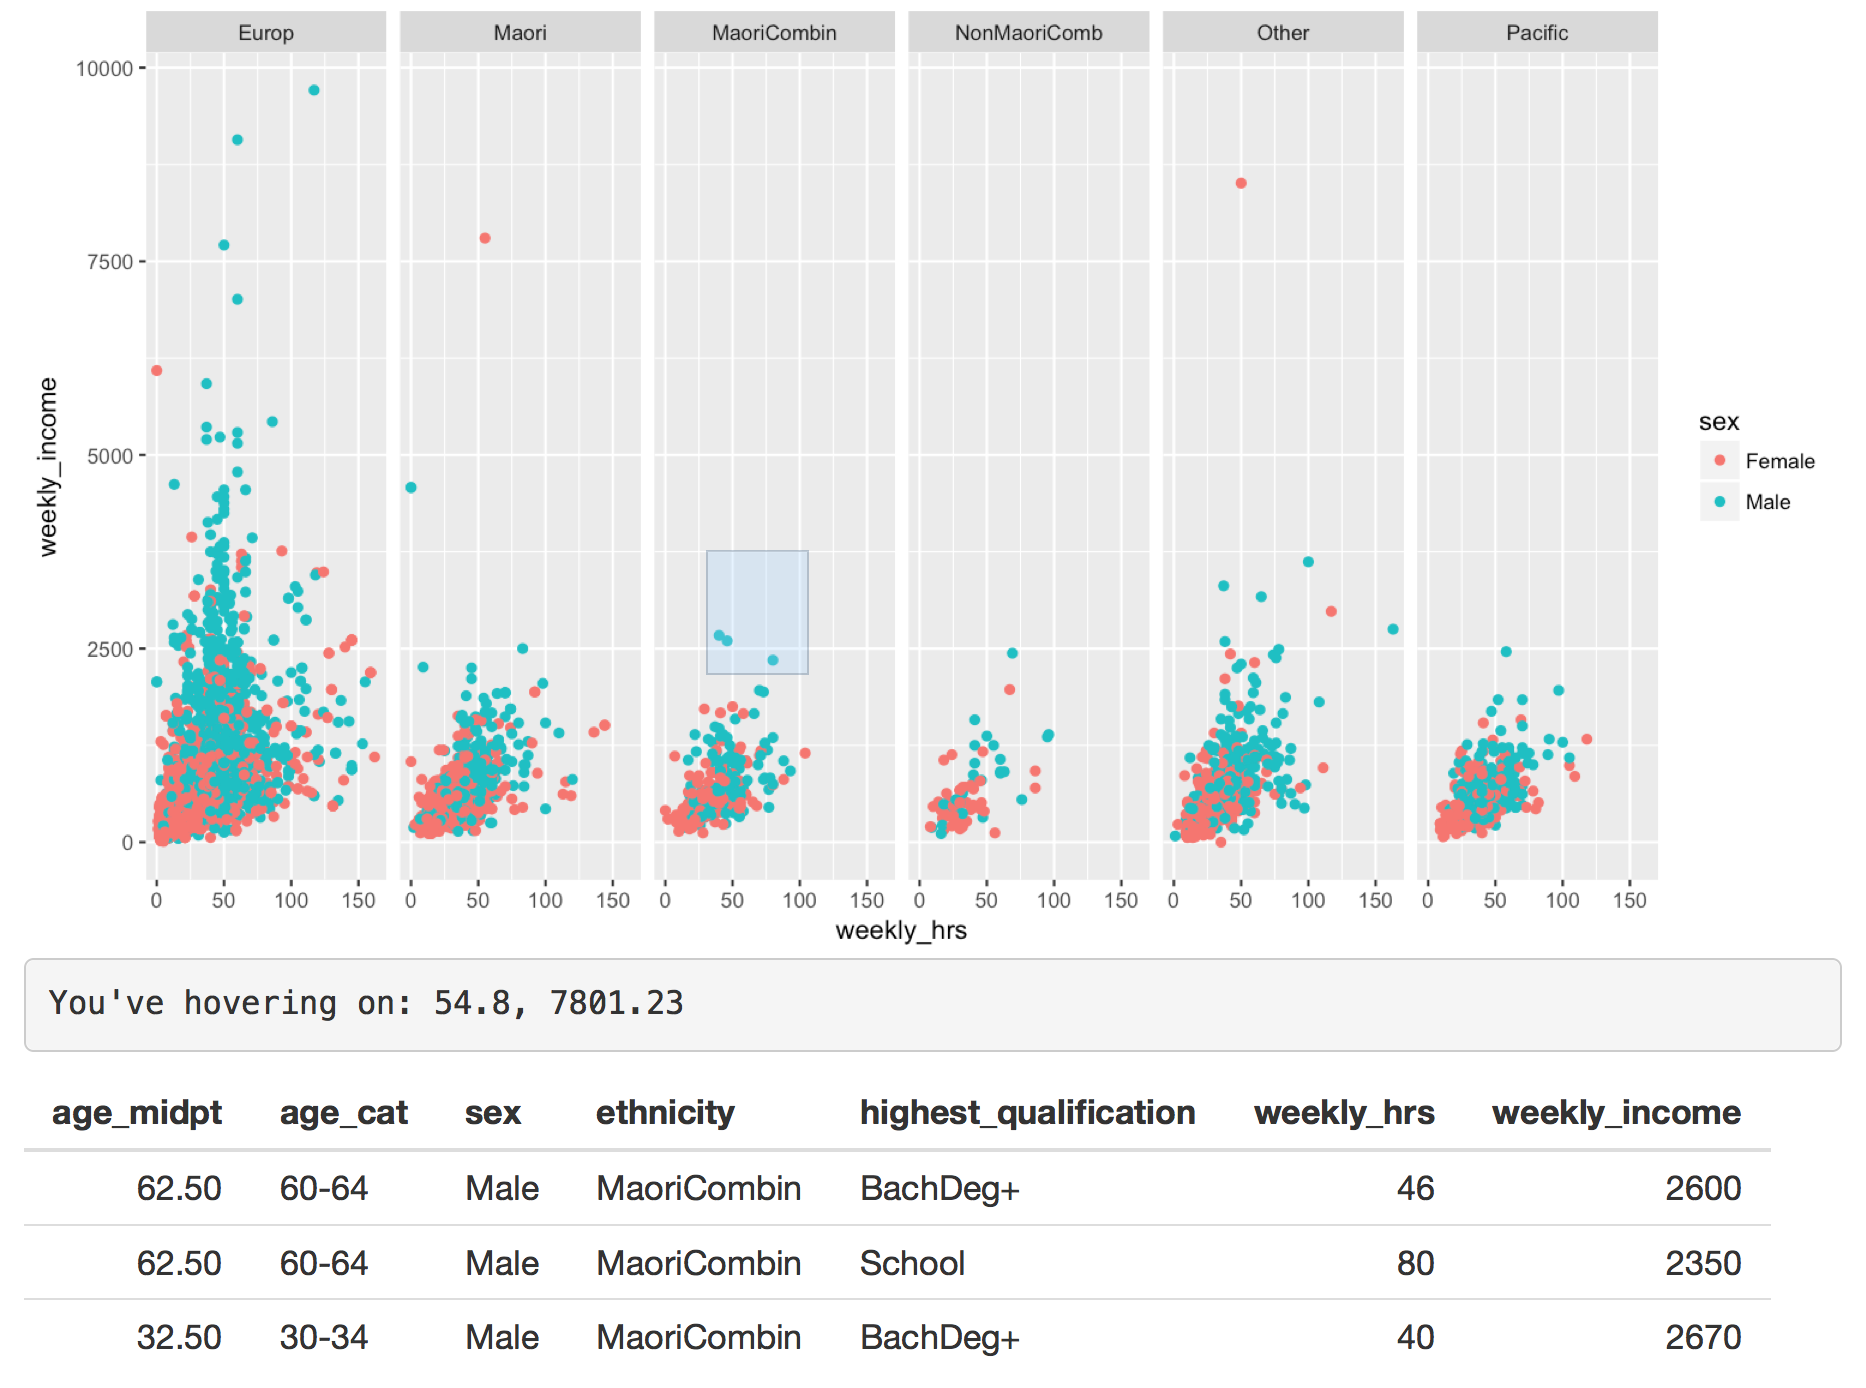
\includegraphics[width=0.6\linewidth,]{./fig/inc-shiny-1} 

}

\caption{\label{fig:inc-shiny-1} Facetted ggplot with linked brushing and hovers}\label{fig:unnamed-chunk-20}
\end{figure}

However, these basic interactive tools only work on base R plots or
plots rendered with \textbf{ggplot2} and best with scatter plots. It is
possible to extend this to bar plots, but it requires more thought. This
is because the pixel co-ordinates of the plot are correctly mapped to
the data (RStudio 2017b). When we try this on a lattice plot as seen
below in \autoref{fig:inc-shiny-2}, this mapping condition fails as the
co-ordinates system differs between the data and the plot itself. It is
possible to create your own mappings to a plot or image, however it is
complex to develop.

\begin{figure}[H]

{\centering 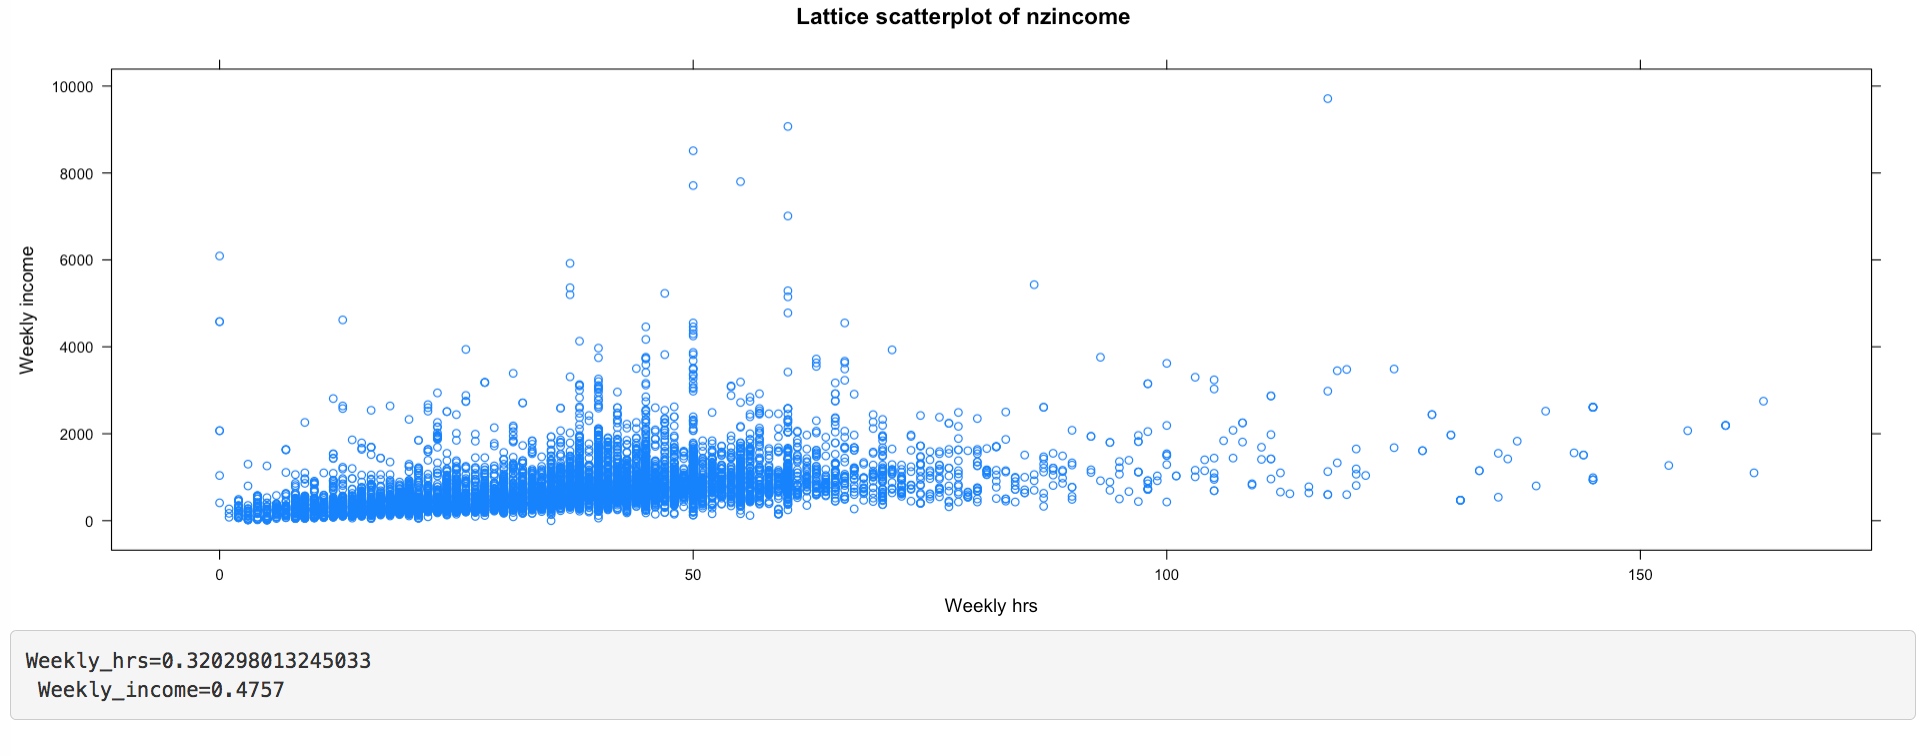
\includegraphics[width=0.6\linewidth,]{./fig/inc-shiny-2} 

}

\caption{\label{fig:inc-shiny-2} A lattice plot that fails to produce correct mapping}\label{fig:unnamed-chunk-22}
\end{figure}

Because the plots displayed are in an image format, we can only view
these plots as a single object and cannot pull apart elements on the
plot. We are unable to further extend and add onto a plot, such as add a
trend line when brushing or change colours of points when clicked on.
Despite being limited to plot interactions (clicks, brushes and hovers),
we can use \textsf{shiny} to link multiple views of the data set.

\subsection{Linking plotly or ggvis with
shiny}\label{linking-plotly-or-ggvis-with-shiny}

Although \textsf{shiny} is great at facilitating interactions from
outside of a plot, it is limited in facilitating interactions within a
plot. It does not have all the capabilities that \textsf{plotly}
provides. When we combine the two together, more interaction can be
achieved with less effort.

\begin{figure}[H]

{\centering 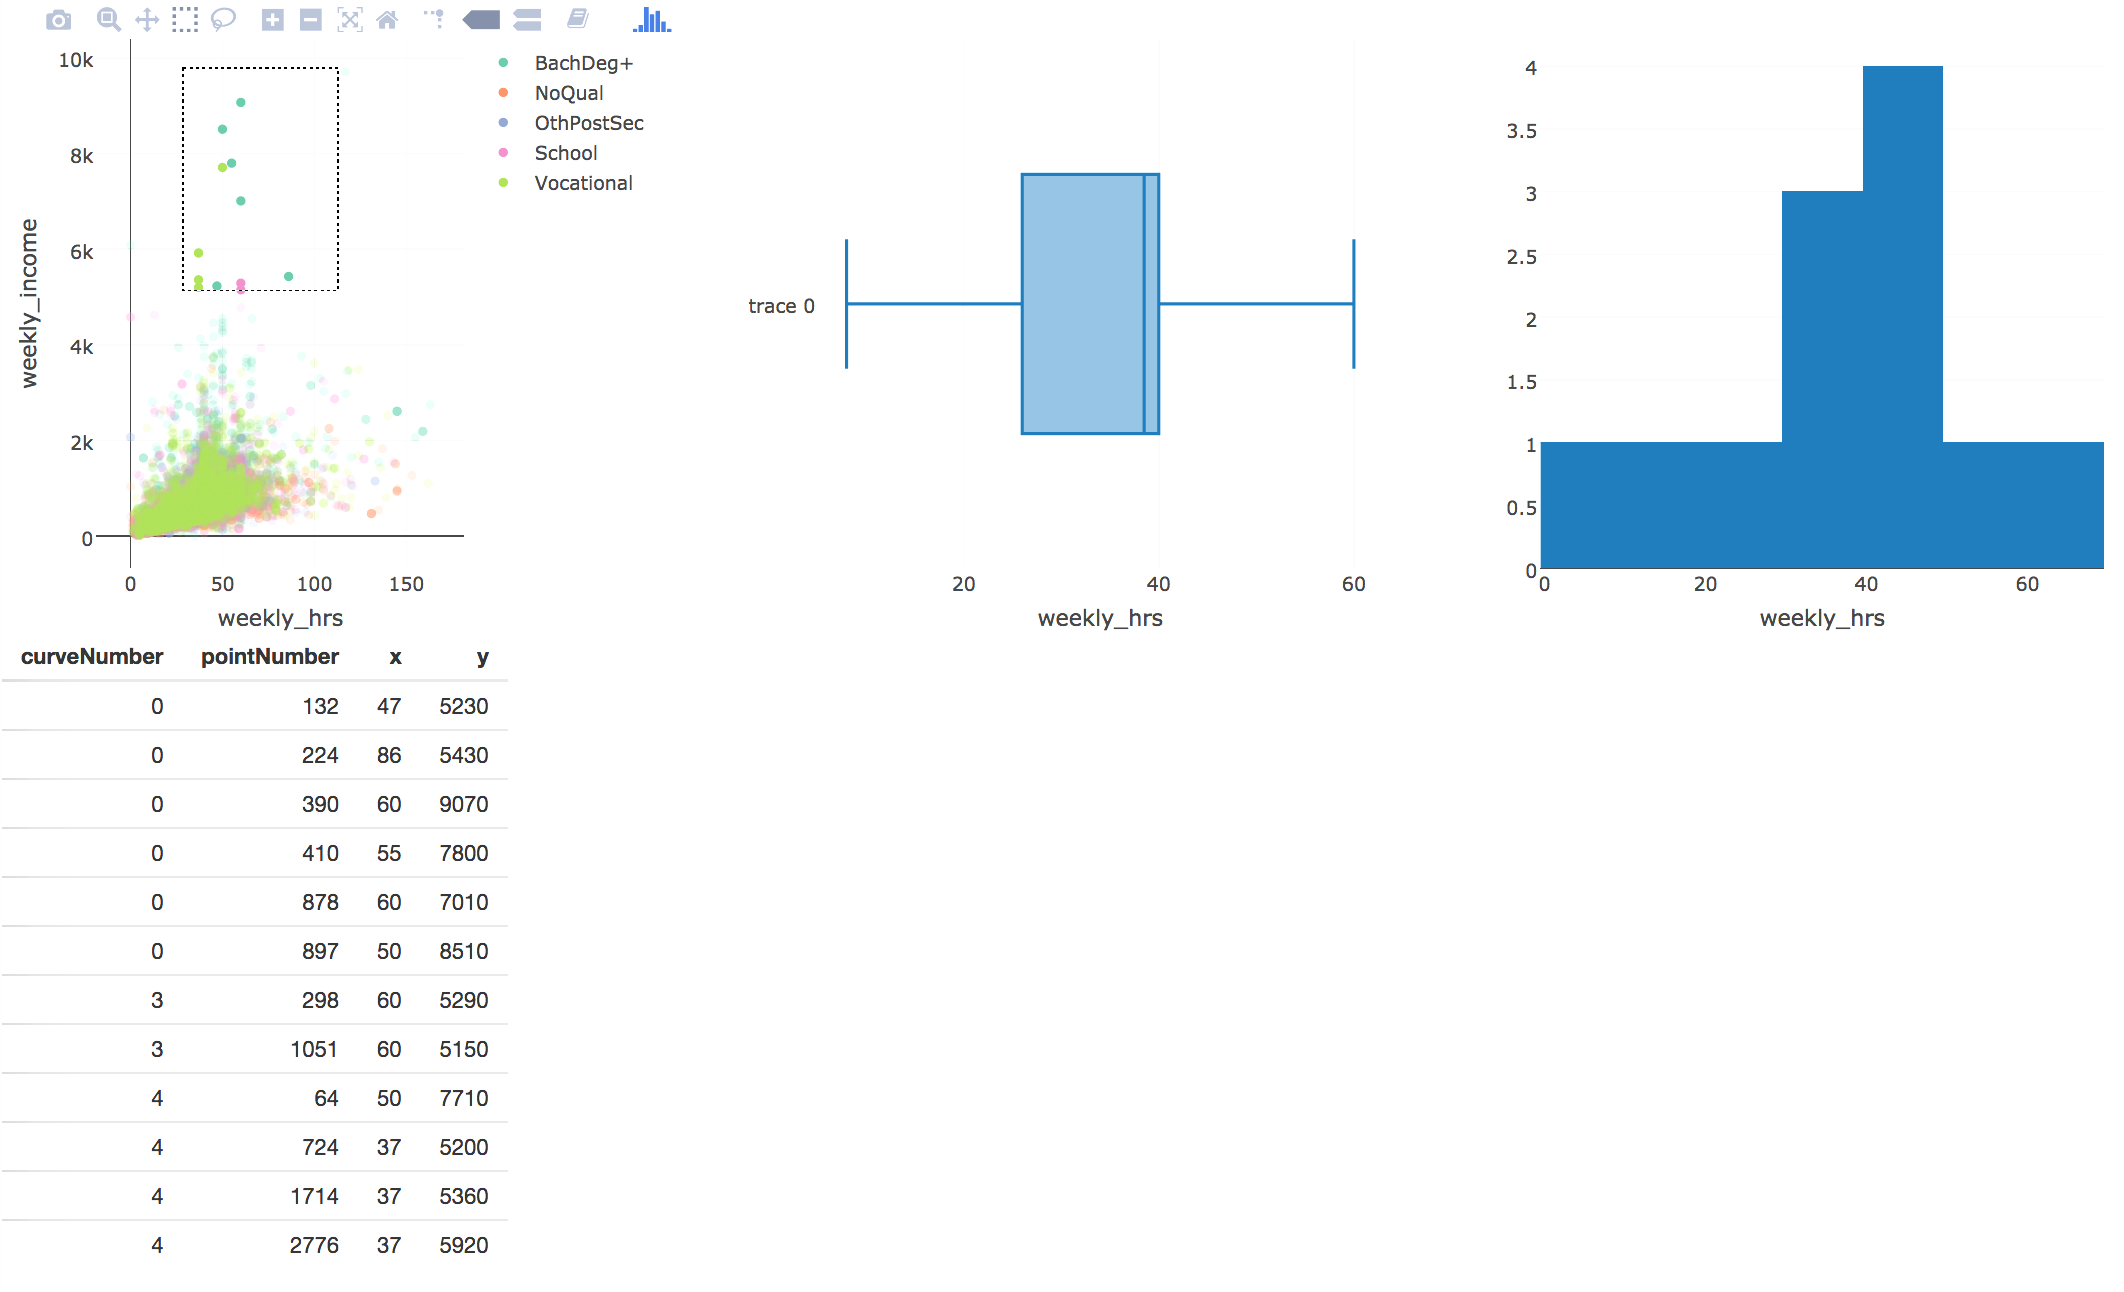
\includegraphics[width=0.7\linewidth,]{./fig/inc-plotly-shiny} 

}

\caption{\label{fig:inc-plotly-shiny} a shiny app with a plotly plot with linked brushing}\label{fig:unnamed-chunk-24}
\end{figure}

\textsf{plotly} (along with many other R packages that generate
htmlwidgets) and ggvis have their own way of incorporating plots into a
shiny application. In \autoref{fig:inc-plotly-shiny}, we can easily
embed plots into \textsf{shiny} using the \texttt{plotlyOutput()}
function. The \textsf{plotly} package also has its own way of
co-ordinating linked brushing and in-plot interactions to other shiny
outputs under a function called \texttt{event\_data()} (Sievert 2017b).
By combining it with \textsf{shiny}, we are able to link different plots
together and to the data itself that is displayed as a table below.
These in-plot interactions are very similar to what \textsf{shiny}
provides for \textbf{graphics} plots and \textbf{ggplot2}. They work
well on scatter plots, but not on other kinds of plots that plotly can
provide. These can help generate or change different outputs on the
page, but not within themselves. By combining the two together, we get
on-plot functionalities from the htmlwidget, with off-plot driven
interactions from shiny. Similarly, when we can combine \textsf{ggvis}
and \textsf{shiny} together we get similar results as seen in
\autoref{fig:inc-ggvis-shiny}. ggvis has its own functions
(\texttt{ggvisOutput()} and \texttt{linked\_brush()}) that allow for
similar interactions to be achieved (Wickham and Chang 2016).

\begin{figure}[H]

{\centering 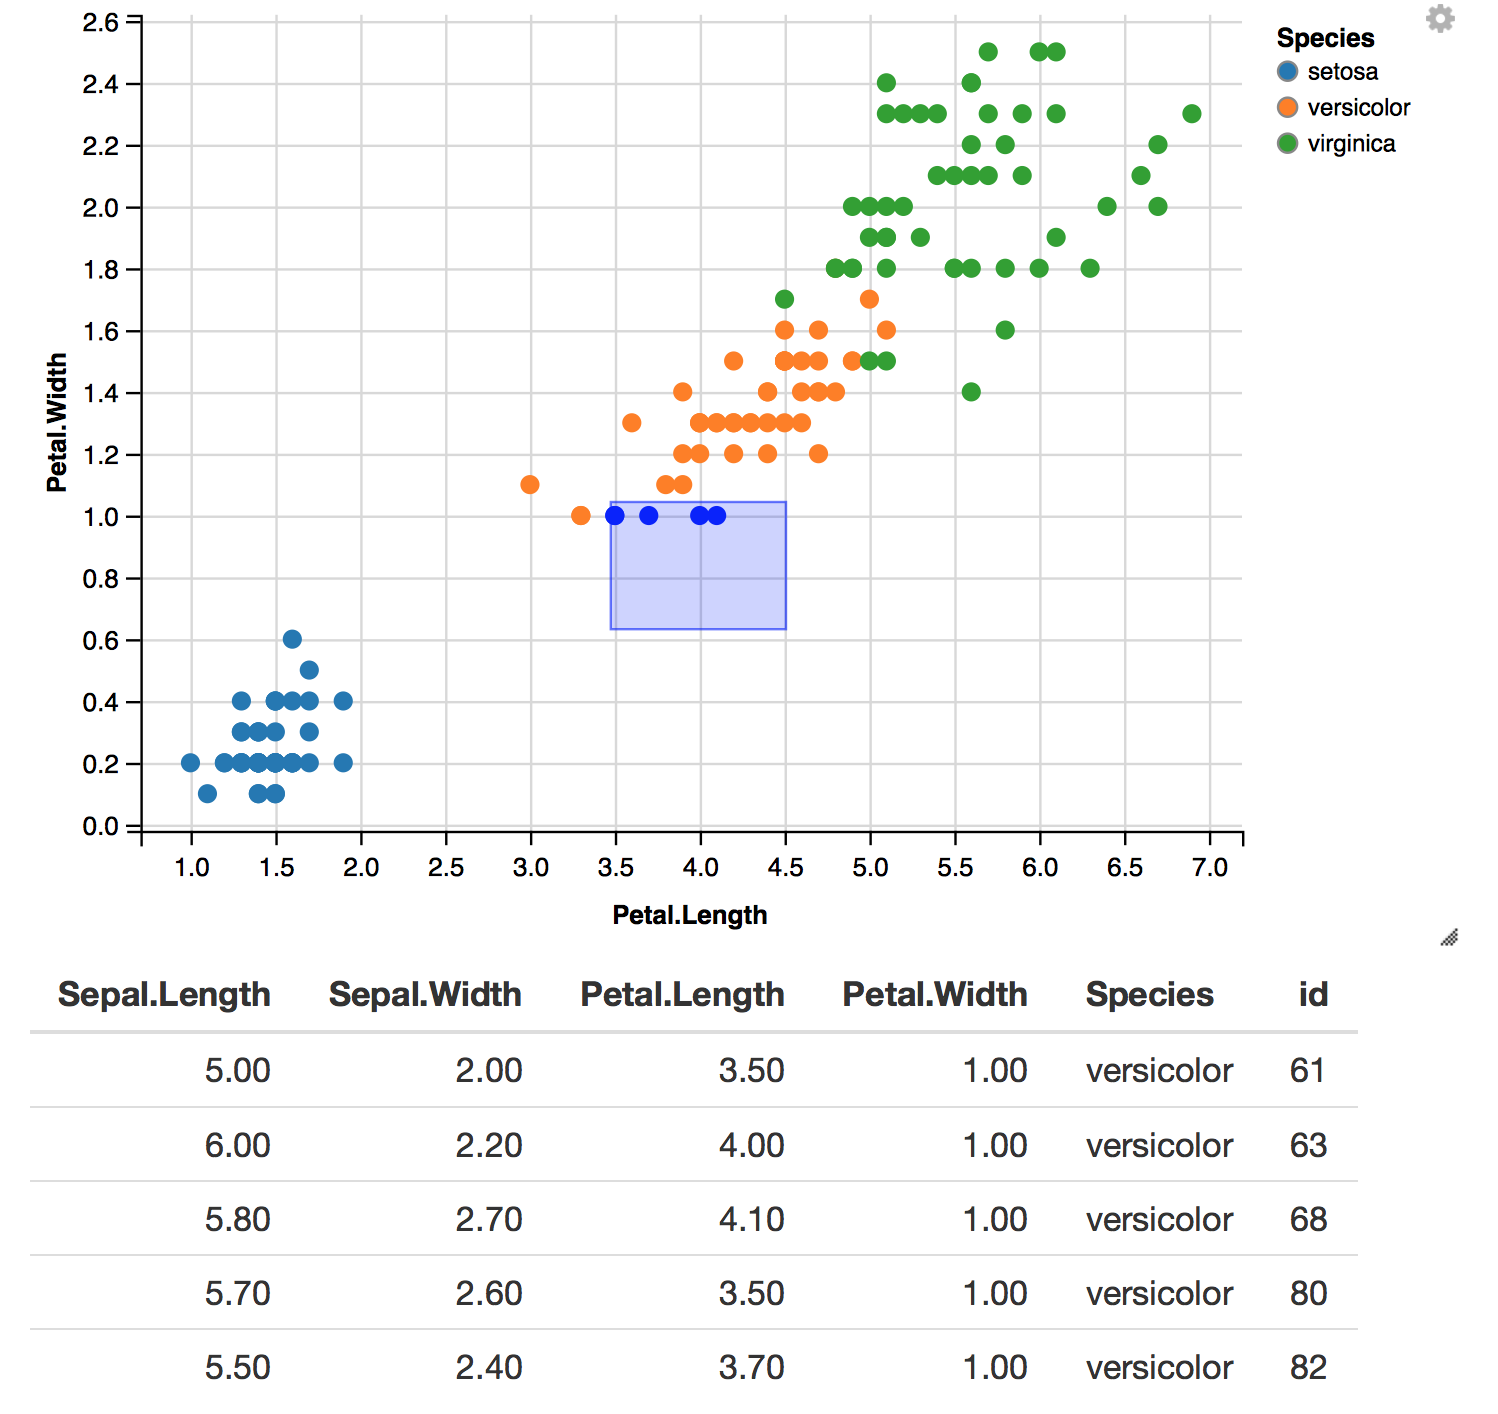
\includegraphics[width=0.7\linewidth,]{./fig/inc-ggvis-shiny} 

}

\caption{\label{fig:inc-ggvis-shiny} an example of linked brushing between ggvis plots}\label{fig:unnamed-chunk-26}
\end{figure}

However, we are still left with a general problem of \textsf{shiny}
(with the exception of \textsf{ggvis}) recomputing and redrawing a plot
or widget every time an input changes. As of writing, work has been
developed to prevent plots generated by plotly to only change certain
parts of a plot whenever a plot is implemented with shiny. As of
writing, this was not possible. However, in a recent version of
plotly(4.7.1), Sievert(2017a) has shown that this is possible with a new
feature called \texttt{plotlyProxy()}, but requires knowledge of the
\texttt{plotly.js} library and how these proxy objects work.

\section{animint}\label{animint}

\textbf{animint} (Hocking et al. 2017) is an R package designed to allow
users to create interactive and animative visuals using
\textbf{ggplot2}. It uses the concept of direct manipulation defined in
Scheiderman (1982). It focuses on adding two main aesthetics to ggplot2
- \texttt{clickSelects} to allow the user to click on a selection, and
\texttt{showSelects} that shows the current selection. The user is able
to directly click on the plot, which can be used to link multiple views
of data on the same page. It uses D3 to generate the interactive plot on
the page, and stores all the data in multiple TSV files that can be
viewed locally.

To illustrate, we create a simple example linking between the groups of
ethnicity to different views of the nzincome data set.

\begin{Shaded}
\begin{Highlighting}[]
\KeywordTok{library}\NormalTok{(animint)}
\NormalTok{plot1 <-}\StringTok{ }\KeywordTok{ggplot}\NormalTok{(income) }\OperatorTok{+}\StringTok{ }\KeywordTok{aes}\NormalTok{(}\DataTypeTok{x =}\NormalTok{ sex, }\DataTypeTok{clickSelects =}\NormalTok{ sex) }\OperatorTok{+}\StringTok{ }\KeywordTok{geom_bar}\NormalTok{()}
\NormalTok{plot2 <-}\StringTok{ }\KeywordTok{ggplot}\NormalTok{(income) }\OperatorTok{+}\StringTok{ }\KeywordTok{aes}\NormalTok{(}\DataTypeTok{x =}\NormalTok{ weekly_hrs, }\DataTypeTok{y =}\NormalTok{ weekly_income, }\DataTypeTok{showSelected =}\NormalTok{ sex,}
                              \DataTypeTok{color =}\NormalTok{ highest_qualification) }\OperatorTok{+}\StringTok{ }\KeywordTok{geom_point}\NormalTok{()}

\NormalTok{plotAll <-}\StringTok{ }\NormalTok{(}\KeywordTok{list}\NormalTok{(}\DataTypeTok{p1 =}\NormalTok{ plot1, }\DataTypeTok{p2 =}\NormalTok{ plot2))}
\KeywordTok{structure}\NormalTok{(plotAll, }\DataTypeTok{class =} \StringTok{"animint"}\NormalTok{)}
\end{Highlighting}
\end{Shaded}

Figure 2.12: animint example

If we click on any of the bars on the bar plot (left), the scatter plot
(right) shows the selected points that correspond that that group.

Hocking's(2017) example of the displaying different views of the World
Bank dataset shows how complex these interactive and animative plots can
be achieved with less than 100 lines of code. It is simple and
straightforward, and is not restricted to linking scatter plots as
discussed with crosstalk and plotly. Because the plots are rendered
entirely in JavaScript using D3, the plots are relatively more
responsive and faster than compared to using a web-server framework like
shiny (which has an overhead cost from communicating between a remote
server with R and the browser).

The key strength of \textbf{animint} is also its weakness as the only
type of interactivity that can be achieved is clicking and showing what
has been selected (Hocking et al. 2017). Currently, it cannot achieve
brushing or zooming. It is only compatible with \textbf{ggplot2}. For
more developed users of \textbf{ggplot2}, not all \texttt{geoms} are
supported, and may remain static when rendered with \textbf{animint}.
Furthermore, because everything is computed and rendered beforehand,
this means that if a selection requires a recomputation in R before it
can be displayed, this is not possible. Hocking (2017) suggests that a
solution to this is to use \textbf{animint} with shiny, but this means
that a new \textbf{animint} plot is rendered every time the user
interacts with it. The unfortunate situation with creating stand-alone
interactive plots this way is that the amount of data that needs to be
generated to power the plots increases as we increase the number of
subsets. If a data set has multiple subsets that need to be rendered,
\textbf{animint} will need to make all the different combinations for
each subset to link every plot together. The more number of subsets and
the larger the dataset, the number of files that need to be generated to
drive the interactive or animated plot increases. In this case, using a
client-server framework like shiny would be more suitable.

The \textbf{animint} package proves itself as a success in implementing
a complex system that achieves simple interactive and animative plots
that can easily linked and implemented by users using clicks and
selection.

\section{Summary}\label{summary}

From assessing all these tools, we can summarise the features and
drawbacks for each tool in the table below.

\begin{longtable}[]{@{}cccccc@{}}
\toprule
\begin{minipage}[b]{0.10\columnwidth}\centering\strut
Tool\strut
\end{minipage} & \begin{minipage}[b]{0.11\columnwidth}\centering\strut
Type of plot\strut
\end{minipage} & \begin{minipage}[b]{0.18\columnwidth}\centering\strut
Compatible with shiny\strut
\end{minipage} & \begin{minipage}[b]{0.18\columnwidth}\centering\strut
Types of interactions\strut
\end{minipage} & \begin{minipage}[b]{0.17\columnwidth}\centering\strut
Redraws entire plot\strut
\end{minipage} & \begin{minipage}[b]{0.09\columnwidth}\centering\strut
Framework type\strut
\end{minipage}\tabularnewline
\midrule
\endhead
\begin{minipage}[t]{0.10\columnwidth}\centering\strut
plotly\strut
\end{minipage} & \begin{minipage}[t]{0.11\columnwidth}\centering\strut
plotly(plotly.js), ggplot2\strut
\end{minipage} & \begin{minipage}[t]{0.18\columnwidth}\centering\strut
Yes\strut
\end{minipage} & \begin{minipage}[t]{0.18\columnwidth}\centering\strut
Clicks, brushing, subsetting, filters\strut
\end{minipage} & \begin{minipage}[t]{0.17\columnwidth}\centering\strut
Yes * (unless proxy)\strut
\end{minipage} & \begin{minipage}[t]{0.09\columnwidth}\centering\strut
standalone HTML\strut
\end{minipage}\tabularnewline
\begin{minipage}[t]{0.10\columnwidth}\centering\strut
ggvis\strut
\end{minipage} & \begin{minipage}[t]{0.11\columnwidth}\centering\strut
ggvis(Vega)\strut
\end{minipage} & \begin{minipage}[t]{0.18\columnwidth}\centering\strut
Yes\strut
\end{minipage} & \begin{minipage}[t]{0.18\columnwidth}\centering\strut
off-plot interactions, hovers, brushing, filters\strut
\end{minipage} & \begin{minipage}[t]{0.17\columnwidth}\centering\strut
No\strut
\end{minipage} & \begin{minipage}[t]{0.09\columnwidth}\centering\strut
client-server\strut
\end{minipage}\tabularnewline
\begin{minipage}[t]{0.10\columnwidth}\centering\strut
shiny\strut
\end{minipage} & \begin{minipage}[t]{0.11\columnwidth}\centering\strut
R plots, anything compatible with it\strut
\end{minipage} & \begin{minipage}[t]{0.18\columnwidth}\centering\strut
-\strut
\end{minipage} & \begin{minipage}[t]{0.18\columnwidth}\centering\strut
clicks, brushing, filters, subsetting, hovers\strut
\end{minipage} & \begin{minipage}[t]{0.17\columnwidth}\centering\strut
Yes\strut
\end{minipage} & \begin{minipage}[t]{0.09\columnwidth}\centering\strut
client-server\strut
\end{minipage}\tabularnewline
\begin{minipage}[t]{0.10\columnwidth}\centering\strut
animint\strut
\end{minipage} & \begin{minipage}[t]{0.11\columnwidth}\centering\strut
ggplot2 (D3)\strut
\end{minipage} & \begin{minipage}[t]{0.18\columnwidth}\centering\strut
Yes\strut
\end{minipage} & \begin{minipage}[t]{0.18\columnwidth}\centering\strut
clicks + selects\strut
\end{minipage} & \begin{minipage}[t]{0.17\columnwidth}\centering\strut
No (unless used with shiny)\strut
\end{minipage} & \begin{minipage}[t]{0.09\columnwidth}\centering\strut
standalone HTML\strut
\end{minipage}\tabularnewline
\bottomrule
\end{longtable}

Table 1: A summary table of all the tools available and their main
capabilities

Note: anything that is compatible with shiny will end up adopting its
client-server framework.

Most of these tools can be extended using shiny. However the general
problem is that when these systems are implemented with shiny (with the
exception of ggvis), every time a user interacts with an input, the plot
or corresponding widgets will be recomputed and redrawn. Furthermore,
many of these do now allow us to customise our own interactions into the
plot. We can use these tools for easily visualise our data with standard
interactive plots, but if the user wishes to customise interactivity or
extend it further, it presents a dead end or a need for learning its
respective API. The other significant factor is that most these tools
use a JavaScript library to render their plots. While graphics plots
generated in R are supported by \textsf{shiny} and ggplot2 across
\textsf{plotly} and \textbf{animint}, there is no support for graphics
generated with other plotting systems in R. Next, we will look at how we
can achieve specific on-plot interactions on static R plots by combining
JavaScript with lower levels tools and avoid reproducing entire plots
whenever the user interacts with it.

\newpage

\chapter{Interactive R plots using lower level
tools}\label{interactive-r-plots-using-lower-level-tools}

Web interactive graphics can be achieved by R users without the
knowledge of HTML, CSS and JavaScript. However, many of these tools use
an external JavaScript library to render their plots. This section
discusses how we can use two lower level packages,
\textsf{gridSVG}(Murrell and Potter 2017) and \textsf{DOM}(Murrell
2016b) to incorporate interactions into R plots and prevent redrawing
entire plots. One approach to avoid this is to target parts of the plot
that need to be updated. We need a system that renders SVG elements but
has a mapping structure that allows elements to be related back to data.
In R, we can use the \textsf{gridSVG} package. By combining
\textsf{gridSVG}, \textsf{shiny} and JavaScript, we are able to update
specific parts of the plot when the user interacts with an input by
passing JavaScript messages between R and the browser. Because
interactions are achieved by manipulating web content using the
\textsf{DOM}, we can alternatively use the \textsf{DOM} package that
directly allows us to drive web content from R without the need for
writing JavaScript. We will discuss how these different approaches work.

\section{gridSVG}\label{gridsvg}

\textsf{gridSVG} (Murrell and Potter 2017) is an R package that allows
for the conversion of grid graphics in R into SVG. This is powerful
because it is easy to attach interactions to specific elements on the
page. The advantage of using \textsf{gridSVG} over others is that there
is a clear mapping structure between elements in the data set and SVG
elements generated. This is not clear in \textsf{plotly} or
\textsf{ggvis} and their JavaScript libraries, which makes it hard to
identify or trace data back to the elements on the page. This also
explains why it may be difficult to customise interactions on the plot.
With \textsf{gridSVG}, we can add JavaScript to \textsf{grid} elements
in R using \texttt{grid.script()} and \texttt{grid.garnish()} (Murrell
and Potter 2014).

\begin{Shaded}
\begin{Highlighting}[]
\KeywordTok{grid.circle}\NormalTok{(}\DataTypeTok{x =} \FloatTok{0.5}\NormalTok{, }\DataTypeTok{y =} \FloatTok{0.5}\NormalTok{, }\DataTypeTok{r =} \FloatTok{0.25}\NormalTok{, }\DataTypeTok{name =} \StringTok{"circle.A"}\NormalTok{,}
            \DataTypeTok{gp =} \KeywordTok{gpar}\NormalTok{(}\DataTypeTok{fill =} \StringTok{"yellow"}\NormalTok{))}

\KeywordTok{grid.garnish}\NormalTok{(}\StringTok{'circle.A'}\NormalTok{, }\DataTypeTok{onmouseover =} \StringTok{"allred()"}\NormalTok{,}
             \DataTypeTok{onmouseout =} \StringTok{"allyellow()"}\NormalTok{, }\StringTok{"pointer-events"}\NormalTok{ =}\StringTok{ "all"}\NormalTok{)}

\KeywordTok{grid.script}\NormalTok{(}\StringTok{"allred = function() \{}
\StringTok{  var circle = document.getElementById('circle.A.1.1');}
\StringTok{  circle.setAttribute('fill', 'red');}
\StringTok{  \}"}\NormalTok{)}

\KeywordTok{grid.script}\NormalTok{(}\StringTok{"allyellow = function() \{}
\StringTok{  var circle = document.getElementById('circle.A.1.1');}
\StringTok{  circle.setAttribute('fill', 'yellow');}
\StringTok{  \}"}\NormalTok{)}

\KeywordTok{grid.export}\NormalTok{(}\StringTok{"circle.svg"}\NormalTok{)}
\end{Highlighting}
\end{Shaded}

\begin{figure}[H]

{\centering 
\includegraphics[width=0.7\linewidth,]{./fig/circle-DOM-1} 

}

\caption{\label{fig:circle-gridSVG} An interactive circle made using gridSVG - when the user hovers over the circle, it will turn red (shown on the right)}\label{fig:unnamed-chunk-30}
\end{figure}

In \autoref{fig:circle-gridSVG}, the circle has been drawn in R, named
and have interactive elements added before being exported out as an SVG.
A simple interaction has been attached to the circle where if the user
hovers over the circle, it will turn red.

This shows that there is a relationship between \textsf{grid} objects
and SVG objects that are generated. In grid, we have named the circle as
\texttt{circle.A}. \textsf{gridSVG} maintains this as an grouped SVG
element with an id attribute of \texttt{circle.A.1}, where inside lies a
single SVG circle element called \texttt{circle.A.1.1}. In R, we can
refer back to these \textsf{grid} objects to attach interactions to
their SVG counterparts.

Another important feature \textsf{gridSVG} has is the ability to
translate between data and SVG coordinates(Murrell and Potter 2012).
Suppose that a plot has been generated. The \texttt{exportCoords}
argument in \texttt{grid.export} is able to generate data that retains
the locations of viewports and scales from the original plot in R
(Murrell and Potter, 2012). We can use this information to convert data
to SVG coordinates and vice versa.

To demonstrate, we have drawn a plot using the \texttt{cars} data set
and exported its coordinate system with its corresponding SVG. We have
separated the svg and the coordinates.

\begin{Shaded}
\begin{Highlighting}[]
\KeywordTok{xyplot}\NormalTok{(dist }\OperatorTok{~}\StringTok{ }\NormalTok{speed, }\DataTypeTok{data =}\NormalTok{ cars)}
\end{Highlighting}
\end{Shaded}

\begin{center}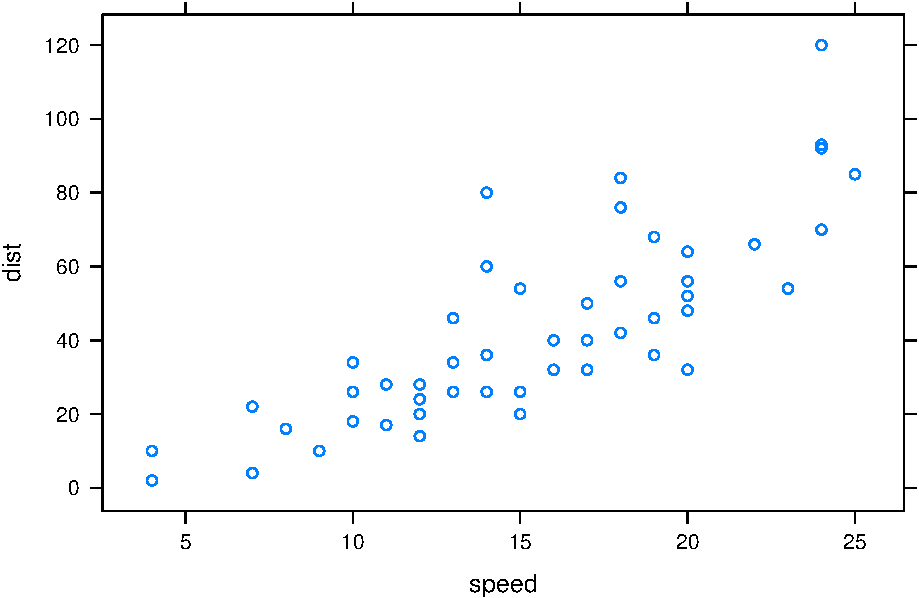
\includegraphics{figures/unnamed-chunk-31-1} \end{center}

\begin{Shaded}
\begin{Highlighting}[]
\NormalTok{svgdoc <-}\StringTok{ }\KeywordTok{grid.export}\NormalTok{(}\OtherTok{NULL}\NormalTok{, }\DataTypeTok{exportCoords =} \StringTok{"inline"}\NormalTok{)}

\CommentTok{# separate the svg and coordinates}
\NormalTok{svg <-}\StringTok{ }\NormalTok{svgdoc}\OperatorTok{$}\NormalTok{svg}
\NormalTok{coords <-}\StringTok{ }\NormalTok{svgdoc}\OperatorTok{$}\NormalTok{coords}
\end{Highlighting}
\end{Shaded}

To be able to use the coordinate system in R to convert between data and
SVG coordinate systems, we need to load it in by calling
\texttt{gridSVGCoords}.

\begin{Shaded}
\begin{Highlighting}[]
\KeywordTok{gridSVGCoords}\NormalTok{(coords)}
\end{Highlighting}
\end{Shaded}

Suppose we have a new point at (4, 5). To be able to convert this in the
correct coordinate space, we need to find the correct viewport
(identified as \texttt{panel}) it lies in. This can then be easily
translated into SVG co-ordinates and back using the functions
\texttt{viewportConvertX} and \texttt{viewportConvertY} with
\texttt{panel}.

\begin{Shaded}
\begin{Highlighting}[]
\CommentTok{# to identify the correct panel:}
\NormalTok{panel <-}\StringTok{ "plot_01.toplevel.vp::plot_01.panel.1.1.vp.2"}

\CommentTok{# if there's a new point we want to find the SVG coordinates of:}
\NormalTok{(x <-}\StringTok{ }\KeywordTok{viewportConvertX}\NormalTok{(panel, }\DecValTok{4}\NormalTok{, }\StringTok{"native"}\NormalTok{))}
\end{Highlighting}
\end{Shaded}

\begin{verbatim}
## [1] 77.92132
\end{verbatim}

\begin{Shaded}
\begin{Highlighting}[]
\NormalTok{(y <-}\StringTok{ }\KeywordTok{viewportConvertY}\NormalTok{(panel, }\DecValTok{5}\NormalTok{, }\StringTok{"native"}\NormalTok{))}
\end{Highlighting}
\end{Shaded}

\begin{verbatim}
## [1] 70.74
\end{verbatim}

The native co-ordinates (4, 5) have been translated as (77.92, 70.74) in
the SVG co-ordinate system. This can be further added on to the web page
without redrawing the rest of the plot as we have the co-ordinates in
the SVG space using JavaScript. We can also translated the coordinates
back into data to return (4, 5).

\begin{Shaded}
\begin{Highlighting}[]
\CommentTok{# to translate back to data (ie native):}
\KeywordTok{viewportConvertX}\NormalTok{(panel, x, }\StringTok{"svg"}\NormalTok{, }\StringTok{"native"}\NormalTok{)}
\end{Highlighting}
\end{Shaded}

\begin{verbatim}
## [1] 4
\end{verbatim}

\begin{Shaded}
\begin{Highlighting}[]
\KeywordTok{viewportConvertY}\NormalTok{(panel, y, }\StringTok{"svg"}\NormalTok{, }\StringTok{"native"}\NormalTok{)}
\end{Highlighting}
\end{Shaded}

\begin{verbatim}
## [1] 5
\end{verbatim}

The main limitations of this package are clear by its name. Only plots
that are defined by the \textsf{grid} graphics system can be converted
into SVG. This means that plots defined using base R cannot be directly
converted (Murrell and Potter 2014). There is a solution to this using
the \textsf{gridGraphics} (Murrell 2015) package that can converts base
R graphics into \textsf{grid} graphics (further demonstrated in Section
4.2.1). Another point to note is that the process of converting elements
to SVG becomes slow when there are many elements to render although work
is under way on this to speed up conversion.

\subsection{Customising simple plot
interactions}\label{customising-simple-plot-interactions}

A clear limitation that is present in the existing tools discussed
previously is letting the user add their own interactions on an existing
plot.

\begin{figure}[H]

{\centering 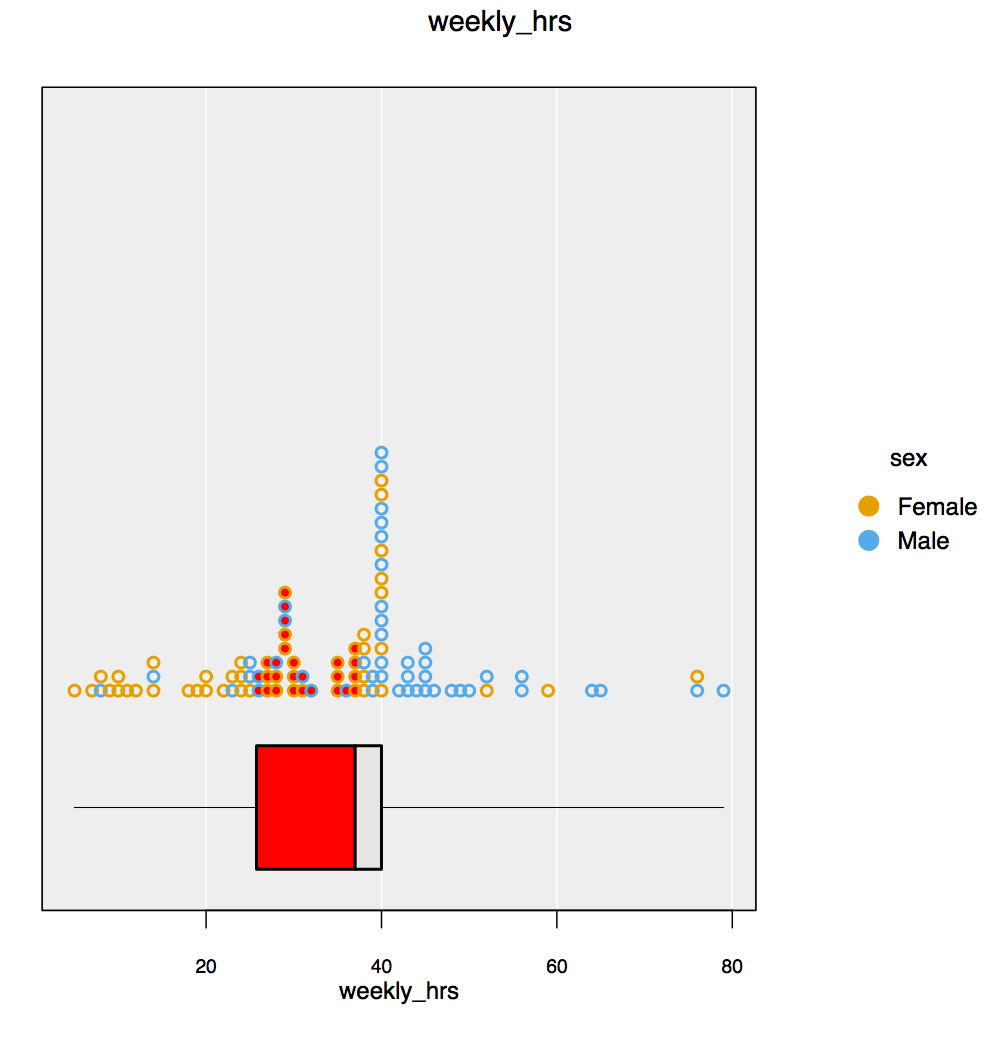
\includegraphics[width=0.7\linewidth,]{./fig/bp-gridSVG} 

}

\caption{\label{fig:bp-gridSVG} An example of a customised box plot interaction on an iNZight plot using gridSVG, JavaScript}\label{fig:unnamed-chunk-35}
\end{figure}

One such example is highlighting part of a box plot to show certain
values between the median and the lower quartile
(\autoref{fig:bp-gridSVG}). When the user clicks on this box, it will
highlight the points that lie within this range. While this can be
achieved with \textsf{gridSVG} and custom JavaScript, it is not as
straightforward with \textsf{plotly} or \textsf{ggvis}. Despite
\textsf{plotly} and \textsf{ggvis} also rendering graphs in SVG, it is
more difficult to identify which elements to target and add interactions
to with these systems.

\subsection{Preventing redraws in shiny using JavaScript messages and
gridSVG}\label{preventing-redraws-in-shiny-using-javascript-messages-and-gridsvg}

As mentioned at the end of Chapter 2, one of the downsides of using
\textsf{shiny} along with \textsf{plotly} or other htmlwidgets is its
nature to redraw plots every time an input changes. With R plots that
are rendered using the \texttt{renderPlot} function, redrawing is
required because the plot is viewed as a raster image. In other cases,
\textsf{shiny} simply re-runs code when a user interacts with an input,
which causes the plot to be redrawn. This means that we cannot
specifically target elements on the page as the plot is viewed as a
single object.

A new approach is to render the plot in SVG and target certain elements
that need to be redrawn while using \textsf{shiny} to communicate back
to R. If we use SVG, we can separate out which components to target and
add interactions without changing the rest of the plot. A complication
to this is that we can no longer use the usual \textsf{shiny} input and
output functions that link everything on the page. \textsf{shiny} also
does not have specific functions to control SVG content. A different way
to do this is to pass data between the browser and back to R using
JavaScript to change certain elements on the web page. \textsf{shiny}
provides a set of functions that allow for messages to be sent through
this channel using two JavaScript functions:
\texttt{shiny.onInputChange()} and
\texttt{shiny.addCustomMessageHandler()} (Heckmann 2013). To send data
from the browser back to R, we use \texttt{shiny.onInputChange()}. This
allows JavaScript objects to be sent back to the \textsf{shiny} server
in a way which can be recognised in R. To send data from R back to the
browser, we use \texttt{shiny.addCustomMessageHandler()}.

To demonstrate how this is useful in updating certain parts of a plot,
we provide an example by altering a smoothing curve using
\textsf{gridSVG} and these JavaScript functions. First, we use
\textsf{gridSVG} to generate our plot and identify the element
corresponding to the trend line. We also need to export the coordinates
in order to be able to transform data into the correct SVG coordinates
when we update the co-ordinates of trend line.

\begin{figure}[H]

{\centering 
\includegraphics[width=1\linewidth,]{./fig/tl-shiny-diagram} 

}

\caption{\label{fig:tl-shiny-diagram} Diagram of how things work using shiny's JavaScript functions in Figure 3.4}\label{fig:unnamed-chunk-36}
\end{figure}

In \autoref{fig:tl-shiny-diagram}, we can pass the degree of smoothing
value from the slider back to R. R then recalculates the x and y
co-ordinates of the new smooth. Once these co-ordinates are calculated,
they are sent back to the browser using
\texttt{session\$sendCustomMessage}. These coordinates are passed to
\texttt{shiny.addCustomMessageHandler()} to run a JavaScript function
that will update the points of the line. This process is used in
\autoref{fig:tl-shiny} with a lattice plot of the iris data set.

\begin{figure}[H]

{\centering 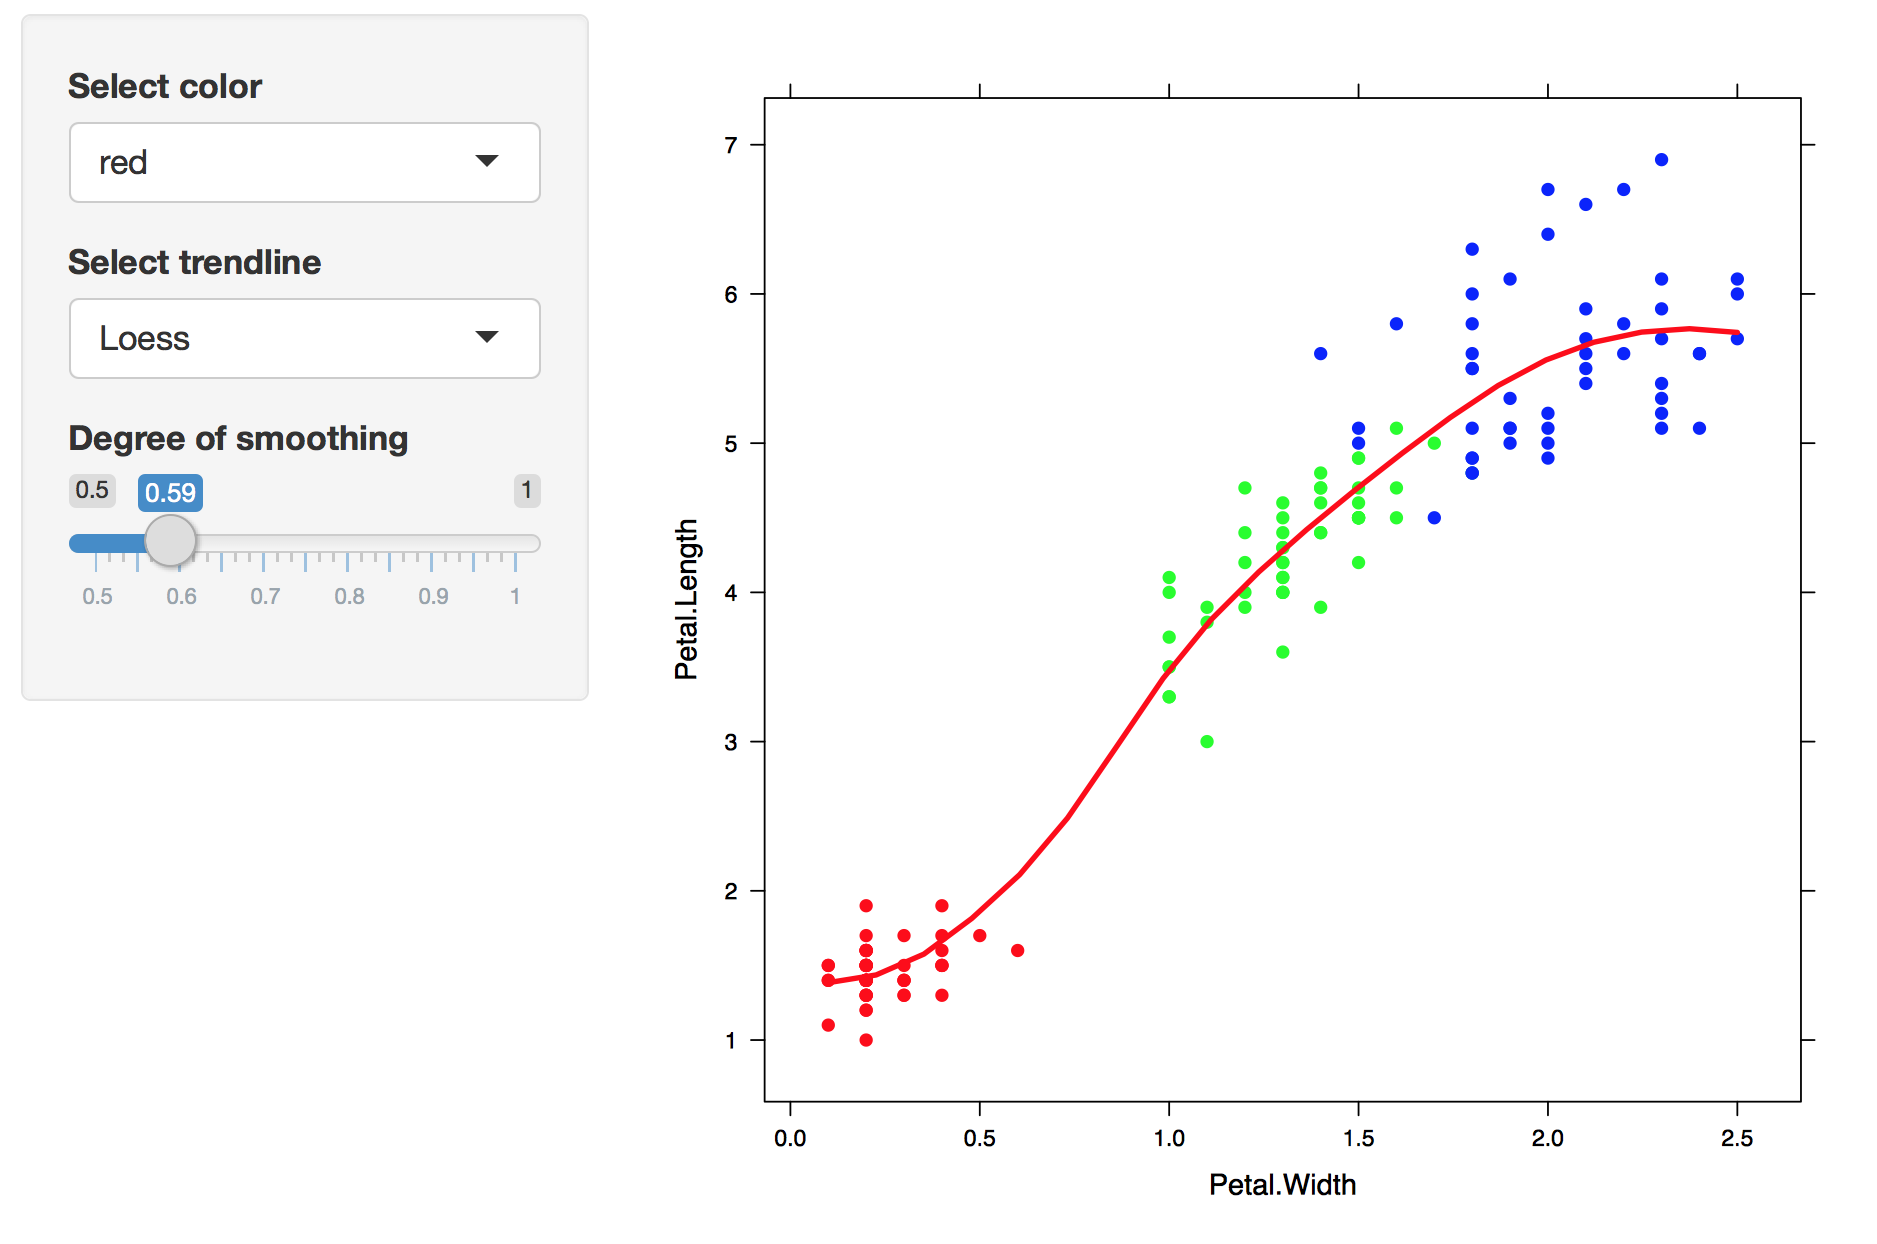
\includegraphics[width=0.7\linewidth,]{./fig/tl-shiny} 

}

\caption{\label{fig:tl-shiny} A replica of Figure 2.7, but only the trendline changes}\label{fig:unnamed-chunk-37}
\end{figure}

This example (\autoref{fig:tl-shiny}) is extensible as we can render
\textsf{grid} graphics (such as \textsf{lattice}) and customise
interactions while maintaining a connection between R and the browser
using \textsf{shiny}. By doing this rather than redrawing the entire
plot, we have only changed the trend line. This method does, however,
require the knowledge of JavaScript and the limitations of how much
information can be sent through are unknown as it is not commonly used.

To stretch this example further, we added in a feature where the user
can highlight over a set of points by dragging the mouse (as seen in
\autoref{fig:tl-shiny-2}). We return the information about these
highlighted points in order to further compute a smoother for just these
points. To achieve this in \textsf{shiny}, we have written some
JavaScript that returns the indices of these selected points back to R
with \texttt{shiny.onInputChange()} to compute a suitable smoother which
is then displayed.

\begin{figure}[H]

{\centering 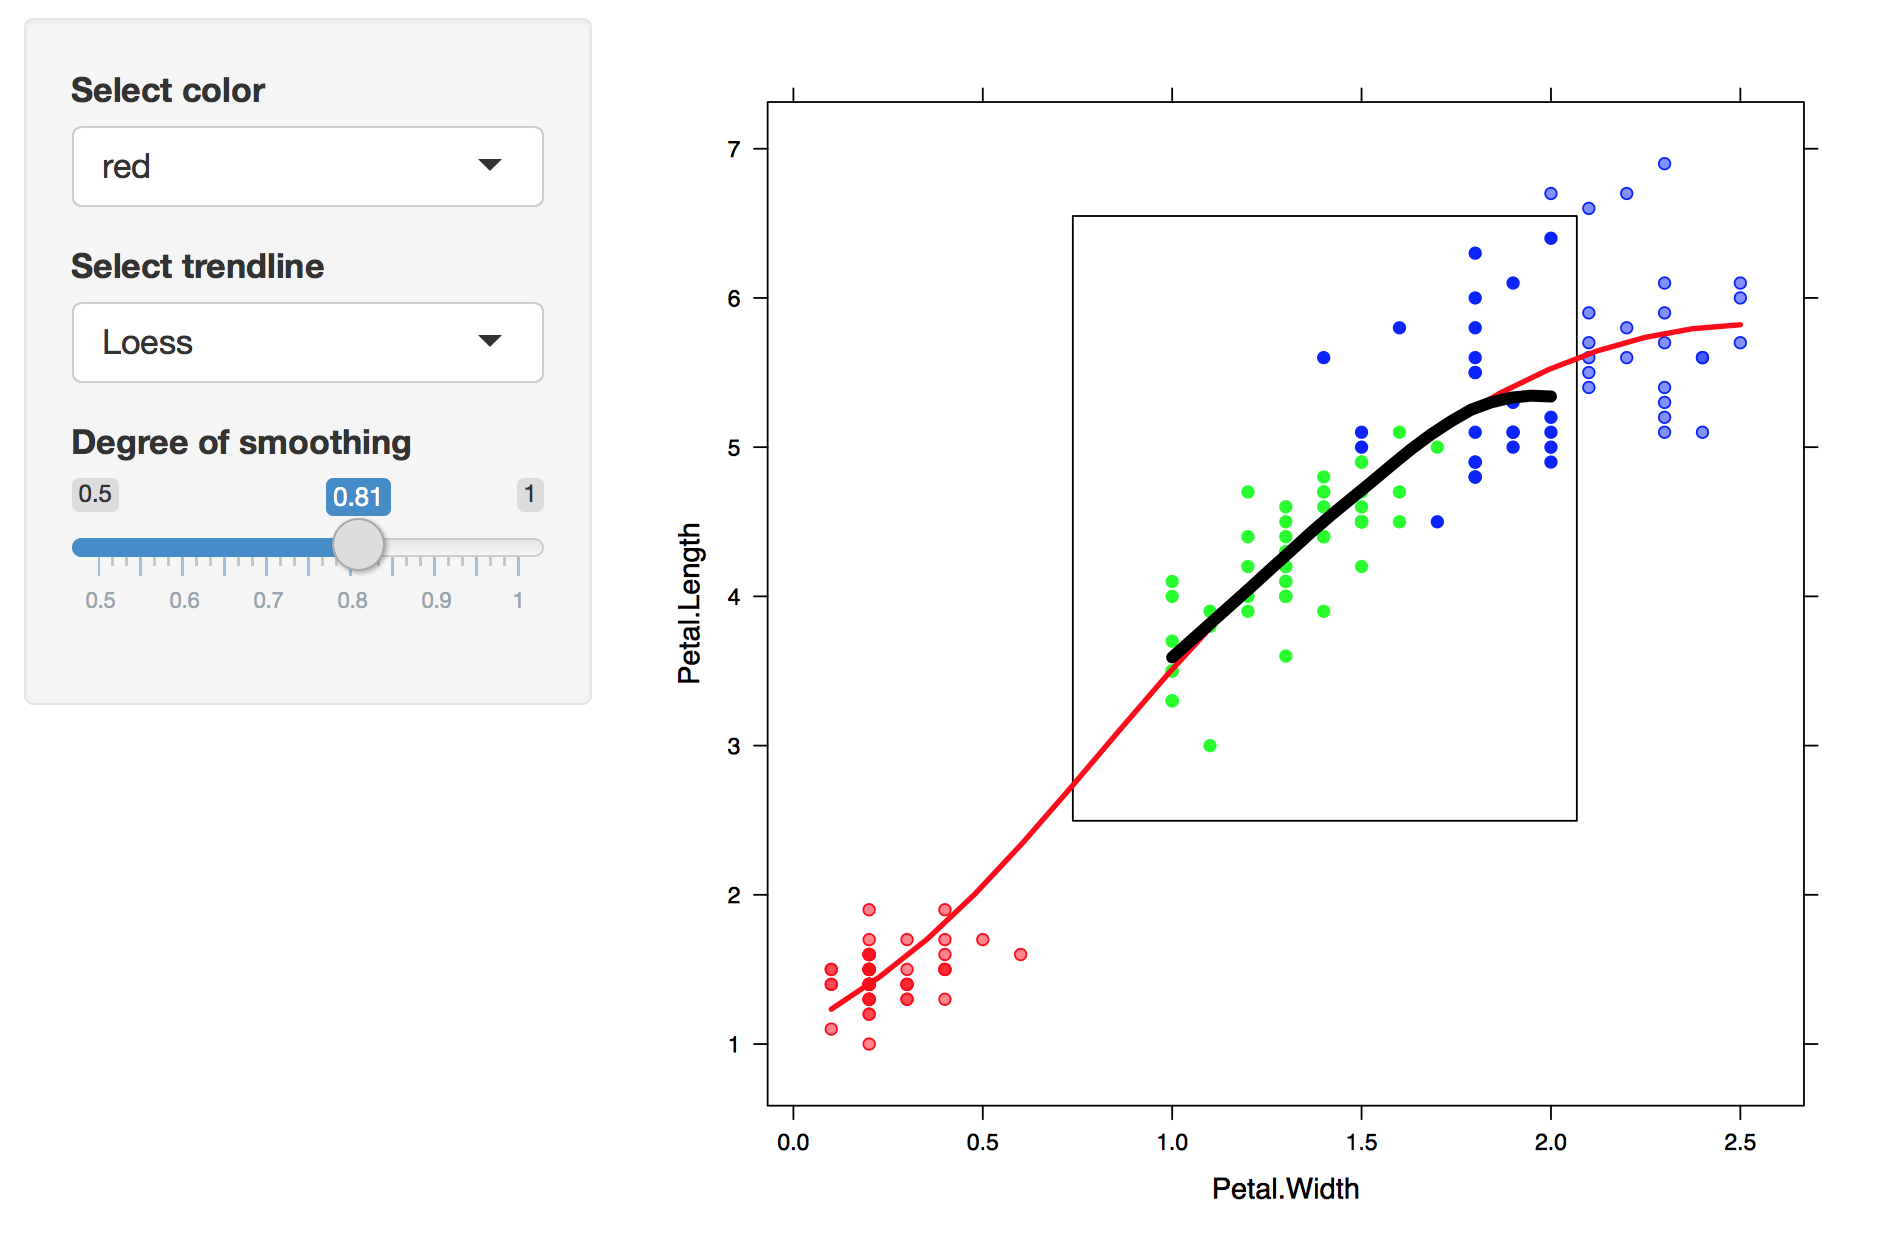
\includegraphics[width=0.7\linewidth,]{./fig/tl-shiny-2} 

}

\caption{\label{fig:tl-shiny-2} Select over a set a points to show a smoother}\label{fig:unnamed-chunk-38}
\end{figure}

\section{DOM package}\label{dom-package}

As highlighted in section 1, many interactions driven on the web are
done by \textsf{DOM} (Document Object Model) manipulation. In brief, the
Document Object Model is a programming interface that allows developers
to manipulate content on a web page (W3C 2009). We can use it to
navigate and pinpoint specific elements on the page to modify and add
interactions to. Generally, this is accessed through by writing
JavaScript functions.

Because most interactions are driven by JavaScript and involve modifying
content on the page, the \textsf{DOM} package (Murrell 2016b) allows for
us to directly do this from R. We can send requests back and forth
between R and the browser. This provides a basis for using the web
browser as an `interactive output device' (Murrell 2016a).

Using the \textsf{DOM} package allows us to write certain commands that
are analogous to what is written in JavaScript. This removes the burden
of traversing between the two programming languages. Rather than writing
JavaScript, we can write \textsf{DOM} commands in R that produce similar
results. Going back to our circle example in Figure 3.1, we can change
the colour of the circle by directly sending this request to the web
page.

\begin{Shaded}
\begin{Highlighting}[]
\CommentTok{#changing the circle to red:}
\NormalTok{circle <-}\StringTok{ }\KeywordTok{getElementById}\NormalTok{(page, }\StringTok{"circle.A.1.1"}\NormalTok{, }\DataTypeTok{response =} \KeywordTok{nodePtr}\NormalTok{())}
\KeywordTok{setAttribute}\NormalTok{(page, circle, }\StringTok{"fill"}\NormalTok{, }\StringTok{"red"}\NormalTok{)}
\end{Highlighting}
\end{Shaded}

In contrast, the JavaScript code for changing this circle from yellow to
red:

\begin{Shaded}
\begin{Highlighting}[]
\KeywordTok{var}\NormalTok{ circle }\OperatorTok{=} \VariableTok{document}\NormalTok{.}\AttributeTok{getElementById}\NormalTok{(}\StringTok{'circle.A.1.1'}\NormalTok{)}\OperatorTok{;}
\VariableTok{circle}\NormalTok{.}\AttributeTok{setAttribute}\NormalTok{(fill}\OperatorTok{,} \StringTok{"red"}\NormalTok{)}\OperatorTok{;}
\end{Highlighting}
\end{Shaded}

The \textsf{DOM} package is also special in which we are able to do
asynchronous programming (\texttt{async\ =\ TRUE}) (Murrell 2016a).
Asynchronous programming is a concept where we are able to start an
initial task and run different tasks at the same time. Here, the
\textsf{DOM} package is able to run a task from R to the browser but
also be able to run commands in R while the call to the browser is still
running. This is important as it makes our web applications more
efficient than trying to run each command or task one at a time. When we
need to call back to R from the browser, these are all asynchronous
events that can easily react to user interactions, making it more
responsive and creates a smoother experience for the user.

\textsf{DOM} allows R to be called from the browser and for requests
from R to be sent to the browser. To demonstrate this, we will replicate
the hover effects on the circle as shown in Figure 3.1.
\autoref{fig:circle-DOM-diagram} shows how this can be set up using
\textsf{DOM}. We can use \texttt{setAttribute} to set the colour of the
circle, and use the \texttt{RDOM.Rcall} function to send requests from
the browser back to R. When the user hovers over the circle, the browser
will send a request back to R to run the \texttt{turnRed} function,
which in turn sends a request back to the browser to change the colour
of the circle to red. Once the user hovers out, the browser will send a
request back to R to turn it back to yellow. Our result is shown in
\autoref{fig:circle-DOM-1}.

\begin{figure}[H]

{\centering 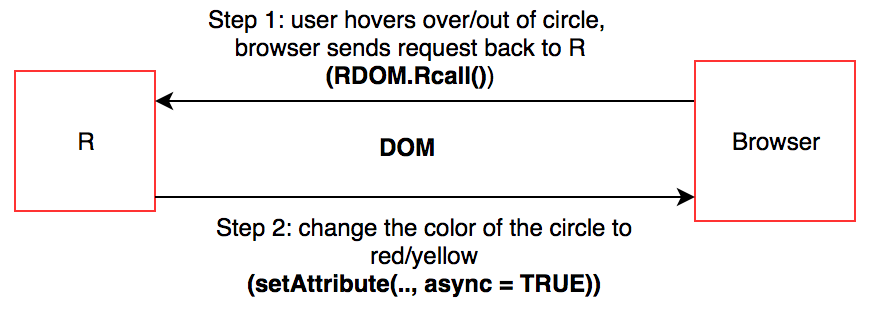
\includegraphics[width=0.7\linewidth,]{./fig/circle-DOM-diagram} 

}

\caption{\label{fig:circle-DOM-diagram} Simple diagram showing how DOM works with from replicating Figure 3.1}\label{fig:unnamed-chunk-41}
\end{figure}

\begin{figure}[H]

{\centering 
\includegraphics[width=0.7\linewidth,]{./fig/circle-DOM-1} 

}

\caption{\label{fig:circle-DOM-1} DOM example of Figure 3.1 - when hovered, the circle turns red (right)}\label{fig:unnamed-chunk-42}
\end{figure}

\begin{Shaded}
\begin{Highlighting}[]
\CommentTok{#draw circle in grid}
\NormalTok{grid}\OperatorTok{::}\KeywordTok{grid.circle}\NormalTok{(}\DataTypeTok{x =} \FloatTok{0.5}\NormalTok{, }\DataTypeTok{y =} \FloatTok{0.5}\NormalTok{, }\DataTypeTok{r =} \FloatTok{0.25}\NormalTok{,}
                  \DataTypeTok{name =} \StringTok{"circle.A"}\NormalTok{, }\DataTypeTok{gp =} \KeywordTok{gpar}\NormalTok{(}\DataTypeTok{fill =} \StringTok{"yellow"}\NormalTok{))}
\CommentTok{#export SVG}
\NormalTok{svg <-}\StringTok{ }\NormalTok{gridSVG}\OperatorTok{::}\KeywordTok{grid.export}\NormalTok{(}\OtherTok{NULL}\NormalTok{)}\OperatorTok{$}\NormalTok{svg}
\KeywordTok{dev.off}\NormalTok{()}

\CommentTok{#set up new page and add circle:}
\KeywordTok{library}\NormalTok{(DOM)}
\NormalTok{page <-}\StringTok{ }\KeywordTok{htmlPage}\NormalTok{()}
\KeywordTok{appendChild}\NormalTok{(page,}
            \DataTypeTok{child =} \KeywordTok{svgNode}\NormalTok{(XML}\OperatorTok{::}\KeywordTok{saveXML}\NormalTok{(svg)),}
            \DataTypeTok{ns =} \OtherTok{TRUE}\NormalTok{,}
            \DataTypeTok{response =} \KeywordTok{svgNode}\NormalTok{())}

\NormalTok{circle <-}\StringTok{ }\KeywordTok{getElementById}\NormalTok{(page, }\StringTok{"circle.A.1.1"}\NormalTok{, }\DataTypeTok{response =} \KeywordTok{nodePtr}\NormalTok{())}
\CommentTok{# hover effects:}
\NormalTok{turnRed <-}\StringTok{ }\ControlFlowTok{function}\NormalTok{(ptr) \{}
  \KeywordTok{setAttribute}\NormalTok{(page,}
\NormalTok{              circle,}
              \StringTok{"fill"}\NormalTok{,}
              \StringTok{"red"}\NormalTok{,}
              \DataTypeTok{async =} \OtherTok{TRUE}\NormalTok{)}
\NormalTok{\}}

\NormalTok{turnYellow <-}\StringTok{ }\ControlFlowTok{function}\NormalTok{(ptr) \{}
  \KeywordTok{setAttribute}\NormalTok{(page,}
\NormalTok{              circle,}
              \StringTok{"fill"}\NormalTok{,}
              \StringTok{"yellow"}\NormalTok{,}
              \DataTypeTok{async =} \OtherTok{TRUE}\NormalTok{)}
\NormalTok{\}}

\KeywordTok{setAttribute}\NormalTok{(page,}
\NormalTok{             circle,}
             \StringTok{"onmouseover"}\NormalTok{,}
             \StringTok{"RDOM.Rcall('turnRed', this, ['ptr'], null)"}\NormalTok{)}

\KeywordTok{setAttribute}\NormalTok{(page,}
\NormalTok{             circle,}
             \StringTok{"onmouseout"}\NormalTok{,}
             \StringTok{"RDOM.Rcall('turnYellow', this, ['ptr'], null)"}\NormalTok{)}
\end{Highlighting}
\end{Shaded}

The example (\autoref{fig:circle-DOM-1}) takes approximately 40 lines of
code for a hover effect. It is much more `lower level' and requires the
user to know how the Document Object Model and main web technologies
work together. A different approach would be to write some JavaScript
and send it across to the browser from R. Since we are only just
changing the colour of the circle, it is more efficient to write
JavaScript and send it to the browser instead rather than telling the
browser to call back to R. It is better to call back to R when a
computation is necessary (such as recomputing a trend line's
co-ordinates in the Section 3.2.1).

\subsection{Comparing DOM to shiny}\label{comparing-dom-to-shiny}

\textsf{DOM} is similar to \textsf{shiny} as it establishes a connection
between R and the browser. To compare, we have replicated
\autoref{fig:tl-shiny} using \textsf{DOM}.

\begin{figure}[H]

{\centering \includegraphics[width=0.7\linewidth,]{./fig/tl-DOM-diagram} 

}

\caption{\label{fig:tl-DOM-diagram} Steps on how a trend line can be altered using the DOM package}\label{fig:unnamed-chunk-44}
\end{figure}

The process of creating this example is similar to what was done with
\textsf{shiny}. However, it is more difficult to set up as it requires
the user to manually link all the components on the page. First, we draw
the plot and save it as an SVG in memory. Next, we can add the SVG plot
and a slider to the page. We identify which element corresponds to the
trend line, and define what happens when the slider moves or when text
is clicked. This requires an additional query to the browser to return
the value of the slider before it can be returned back to R, as shown in
\autoref{fig:tl-DOM-diagram}. These are co-ordinated using asynchronous
callbacks, where once a response is returned, we can schedule another
task behind it. These can be viewed as a series of steps that are linked
together. Once the value of the slider is returned, we can use it to
recalculate the coordinates of the trend line before updating it on the
page. Our final result is put together in \autoref{fig:tl-DOM-2}.

\begin{figure}[H]

{\centering 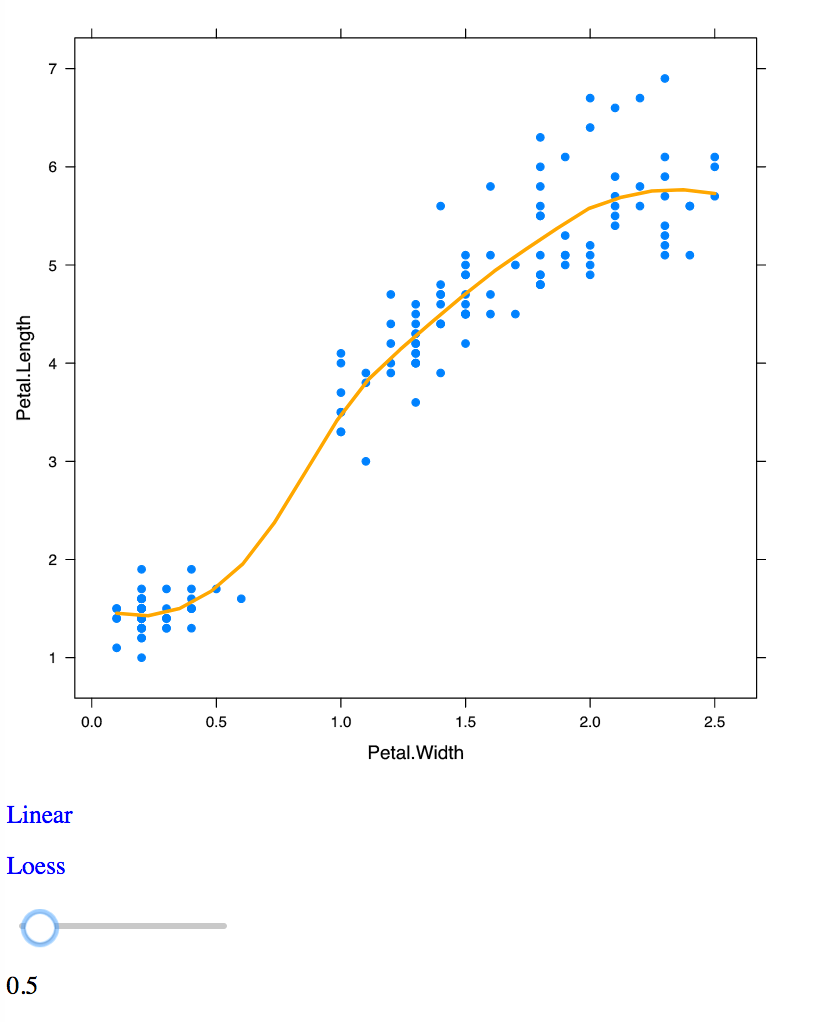
\includegraphics[width=0.5\linewidth,]{./fig/tl-DOM-2} 

}

\caption{\label{fig:tl-DOM-2} DOM example of Fig 3.4 for changing a trend line using a slider}\label{fig:unnamed-chunk-45}
\end{figure}

\textsf{DOM} allows for more flexibility as we have control over the
entire page. From a developer's perspective, we can continue to modify
elements on the page. Users have access to R while the the connection to
the web page is running. We can also run a number of interactive web
pages in a single R session. In \textsf{shiny}, we are unable to use R
in a single session or be able to change it without stopping the
application. Furthermore, a \textsf{shiny} application can only do one
task at a time, and cannot run tasks asynchronously. However, this may
be resolved by the \textsf{promises} package (Cheng 2017b) in the near
future, which allows for asynchronous programming within R and thus,
more responsive \textsf{shiny} applications (Cheng 2017a). A caveat of
using the \textsf{DOM} package is that requires a lot more code to link
everything together. In \textsf{shiny}, these links between inputs and
outputs are much easier to co-ordinate.

Internally, there are many limitations with this package. As this
package is still developmental, only part of the \textsf{DOM} (Document
Object Model) API has been expanded, and the connection between R and
the browser requires extra attention (Murrell 2016a). In some cases, it
is still not possible to achieve certain interactions without
JavaScript, such as capturing where the mouse's position is on screen.
Murrell (2016a) states that it can only be run locally and is currently
aimed at a single user rather than multiple users.

\textsf{gridSVG}, \textsf{DOM} and \textsf{shiny} provide ways in which
we can bind custom JavaScript to elements, but requires the user to be
able to define what kind of interactions they wish to achieve.

There is a clear trade off between existing tools. It is possible to
customise interactions on existing plots, but this requires a knowledge
of JavaScript in order to do so. Comparatively, tools that provide
standard web interactive plots are easier to use but are complex to
modify and extend further. In the next section, we discuss how we can
simplify the implementation of certain interactions on plots originally
rendered in R and build a solution using these tools.

\newpage

\chapter{Designing a more flexible way of producing simple
interactions}\label{designing-a-more-flexible-way-of-producing-simple-interactions}

By using \textsf{gridSVG}, \textsf{DOM} and JavaScript, we can customise
interactions onto plots. However, these are too specific and assume a
lot of knowledge from the user. We need a way to provide interactions
that can be easily customised and defined by the user with a much less
steeper learning curve. This section discusses a potential solution
using grid, \textsf{gridSVG} and \textsf{DOM} to drive web interactive
graphics.

\section{The main idea using grid, gridSVG and
DOM}\label{the-main-idea-using-grid-gridsvg-and-dom}

In each of the previous examples, they is a certain pattern. In order to
define a single interaction, it requires the need to know which SVG
element to target, what type of interaction or event is to be attached
to that element, and how to define what happens when an interaction
occurs. This idea can be broken down into 5 simple steps:

\begin{itemize}
\tightlist
\item
  Draw the plot or elements in R
\item
  Identify elements to interact with
\item
  Determine what kind of interaction is to be achieved
\item
  Attach and link interactions and events to targeted elements
\item
  Send interaction instructions and plot to the browser
\end{itemize}

\begin{figure}[H]
  
  {\centering 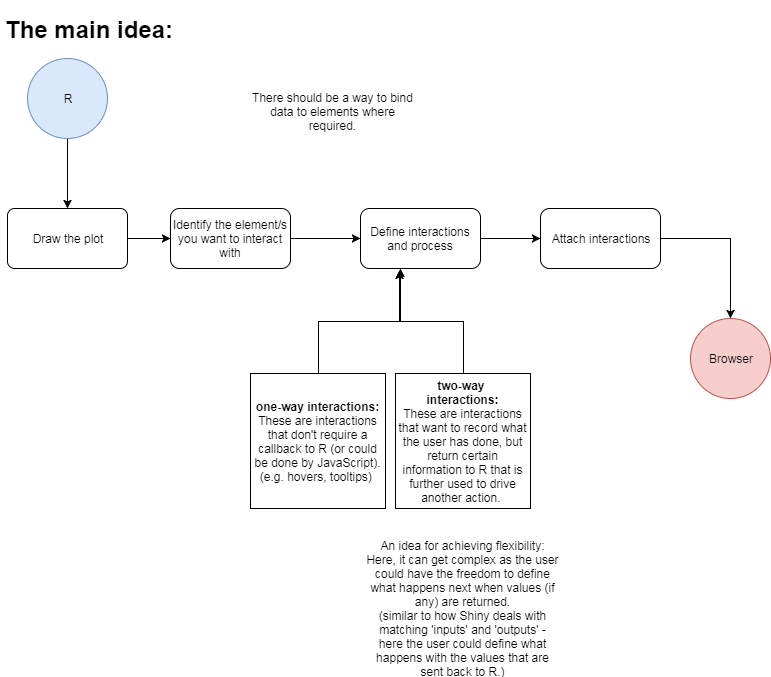
\includegraphics[width=0.7\linewidth,]{./fig/main-idea} 
  
  }
  
  \caption{\label{fig:main-idea} grid, gridSVG and DOM in the process}\label{fig:unnamed-chunk-46}
  \end{figure}

The process above (\autoref{fig:main-idea}) can be implemented using
\textsf{grid}, \textsf{gridSVG} and \textsf{DOM}. We can use the
relationship between \textsf{grid} and \textsf{gridSVG} elements
explained in Section 3.1 to allow users to define and identify which
elements to target. We can use \textsf{DOM} to attach interactions to
certain elements and send these across to a web page. The reason for
using \textsf{DOM} rather than shiny is that there are more complexities
that work under the shiny framework including reactive programming,
which is particularly difficult to grasp in detail. Because it is so low
level, we can use \textsf{DOM} to create different types of
interactions, but it is unreasonable for the majority of users as it
requires some understanding of web technologies and takes too much
effort. As seen in \autoref{fig:circle-DOM-1}, it takes roughly 40 lines
of code to achieve a simple hover effect (with or without writing
JavaScript), and about 200 lines of code to link a slider to a smoother
(\autoref{fig:tl-DOM-2}).

We need a system that is more convenient for users, not too strenuous to
code up, does not require too many pre-requisites, but is flexible
enough to achieve different interactions. We have created the
\textsf{interactr} package that attempts to prototype this idea. It acts
as a convenience wrapper for defining interactions with \textsf{DOM},
\textsf{gridSVG} and \textsf{grid}. It aims to allow users to define
their own interactions to plots in R without the need for a full
understanding of the web technologies involved.

We have recreated some examples using \textsf{interactr} to demonstrate
this idea. Many of the examples discussed below use functions that are
found in this package.

\section{Examples}\label{examples}

\subsection{Linking box plots}\label{linking-box-plots}

The goal for this example is to link the interquartile range of the box
plot to a scatter plot, followed by a density plot. When the user clicks
on the box plot, it highlights the range of the box plot on the other
respective plots.

We note that everything that will be done is coded in R so it requires
no knowledge JavaScript or other web technologies from the user.

Our first step is to draw the box plot in R.

\begin{Shaded}
\begin{Highlighting}[]
\KeywordTok{library}\NormalTok{(interactr)}
\KeywordTok{library}\NormalTok{(lattice)}
\NormalTok{bw <-}\StringTok{ }\KeywordTok{bwplot}\NormalTok{(iris}\OperatorTok{$}\NormalTok{Sepal.Length, }\DataTypeTok{main =} \StringTok{"Sepal length"}\NormalTok{, }\DataTypeTok{xlab =} \StringTok{"Sepal length"}\NormalTok{)}
\end{Highlighting}
\end{Shaded}

Here, we have stored the box plot into a variable called \texttt{bw}. To
attach interactions, we need to identify what elements have been drawn.
We can do that by listing the elements.

\begin{Shaded}
\begin{Highlighting}[]
\KeywordTok{listElements}\NormalTok{(bw)}
\end{Highlighting}
\end{Shaded}

\begin{figure}[H]

{\centering 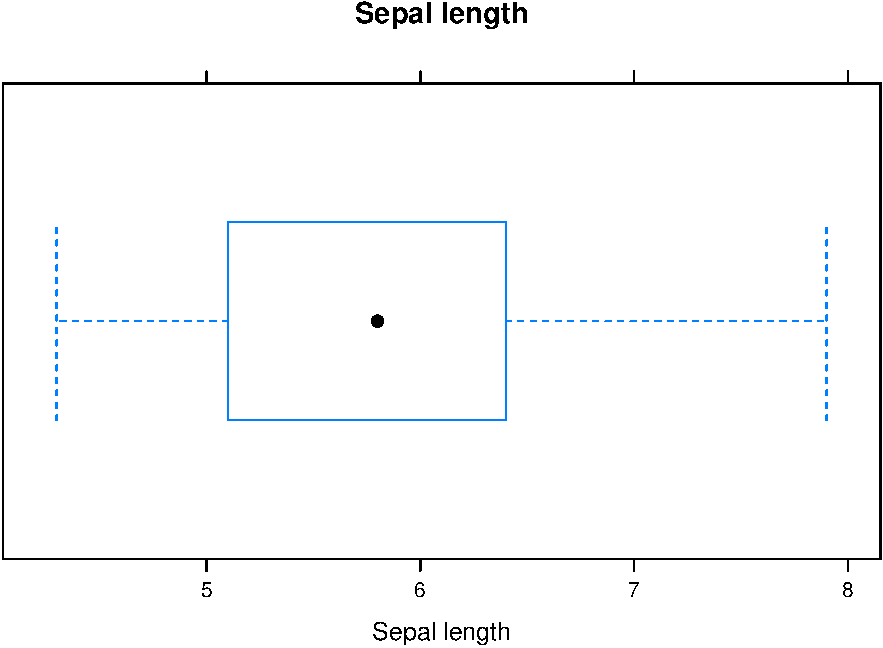
\includegraphics{figures/unnamed-chunk-48-1} 

}

\caption{\label{fig:bp} Producing a box plot in R}\label{fig:unnamed-chunk-48}
\end{figure}

\begin{verbatim}
## plot_01.background
## plot_01.main
## plot_01.xlab
## plot_01.ticks.top.panel.1.1
## plot_01.ticklabels.left.panel.1.1
## plot_01.ticks.bottom.panel.1.1
## plot_01.ticklabels.bottom.panel.1.1
## plot_01.bwplot.box.polygon.panel.1.1
## plot_01.bwplot.whisker.segments.panel.1.1
## plot_01.bwplot.cap.segments.panel.1.1
## plot_01.bwplot.dot.points.panel.1.1
## plot_01.border.panel.1.1
\end{verbatim}

\begin{Shaded}
\begin{Highlighting}[]
\NormalTok{box <-}\StringTok{ "plot_01.bwplot.box.polygon.panel.1.1"}
\end{Highlighting}
\end{Shaded}

This will print the plot (\autoref{fig:bp}) and return a list of all the
elements that make up the box plot in R. The user can identify which
element to target to attach interactions. This is one of the
disadvantages (further discussed in Section 5.2) of this process - the
user must deduce which element to target through the names listed. In
some cases, this is straightforward like in the example above, we
suggest that the `box' should refer to the box plot. We have identified
the box that marks between the lower quartile and upper quartile.

Next, we can define a simple interaction. We want to achieve an
interaction where when the user hovers over the box, it will turn red.
In the case of a hover, we have defined it as a type of interaction to
which we can specify the `attributes' and styles of the box.

\begin{Shaded}
\begin{Highlighting}[]
\NormalTok{interactions <-}\StringTok{ }\KeywordTok{list}\NormalTok{(}\DataTypeTok{hover =} \KeywordTok{styleHover}\NormalTok{(}\DataTypeTok{attrs =} \KeywordTok{list}\NormalTok{(}\DataTypeTok{fill =} \StringTok{"red"}\NormalTok{,}
                                                     \DataTypeTok{fill.opacity =} \StringTok{"1"}\NormalTok{)))}
\end{Highlighting}
\end{Shaded}

Note that the interaction has only been defined but not linked to the
targeted element (which is the box) yet.

\begin{Shaded}
\begin{Highlighting}[]
\KeywordTok{draw}\NormalTok{(bw, box, interactions, }\DataTypeTok{new.page =} \OtherTok{TRUE}\NormalTok{)}
\end{Highlighting}
\end{Shaded}

This line of code (the \texttt{draw} function) both links the
interaction we defined before to the box element and sends the plot
across to a new web page. We see that when the user hovers over the box,
the box turns red as seen in \autoref{fig:int-bp-1}.

\begin{figure}[H]

{\centering 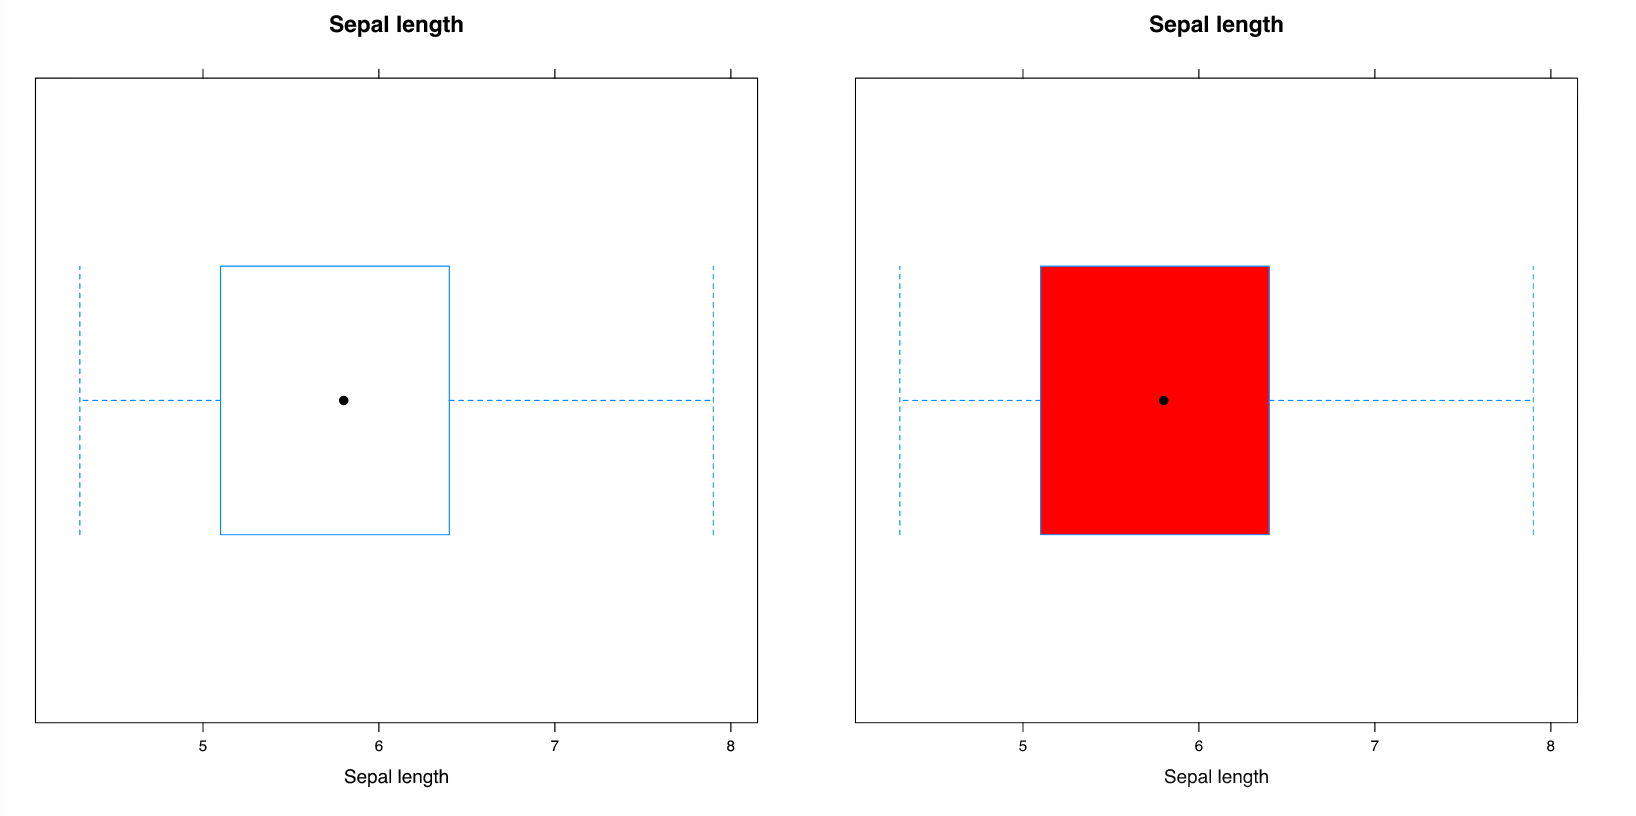
\includegraphics[width=0.7\linewidth,]{./fig/int-bp-1} 

}

\caption{\label{fig:int-bp-1} Box plot with hover interaction}\label{fig:unnamed-chunk-51}
\end{figure}

Before we move on to drawing the scatter plot, we need to make sure we
identify the interquartile range of the box plot and extract any other
information we may require from the plot before moving onto the next.
This is one of the disadvantages of using this package which is further
discussed in Section 5.2 when plots are separately drawn to the graphics
device each time.

Here, we can return the range of the box plot and store it in a variable
called \texttt{range}.

\begin{Shaded}
\begin{Highlighting}[]
\NormalTok{range <-}\StringTok{ }\KeywordTok{returnRange}\NormalTok{(box)}
\end{Highlighting}
\end{Shaded}

We now proceed to add a scatter plot by drawing the scatter plot,
listing the elements and identifying the `points', before sending it to
the same web page.

\begin{Shaded}
\begin{Highlighting}[]
\NormalTok{sp <-}\StringTok{ }\KeywordTok{xyplot}\NormalTok{(Sepal.Width }\OperatorTok{~}\StringTok{ }\NormalTok{Sepal.Length,}
             \DataTypeTok{data =}\NormalTok{ iris,}
             \DataTypeTok{main =} \StringTok{"Sepal Width ~ Sepal Length"}\NormalTok{)}
\KeywordTok{listElements}\NormalTok{(sp)}
\NormalTok{points <-}\StringTok{ "plot_01.xyplot.points.panel.1.1"}
\KeywordTok{draw}\NormalTok{(sp) }\CommentTok{#by default, new.page = FALSE}
\end{Highlighting}
\end{Shaded}

We see that the box plot and the scatter plot we drew in R are now on
the same web page (\autoref{fig:int-bp-2}).

\begin{figure}[H]

{\centering 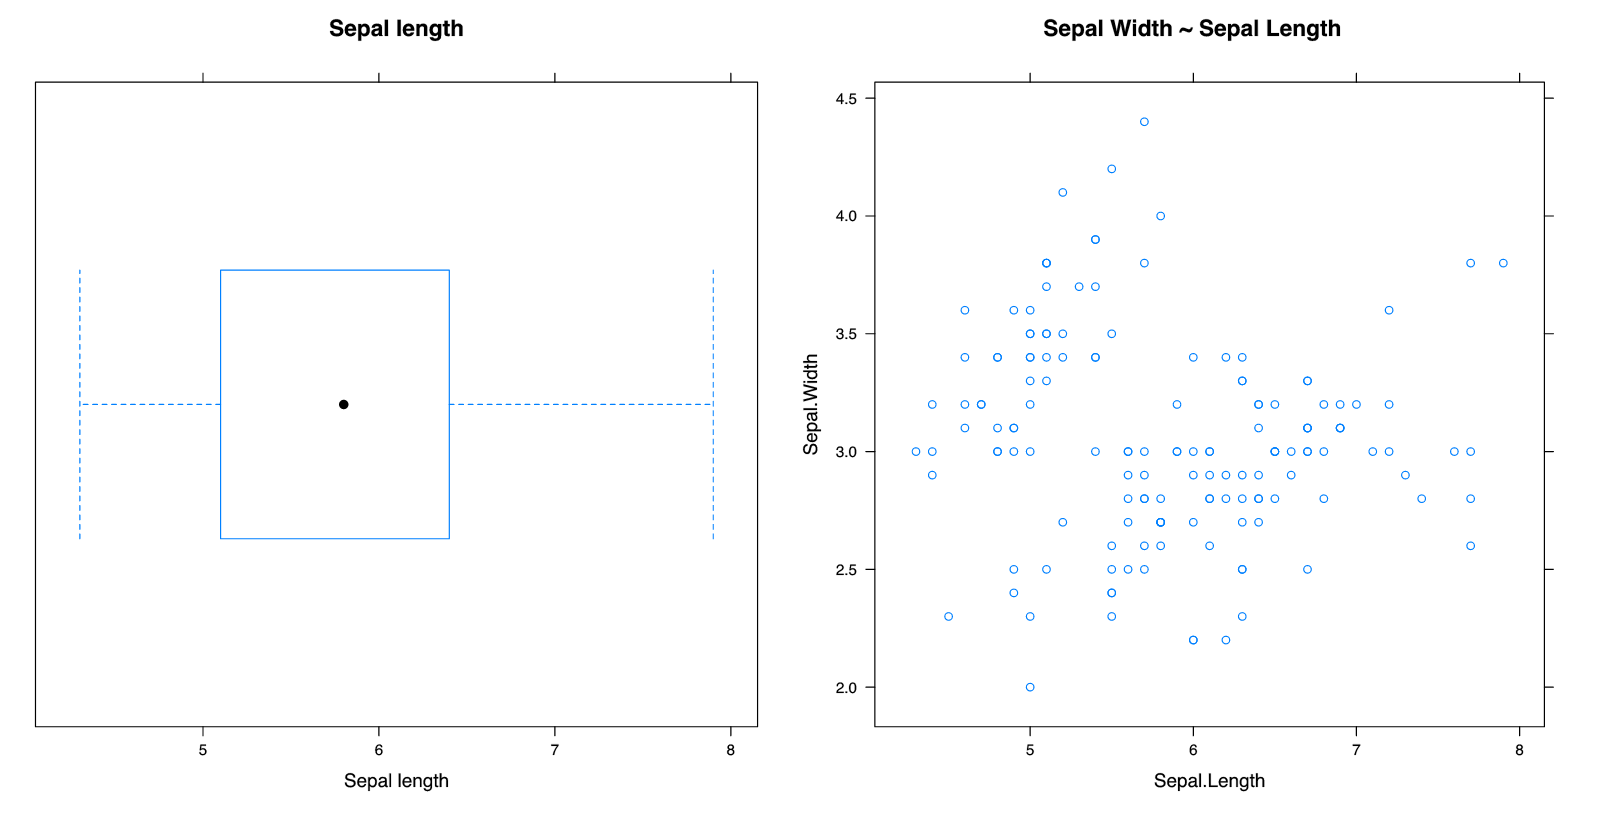
\includegraphics[width=0.7\linewidth,]{./fig/int-bp-2} 

}

\caption{\label{fig:int-bp-2} Boxplot and scatter plot on the same web page}\label{fig:unnamed-chunk-54}
\end{figure}

To highlight the points in the scatterplot that lie in the range of the
box, the user can define the function as follows. We will determine the
indices of the points that lie within the range of the box, and then
pass that index through a function called \texttt{setPoints} to
highlight these in red and group them together in a class called
\texttt{selected}.

\begin{Shaded}
\begin{Highlighting}[]
\NormalTok{highlightPoints <-}\StringTok{ }\ControlFlowTok{function}\NormalTok{(ptr) \{}
  \CommentTok{#identify indices of selected points}
\NormalTok{  index <-}\StringTok{ }\KeywordTok{which}\NormalTok{(}\KeywordTok{min}\NormalTok{(range) }\OperatorTok{<=}\StringTok{ }\NormalTok{iris}\OperatorTok{$}\NormalTok{Sepal.Length}
                 \OperatorTok{&}\StringTok{ }\NormalTok{iris}\OperatorTok{$}\NormalTok{Sepal.Length }\OperatorTok{<=}\StringTok{ }\KeywordTok{max}\NormalTok{(range))}
  \CommentTok{# set identified points to red}
  \KeywordTok{setPoints}\NormalTok{(points,}
            \DataTypeTok{type =} \StringTok{"index"}\NormalTok{,}
            \DataTypeTok{value =}\NormalTok{ index,}
            \DataTypeTok{attrs =} \KeywordTok{list}\NormalTok{(}\DataTypeTok{fill =} \StringTok{"red"}\NormalTok{,}
                         \DataTypeTok{fill.opacity =} \StringTok{"1"}\NormalTok{,}
                         \DataTypeTok{class =} \StringTok{"selected"}\NormalTok{))}
\NormalTok{\}}
\end{Highlighting}
\end{Shaded}

This function can be easily modified by the user and requires them to
make the connection between the data they are dealing with (in this
case, the iris data). As we have defined this interaction, we now need
to define the event that will invoke this interaction before we can send
it to the browser.

\begin{Shaded}
\begin{Highlighting}[]
\NormalTok{boxClick <-}\StringTok{ }\KeywordTok{list}\NormalTok{(}\DataTypeTok{onclick =} \StringTok{'highlightPoints'}\NormalTok{)}
\KeywordTok{addInteractions}\NormalTok{(box, boxClick)}
\end{Highlighting}
\end{Shaded}

We have inserted the function name to run when a `click' is performed
(line 1). Next in the second line of code, we have appended this
interaction to the box element, so that when we click on the box, the
points in the scatterplot that lie within that range should light up in
red. This is shown in \autoref{fig:int-bp-3}.

\begin{figure}[H]

{\centering 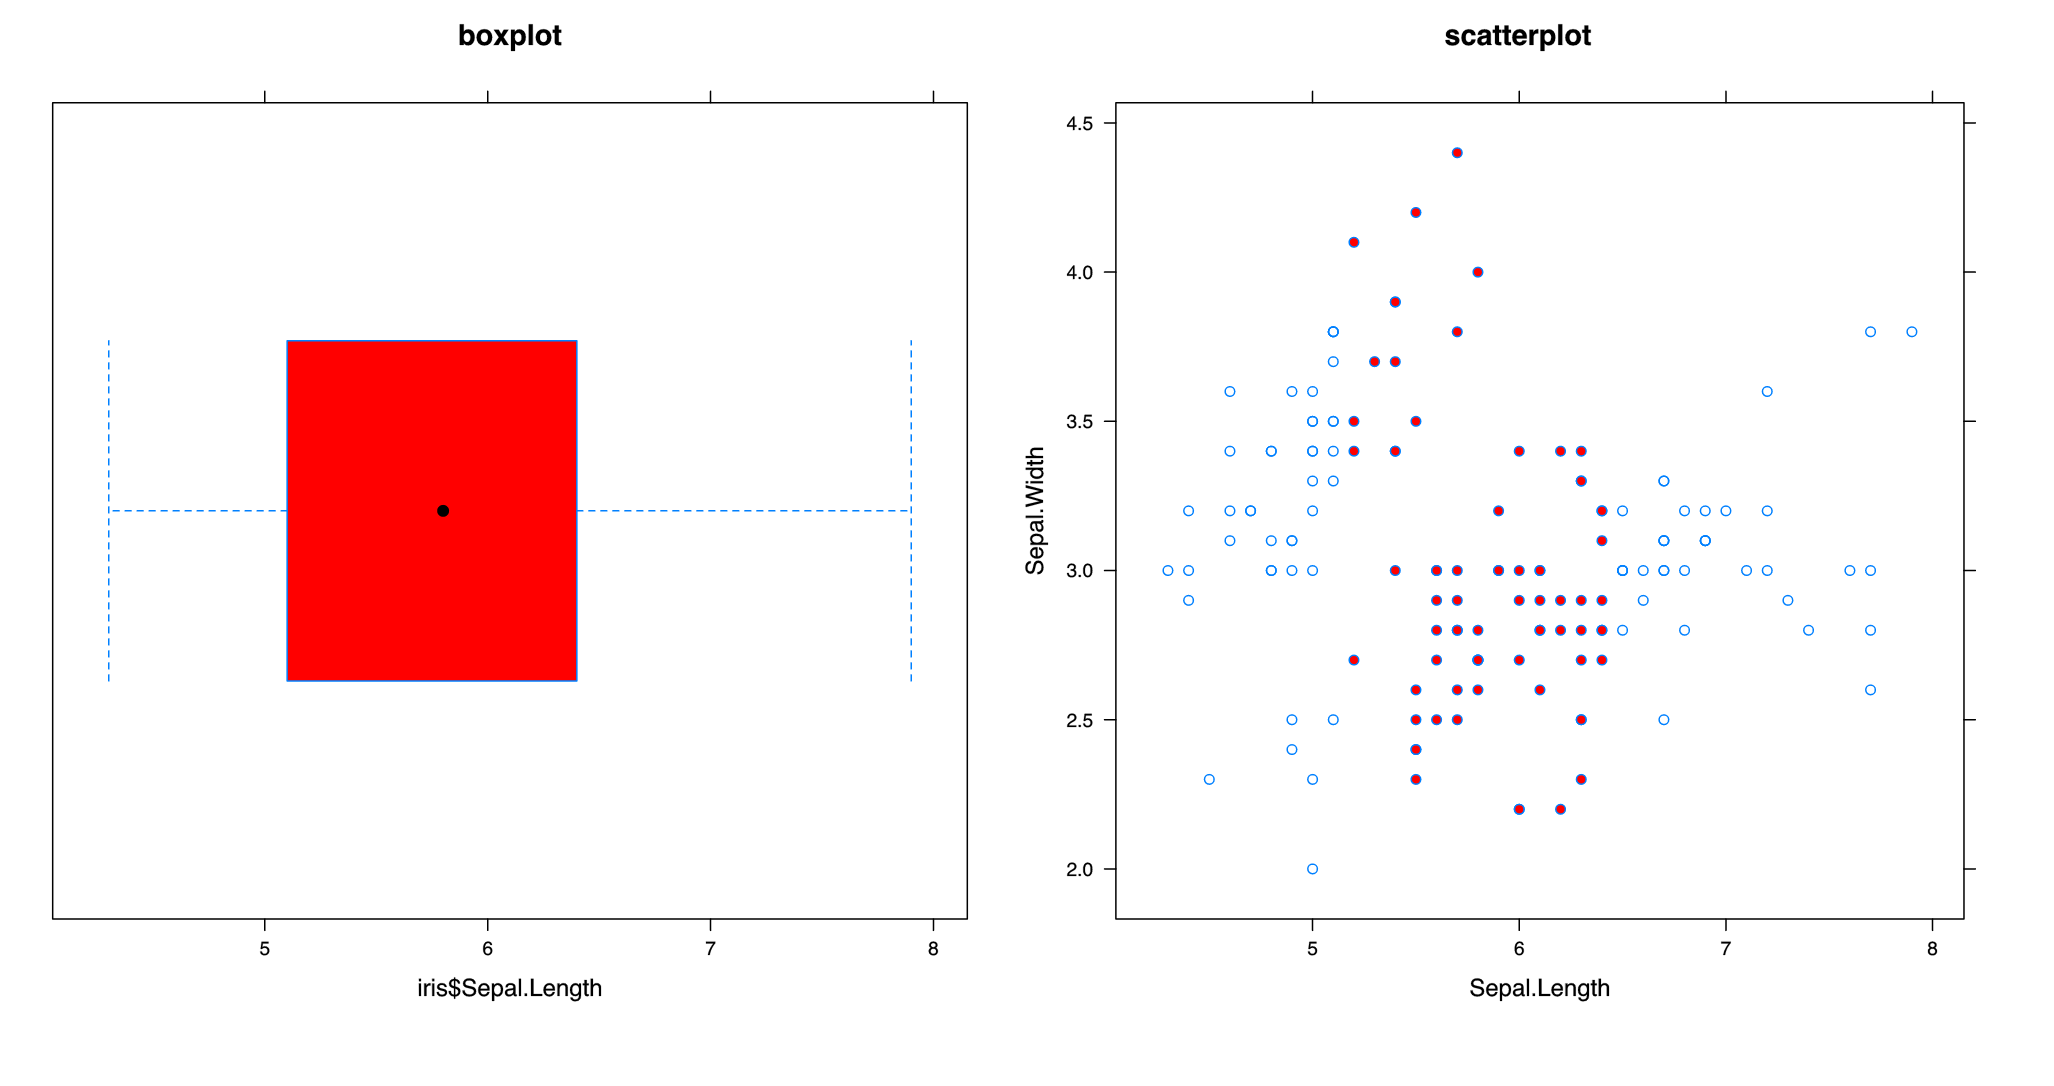
\includegraphics[width=0.7\linewidth,]{./fig/int-bp-3} 

}

\caption{\label{fig:int-bp-3} Click on box plot to light up points on scatter plot}\label{fig:unnamed-chunk-57}
\end{figure}

This example can be further extended by linking the box plot to both a
scatter plot and density plot. Here, we have taken the first 500
observations from a survey conducted with school children in 2009
(CensusAtSchool 2009) and wish to find out the density of girls who have
the heights that lie within that interquartile range of the boys
heights.

We begin by drawing the box plot of boys heights.

First, we draw a box plot of boys heights and attach a hover effect to
the box, similar to what was done previously. The range of the box is
identified for further use.

\begin{Shaded}
\begin{Highlighting}[]
\NormalTok{bw <-}\StringTok{ }\KeywordTok{bwplot}\NormalTok{(boys}\OperatorTok{$}\NormalTok{height, }\DataTypeTok{main =} \StringTok{"Boxplot of boys' heights"}\NormalTok{,}
             \DataTypeTok{xlab =} \StringTok{"Boys' heights (cm)"}\NormalTok{)}
\NormalTok{bw.elements <-}\StringTok{ }\KeywordTok{listElements}\NormalTok{(bw, }\StringTok{"boys_height"}\NormalTok{)}
\NormalTok{box <-}\StringTok{ "boys_height.bwplot.box.polygon.panel.1.1"}
\NormalTok{interactions <-}\StringTok{ }\KeywordTok{list}\NormalTok{(}\DataTypeTok{hover =} \KeywordTok{styleHover}\NormalTok{(}\DataTypeTok{attrs =} \KeywordTok{list}\NormalTok{(}\DataTypeTok{fill =} \StringTok{"red"}\NormalTok{,}
                                                     \DataTypeTok{fill.opacity =} \StringTok{"0.5"}\NormalTok{,}
                                                     \DataTypeTok{pointer.events =} \StringTok{"all"}\NormalTok{)))}
\KeywordTok{draw}\NormalTok{(bw, box, interactions, }\DataTypeTok{new.page =} \OtherTok{TRUE}\NormalTok{)}
\NormalTok{range <-}\StringTok{ }\KeywordTok{returnRange}\NormalTok{(box)}
\end{Highlighting}
\end{Shaded}

Next, we add the scatter plot between boys' heights and armspan to the
page.

\begin{Shaded}
\begin{Highlighting}[]
\NormalTok{sp <-}\StringTok{ }\KeywordTok{xyplot}\NormalTok{(boys}\OperatorTok{$}\NormalTok{armspan }\OperatorTok{~}\StringTok{ }\NormalTok{boys}\OperatorTok{$}\NormalTok{height,}
             \DataTypeTok{main =} \StringTok{"Height vs armspan (boys)"}\NormalTok{,}
             \DataTypeTok{xlab =} \StringTok{"Height(cm)"}\NormalTok{,}
             \DataTypeTok{ylab =} \StringTok{"Armspan"}\NormalTok{)}
\NormalTok{sp.elements <-}\StringTok{ }\KeywordTok{listElements}\NormalTok{(sp, }\StringTok{"sp_bheight"}\NormalTok{)}
\NormalTok{points <-}\StringTok{ "sp_bheight.xyplot.points.panel.1.1"}
\KeywordTok{draw}\NormalTok{(sp)}
\end{Highlighting}
\end{Shaded}

The next line of code adds the density plot of girls heights. Note that
no interactions have been defined yet.

\begin{Shaded}
\begin{Highlighting}[]
\NormalTok{dplot <-}\StringTok{ }\KeywordTok{densityplot}\NormalTok{(}\OperatorTok{~}\NormalTok{girls}\OperatorTok{$}\NormalTok{height,}
                     \DataTypeTok{main=}\StringTok{"Density plot of girl's heights"}\NormalTok{,}
                     \DataTypeTok{xlab=}\StringTok{"Height(cm)"}\NormalTok{)}
\NormalTok{d.elements <-}\StringTok{ }\KeywordTok{listElements}\NormalTok{(dplot, }\StringTok{"girls_height"}\NormalTok{)}
\NormalTok{dlist <-}\StringTok{ }\KeywordTok{list}\NormalTok{(}\DataTypeTok{points =} \StringTok{"girls_height.density.points.panel.1.1"}\NormalTok{,}
              \DataTypeTok{lines =} \StringTok{"girls_height.density.lines.panel.1.1"}\NormalTok{)}
\KeywordTok{draw}\NormalTok{(dplot)}
\end{Highlighting}
\end{Shaded}

\begin{figure}[H]

{\centering 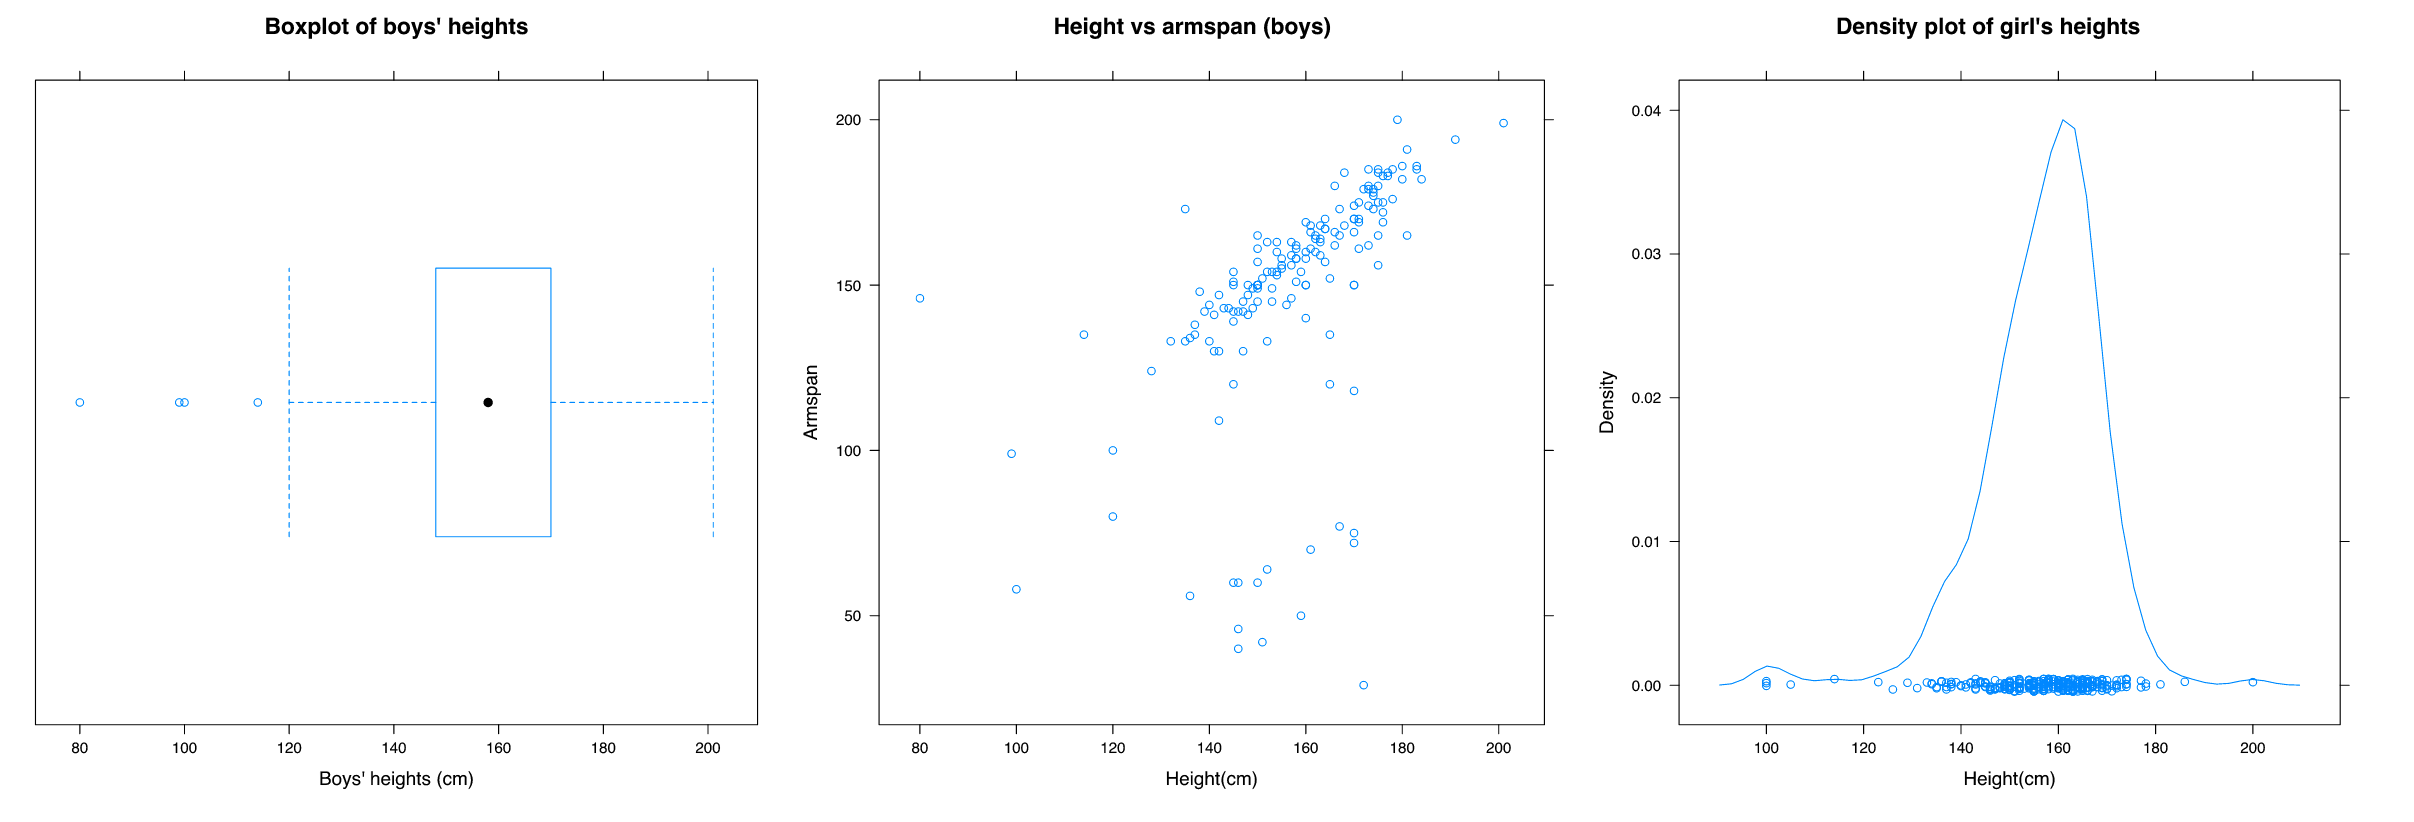
\includegraphics[width=0.7\linewidth,]{./fig/int-bp-4} 

}

\caption{\label{fig:int-bp-4} All three plots on the same web page}\label{fig:unnamed-chunk-62}
\end{figure}

\autoref{fig:int-bp-4} shows all three plots on the same web page.

In order to highlight a certain region of the density plot, we need to
add a new element to the page. This can be done using the
\texttt{addPolygon} function. Ideally, it should be added to the same
group as where the density lines are located. We can use the
\texttt{findPanel} function to identify the correct viewport to attach
to.

\begin{Shaded}
\begin{Highlighting}[]
\CommentTok{# add invisible polygon to the page:}
\NormalTok{panel <-}\StringTok{ }\KeywordTok{findPanel}\NormalTok{(dlist}\OperatorTok{$}\NormalTok{lines)}
\KeywordTok{addPolygon}\NormalTok{(}\StringTok{"highlightRegion"}\NormalTok{, panel, }\DataTypeTok{class =} \StringTok{"highlight"}\NormalTok{,}
           \DataTypeTok{attrs =} \KeywordTok{list}\NormalTok{(}\DataTypeTok{fill =} \StringTok{"red"}\NormalTok{,}
                        \DataTypeTok{stroke =} \StringTok{"red"}\NormalTok{,}
                        \DataTypeTok{stroke.opacity =} \StringTok{"1"}\NormalTok{,}
                        \DataTypeTok{fill.opacity=} \StringTok{"0.5"}\NormalTok{))}
\end{Highlighting}
\end{Shaded}

This polygon will remain invisible to the page as we have not defined
the coordinates of the region. We only want this to appear when the user
has clicked on the box plot.

Next, we write a function that defines what happens after the box plot
is clicked. We identify which the coordinates of the density line lie
within the range of the box plot. This can be used to define the points
of the region that we wish to highlight. We can also highlight the
points in the scatter plot in the same way as we have done in the
previous example.

\begin{Shaded}
\begin{Highlighting}[]
\NormalTok{highlightRange <-}\StringTok{ }\ControlFlowTok{function}\NormalTok{(ptr) \{}

\NormalTok{  coords <-}\StringTok{ }\KeywordTok{returnRange}\NormalTok{(dlist}\OperatorTok{$}\NormalTok{lines)}
\NormalTok{  index <-}\StringTok{ }\KeywordTok{which}\NormalTok{(}\KeywordTok{min}\NormalTok{(range) }\OperatorTok{<=}\StringTok{ }\NormalTok{coords}\OperatorTok{$}\NormalTok{x }\OperatorTok{&}\StringTok{ }\NormalTok{coords}\OperatorTok{$}\NormalTok{x }\OperatorTok{<=}\StringTok{ }\KeywordTok{max}\NormalTok{(range))}
\NormalTok{  xval <-}\StringTok{ }\NormalTok{coords}\OperatorTok{$}\NormalTok{x[index]}
\NormalTok{  yval <-}\StringTok{ }\NormalTok{coords}\OperatorTok{$}\NormalTok{y[index]}

  \CommentTok{# add start and end points for drawing the region to be highlighted}
\NormalTok{  xval <-}\StringTok{ }\KeywordTok{c}\NormalTok{(xval[}\DecValTok{1}\NormalTok{], xval, xval[}\KeywordTok{length}\NormalTok{(xval)])}
\NormalTok{  yval <-}\StringTok{ }\KeywordTok{c}\NormalTok{(}\OperatorTok{-}\DecValTok{1}\NormalTok{, yval, }\OperatorTok{-}\DecValTok{1}\NormalTok{)}

\NormalTok{  pt <-}\StringTok{ }\KeywordTok{convertXY}\NormalTok{(xval, yval, panel)}

  \CommentTok{#set points on added polygon}
  \KeywordTok{setPoints}\NormalTok{(}\StringTok{"highlightRegion"}\NormalTok{, }\DataTypeTok{type =} \StringTok{"coords"}\NormalTok{, }\DataTypeTok{value =}\NormalTok{ pt)}

  \CommentTok{# highlight points on scatter plot, remove missing values}
\NormalTok{  index <-}\StringTok{ }\KeywordTok{which}\NormalTok{(}\KeywordTok{min}\NormalTok{(range) }\OperatorTok{<=}\StringTok{ }\NormalTok{boys}\OperatorTok{$}\NormalTok{height  }
                 \OperatorTok{&}\StringTok{ }\NormalTok{boys}\OperatorTok{$}\NormalTok{height }\OperatorTok{<=}\StringTok{ }\KeywordTok{max}\NormalTok{(range)}
                 \OperatorTok{&}\StringTok{ }\OperatorTok{!}\KeywordTok{is.na}\NormalTok{(boys}\OperatorTok{$}\NormalTok{armspan))}

  \CommentTok{# set points that will highlight according to index}
  \KeywordTok{setPoints}\NormalTok{(points,}
            \DataTypeTok{type =} \StringTok{"index"}\NormalTok{,}
            \DataTypeTok{value =}\NormalTok{ index,}
            \DataTypeTok{attrs =} \KeywordTok{list}\NormalTok{(}\DataTypeTok{fill =} \StringTok{"red"}\NormalTok{,}
                         \DataTypeTok{fill.opacity =} \StringTok{"0.5"}\NormalTok{,}
                         \DataTypeTok{class =} \StringTok{"selected"}\NormalTok{))}

\NormalTok{\}}
\end{Highlighting}
\end{Shaded}

Finally, we define and attach our interactions to the page.

\begin{Shaded}
\begin{Highlighting}[]
\NormalTok{boxClick <-}\StringTok{ }\KeywordTok{list}\NormalTok{(}\DataTypeTok{onclick =} \StringTok{"highlightRange"}\NormalTok{)}
\KeywordTok{addInteractions}\NormalTok{(box, boxClick)}
\end{Highlighting}
\end{Shaded}

When the user now clicks on the box plot, it lights up the points and
the density that lie within that range as seen in
\autoref{fig:int-bp-5}.

\begin{figure}[H]

{\centering 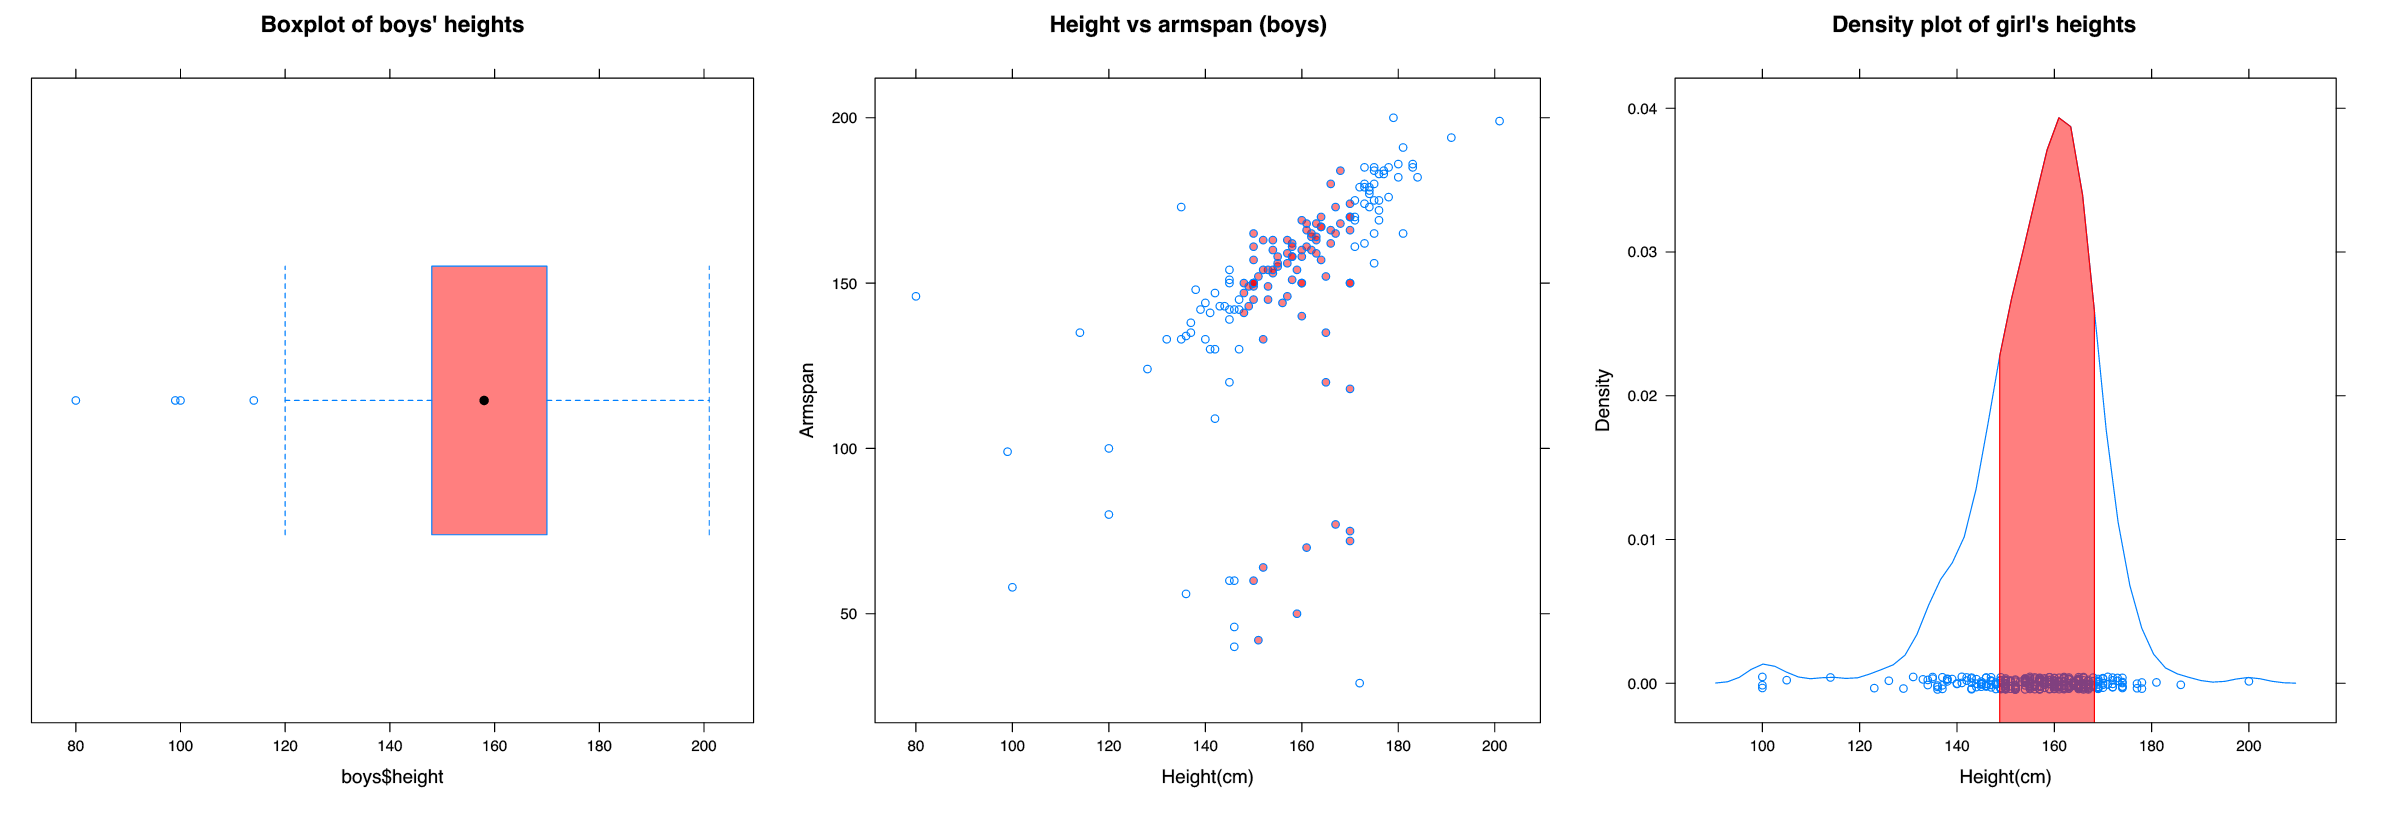
\includegraphics[width=0.7\linewidth,]{./fig/int-bp-5} 

}

\caption{\label{fig:int-bp-5} A single click on the box plot links the density and scatterplot together}\label{fig:unnamed-chunk-66}
\end{figure}

\subsection{Changing the degree of smoothing of a trend
line}\label{changing-the-degree-of-smoothing-of-a-trend-line}

Another example that can be done with \textsf{interactr} is driving an
interaction using a slider. The slider controls the smoothing of the
trend curve. We do not want to redraw the scatter plot when the
smoothing settings change.

Here, it becomes more complex as it requires information to be sent and
queried back and forth between R and the browser.

Once again, we begin by drawing a plot.

\begin{Shaded}
\begin{Highlighting}[]
\NormalTok{iris.plot <-}\StringTok{ }\KeywordTok{xyplot}\NormalTok{(Petal.Length }\OperatorTok{~}\StringTok{ }\NormalTok{Petal.Width,}
                    \DataTypeTok{data =}\NormalTok{ iris,}
                    \DataTypeTok{pch =} \DecValTok{19}\NormalTok{,}
                    \DataTypeTok{type =} \KeywordTok{c}\NormalTok{(}\StringTok{"p"}\NormalTok{, }\StringTok{"smooth"}\NormalTok{),}
                    \DataTypeTok{col.line =} \StringTok{"orange"}\NormalTok{, }\DataTypeTok{lwd =} \DecValTok{3}\NormalTok{)}
\CommentTok{#list elements and print plot}
\KeywordTok{listElements}\NormalTok{(iris.plot)}
\CommentTok{#send plot to browser}
\KeywordTok{draw}\NormalTok{(iris.plot, }\DataTypeTok{new.page =} \OtherTok{TRUE}\NormalTok{)}
\end{Highlighting}
\end{Shaded}

Next, we add a slider to the page. This has not been linked up to any
elements yet (\autoref{fig:int-slider-1}).

\begin{Shaded}
\begin{Highlighting}[]
\CommentTok{#add slider to page:}
\KeywordTok{addSlider}\NormalTok{(}\StringTok{"slider"}\NormalTok{, }\DataTypeTok{min =} \FloatTok{0.5}\NormalTok{, }\DataTypeTok{max =} \DecValTok{1}\NormalTok{, }\DataTypeTok{step =} \FloatTok{0.05}\NormalTok{)}
\end{Highlighting}
\end{Shaded}

\begin{figure}[H]

{\centering 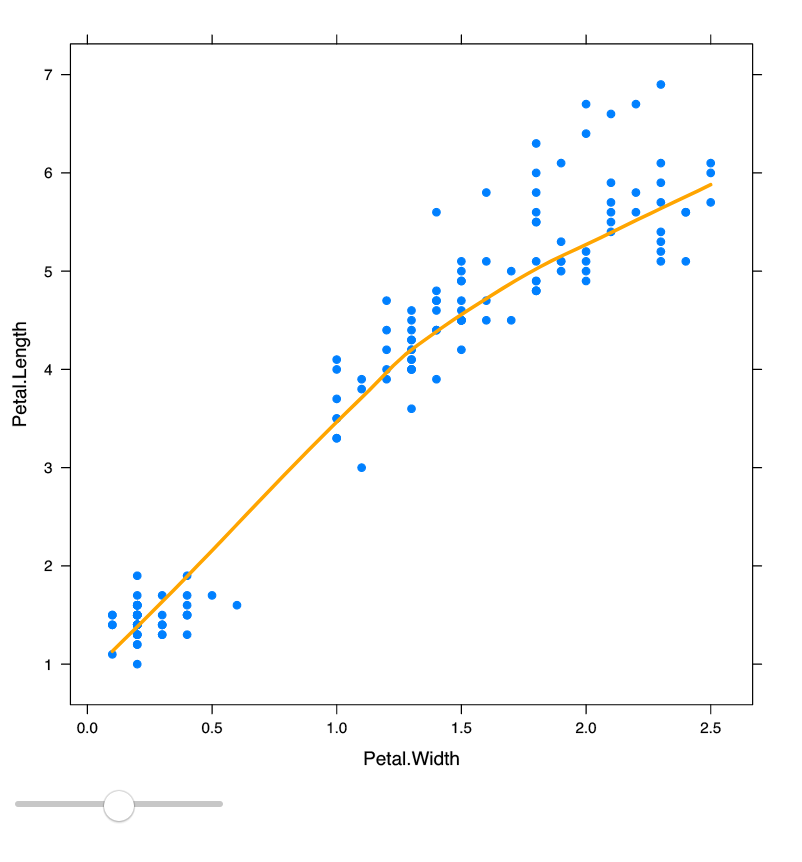
\includegraphics[width=0.7\linewidth,]{./fig/int-slider-1} 

}

\caption{\label{fig:int-slider-1} Plot with slider}\label{fig:unnamed-chunk-69}
\end{figure}

The user can write a function with the argument \texttt{value} to define
what happens when the slider moves. This passes the value of the slider
from the web page back to R. Here, we want to use the value to control
the span of the trend line. To translate the new x and y values of the
points that define the drawn trend line, we need to convert them into
SVG co-ordinates (as mentioned before in Chapter 3.1) before updating
these points.

\begin{Shaded}
\begin{Highlighting}[]
\NormalTok{controlTrendline <-}\StringTok{ }\ControlFlowTok{function}\NormalTok{(value) \{}
  \KeywordTok{showValue}\NormalTok{(value) }\CommentTok{# to show value of the slider}
\NormalTok{  value <-}\StringTok{ }\KeywordTok{as.numeric}\NormalTok{(value)}

  \CommentTok{#user defines what to do next (here, recalculates x and y)}
\NormalTok{  x <-}\StringTok{ }\KeywordTok{seq}\NormalTok{(}\KeywordTok{min}\NormalTok{(iris}\OperatorTok{$}\NormalTok{Petal.Width), }\KeywordTok{max}\NormalTok{(iris}\OperatorTok{$}\NormalTok{Petal.Width), }\DataTypeTok{length =} \DecValTok{20}\NormalTok{)}
\NormalTok{  lo <-}\StringTok{ }\KeywordTok{loess}\NormalTok{(Petal.Length}\OperatorTok{~}\NormalTok{Petal.Width, }\DataTypeTok{data =}\NormalTok{ iris, }\DataTypeTok{span =}\NormalTok{ value)}
\NormalTok{  y <-}\StringTok{ }\KeywordTok{predict}\NormalTok{(lo, x)}

  \CommentTok{#convert coordinates and set points}
\NormalTok{  panel <-}\StringTok{ }\KeywordTok{findPanel}\NormalTok{(}\StringTok{'plot_01.xyplot.points.panel.1.1'}\NormalTok{)}
\NormalTok{  pt <-}\StringTok{ }\KeywordTok{convertXY}\NormalTok{(x, y, panel)}
  \KeywordTok{setPoints}\NormalTok{(}\StringTok{"plot_01.loess.lines.panel.1.1"}\NormalTok{, }\DataTypeTok{type =} \StringTok{"coords"}\NormalTok{, }\DataTypeTok{value =}\NormalTok{ pt)}
\NormalTok{\}}
\end{Highlighting}
\end{Shaded}

Once this is done, we need to pass this function to retrieve the value
of the slider as it moves. To do this, have a special function called
\texttt{sliderCallback}. This redefines and creates the entire function
that is now called \texttt{sliderValue}.

\begin{Shaded}
\begin{Highlighting}[]
\CommentTok{# pass defined function through sliderCallback to pass slider value correctly}
\NormalTok{sliderValue <-}\StringTok{ }\KeywordTok{sliderCallback}\NormalTok{(controlTrendline)}
\end{Highlighting}
\end{Shaded}

Finally, we can link the \texttt{sliderValue} function back to the
slider such that when the slider moves, the trend line will be updated
based upon the value of the slider as seen in
\autoref{fig:int-slider-2}.

\begin{Shaded}
\begin{Highlighting}[]
\NormalTok{int <-}\StringTok{ }\KeywordTok{list}\NormalTok{(}\DataTypeTok{oninput =} \StringTok{"sliderValue"}\NormalTok{)}
\KeywordTok{addInteractions}\NormalTok{(}\StringTok{"slider"}\NormalTok{, int)}
\end{Highlighting}
\end{Shaded}

\begin{figure}[H]

{\centering 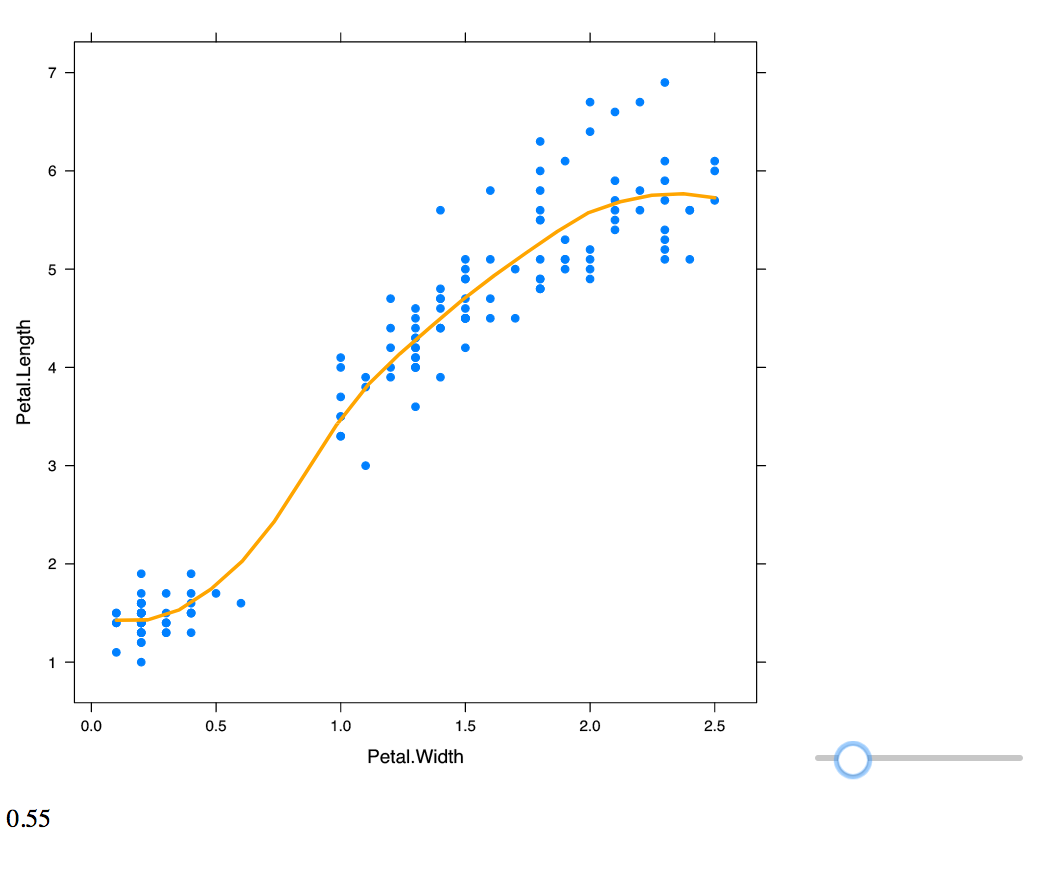
\includegraphics[width=0.7\linewidth,]{./fig/int-slider-2} 

}

\caption{\label{fig:int-slider-2} Plot with slider that controls the smoothness of the trend line}\label{fig:unnamed-chunk-73}
\end{figure}

Another feature that the user may want to achieve is to be able to
select a set of points and compute a trend line using those specific
points. To be able to do this, we need to add a new element to the page
to represent this special trend line. This can be done using the
\texttt{addLine} function. Here, we have added it to the same group
where these points are.

\begin{Shaded}
\begin{Highlighting}[]
\NormalTok{pointsPanel <-}\StringTok{ }\KeywordTok{findPanel}\NormalTok{(}\StringTok{"plot_01.xyplot.points.panel.1.1"}\NormalTok{)}
\KeywordTok{addLine}\NormalTok{(}\StringTok{"newSmooth"}\NormalTok{, pointsPanel, }\DataTypeTok{class =} \StringTok{"hello"}\NormalTok{, }\KeywordTok{list}\NormalTok{(}\DataTypeTok{stroke =} \StringTok{"red"}\NormalTok{,}
                                                  \DataTypeTok{stroke.width =} \StringTok{"1"}\NormalTok{,}
                                                  \DataTypeTok{fill =} \StringTok{"none"}\NormalTok{))}
\end{Highlighting}
\end{Shaded}

Note that this appears to be hidden on the page, as the points of this
line have not been defined yet. Next, a new function needs to be defined
to be able to compute this new smoother.

\begin{Shaded}
\begin{Highlighting}[]
\CommentTok{#create new smoother:}
\NormalTok{createSmooth  =}\StringTok{ }\ControlFlowTok{function}\NormalTok{(index) \{}
  \CommentTok{#this returns the indices of the points selected}
\NormalTok{  index <-}\StringTok{ }\KeywordTok{as.numeric}\NormalTok{(}\KeywordTok{unlist}\NormalTok{(}\KeywordTok{strsplit}\NormalTok{(index, }\StringTok{","}\NormalTok{)))}
  \CommentTok{#filter selected points:}
  \ControlFlowTok{if}\NormalTok{ (}\KeywordTok{length}\NormalTok{(index) }\OperatorTok{>}\StringTok{ }\DecValTok{20}\NormalTok{) \{}
\NormalTok{    selected <-}\StringTok{ }\NormalTok{iris[index, ]}
\NormalTok{    x <-}\StringTok{ }\KeywordTok{seq}\NormalTok{(}\KeywordTok{min}\NormalTok{(selected}\OperatorTok{$}\NormalTok{Petal.Width), }\KeywordTok{max}\NormalTok{(selected}\OperatorTok{$}\NormalTok{Petal.Width), }\DataTypeTok{length =} \DecValTok{20}\NormalTok{)}
\NormalTok{    lo <<-}\StringTok{ }\KeywordTok{loess}\NormalTok{(Petal.Length }\OperatorTok{~}\NormalTok{Petal.Width, }\DataTypeTok{data =}\NormalTok{ selected, }\DataTypeTok{span =} \DecValTok{1}\NormalTok{)}
\NormalTok{    y <-}\StringTok{ }\KeywordTok{predict}\NormalTok{(lo, x)}
    \CommentTok{#convert co-ordinates:}
\NormalTok{    pt <-}\StringTok{ }\KeywordTok{convertXY}\NormalTok{(x, y, pointsPanel)}
\NormalTok{  \} }\ControlFlowTok{else}\NormalTok{ \{}
\NormalTok{    pt <-}\StringTok{ ""}
\NormalTok{  \}}
  \KeywordTok{setPoints}\NormalTok{(}\StringTok{"newSmooth"}\NormalTok{, }\DataTypeTok{type =} \StringTok{"coords"}\NormalTok{, }\DataTypeTok{value =}\NormalTok{ pt)}
\NormalTok{\}}
\end{Highlighting}
\end{Shaded}

Because the index of the points need to be returned from the browser
back to R, we use \texttt{boxCallback} to help us link these functions
together. As linking a selection box is a special type of interaction,
we can pass our defined function through to the \texttt{addSelectionBox}
function which adds on the selection box and links it together to
compute the new smoother.

\begin{Shaded}
\begin{Highlighting}[]
\CommentTok{#link callback functions together to pass index values to function}
\NormalTok{boxIndex =}\StringTok{ }\KeywordTok{boxCallback}\NormalTok{(createSmooth)}
\KeywordTok{addSelectionBox}\NormalTok{(}\DataTypeTok{plotNum =} \DecValTok{1}\NormalTok{, }\DataTypeTok{el =} \StringTok{"plot_01.xyplot.points.panel.1.1"}\NormalTok{, }\DataTypeTok{f =} \StringTok{"boxIndex"}\NormalTok{)}
\end{Highlighting}
\end{Shaded}

\begin{figure}[H]

{\centering 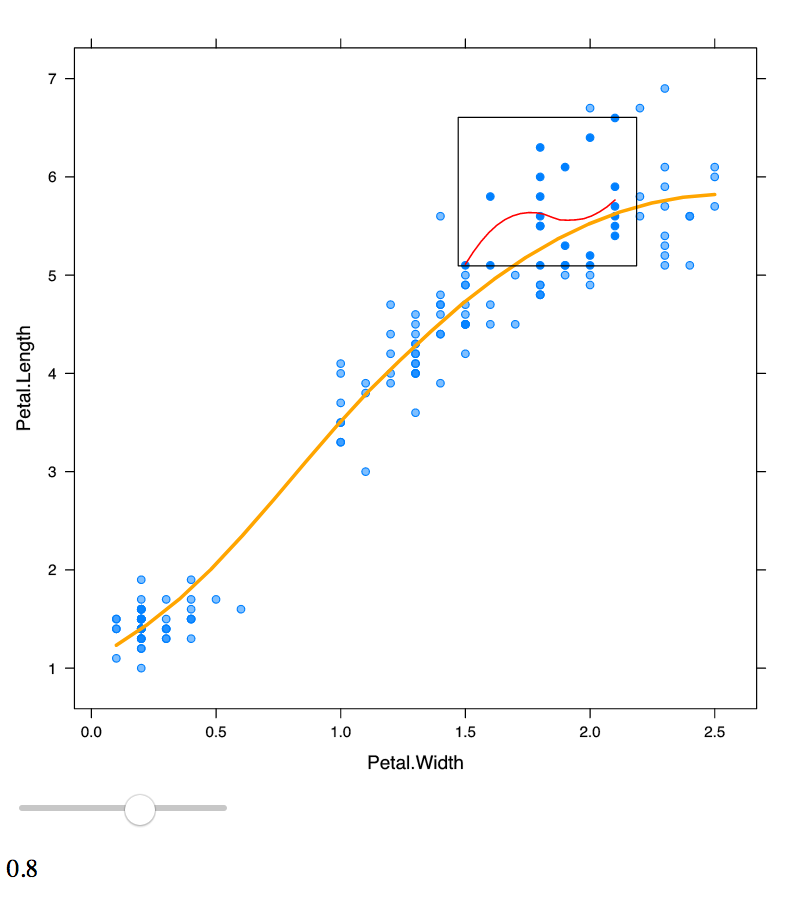
\includegraphics[width=0.7\linewidth,]{./fig/int-slider-3} 

}

\caption{\label{fig:int-slider-3} Plot that has a selection box feature that draws a separate smoother}\label{fig:unnamed-chunk-77}
\end{figure}

The user now can draw a selection box over a set of points, and a new
smoother should render on the page based upon these points (shown in
\autoref{fig:int-slider-3}).

The notion of having special functions is required when there is a need
for querying the browser for more information (such as the value of the
slider, or the points selected on a page). In the box plot example in
Section 4.2.1, the information was stored back in R which did not
require a special callback function. These types of interactions are
more complex to handle.

\section{Compatibility with other graphics
systems}\label{compatibility-with-other-graphics-systems}

A useful feature of interactr is its compatibility with other R graphing
systems including \textsf{lattice}, \textsf{graphics} (also known as
base R plots), and \textsf{ggplot2}.

Before we begin, we will briefly mention the two different graphics
systems in R. One is known as the \textsf{graphics}, the other known as
\textsf{grid} . A major difference between the two systems is that
\textsf{grid} is not made to draw complete plots by a single function
(Murrell 2011). Rather, it is seen as a lower level graphics tool that
has been used to build successful higher level plotting packages,
including lattice and ggplot2. Packages that are built on top of the
\textsf{grid} system can be accessible to the other \textsf{grid} tools
available, including \textsf{gridSVG} and \textsf{grImport} (Murrell
2011). Likewise, there are other tools that are only compatible with the
\textsf{graphics} system. There are many other packages that are built
on top of these two major systems that make up the graphics that we can
produce in R.

The examples discussed so far with \textsf{interactr} have been done
with \textsf{lattice} plots. However, it is possible to achieve the same
with other plotting systems. To demonstrate, we have taken the box plot
example in \autoref{fig:int-bp-3} and replicated it using
\textsf{graphics} and \textsf{ggplot2}.

\subsection{graphics plots}\label{graphics-plots}

As briefly mentioned in Chapter 3, in order to convert SVG objects using
gridSVG the objects must be grid objects. In the case of graphics plots,
we cannot directly call gridSVG to convert it into an SVG. A simple
solution to this is to use the \textsf{gridGraphics} package (Murrell
2015), which acts as a translator by converting graphics plots into grid
plots with a consistent naming scheme. The \texttt{grid.echo()} function
achieves this.

\begin{Shaded}
\begin{Highlighting}[]
\KeywordTok{library}\NormalTok{(grid)}
\KeywordTok{plot}\NormalTok{(}\DecValTok{1}\OperatorTok{:}\DecValTok{10}\NormalTok{, }\DecValTok{1}\OperatorTok{:}\DecValTok{10}\NormalTok{)}
\KeywordTok{grid.ls}\NormalTok{()}
\NormalTok{gridGraphics}\OperatorTok{::}\KeywordTok{grid.echo}\NormalTok{()}
\KeywordTok{grid.ls}\NormalTok{()}
\end{Highlighting}
\end{Shaded}

\begin{figure}[H]

{\centering 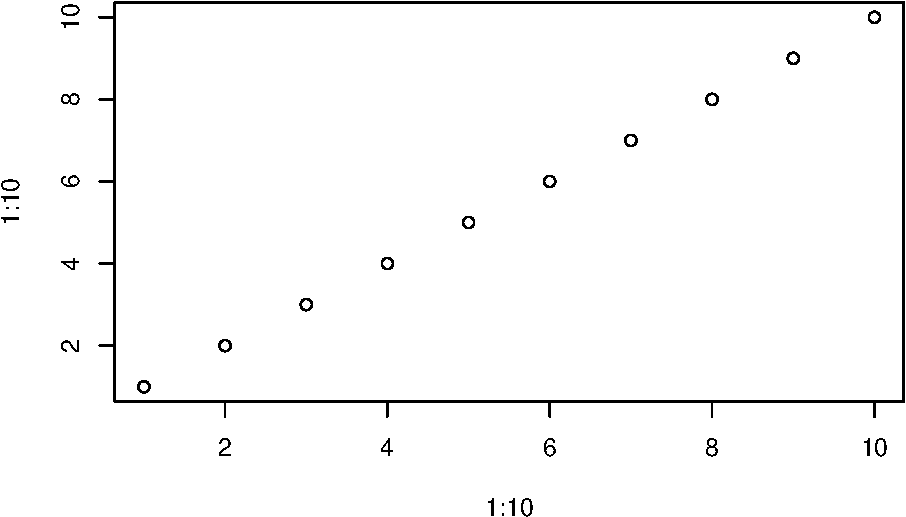
\includegraphics{figures/unnamed-chunk-79-1} 

}

\caption{\label{fig:gg-convert} An example of a graphics plot that is converted into a grid plot using gridGraphics}\label{fig:unnamed-chunk-791}
\end{figure}

\begin{figure}[H]

{\centering 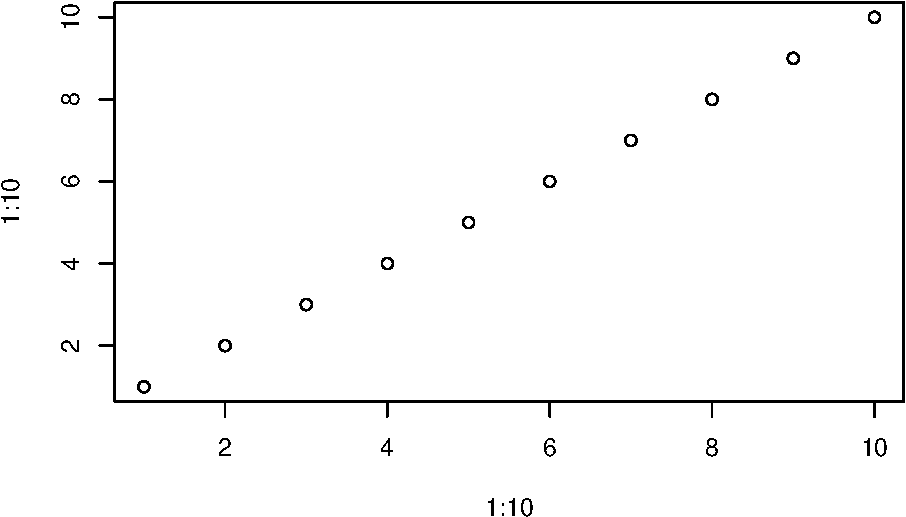
\includegraphics{figures/unnamed-chunk-79-2} 

}

\caption{\label{fig:gg-convert} An example of a graphics plot that is converted into a grid plot using gridGraphics}\label{fig:unnamed-chunk-792}
\end{figure}

\begin{verbatim}
## graphics-plot-1-points-1
## graphics-plot-1-bottom-axis-line-1
## graphics-plot-1-bottom-axis-ticks-1
## graphics-plot-1-bottom-axis-labels-1
## graphics-plot-1-left-axis-line-1
## graphics-plot-1-left-axis-ticks-1
## graphics-plot-1-left-axis-labels-1
## graphics-plot-1-box-1
## graphics-plot-1-xlab-1
## graphics-plot-1-ylab-1
\end{verbatim}

The code above produces a graphics plot that has been converted to a
grid plot (as seen in \autoref{fig:gg-convert}). To check this, we have
called \texttt{grid.ls()} to check whether is a grid object. In the
first call, it returns nothing because it is not a grid object. Once we
call \texttt{grid.echo()}, \texttt{grid.ls()} returns a list of elements
that make up the plot.

Another problem is that when we plot or try save it into a variable, it
does not plot to the graphics device. To solve this, we can use
\texttt{recordPlot} to record the plot that has been drawn to further
process it (Paul Murrell and Allaire 2015).

The only change that we need to do is run an extra \texttt{recordPlot}
command before we call \texttt{listElements}.

Once again, we begin by drawing the plot. We then record the plot before
listing its elements. This will automatically convert the plot using
\texttt{grid.echo()}.

\begin{Shaded}
\begin{Highlighting}[]
\KeywordTok{boxplot}\NormalTok{(iris}\OperatorTok{$}\NormalTok{Sepal.Length, }\DataTypeTok{horizontal =} \OtherTok{TRUE}\NormalTok{)}
\NormalTok{pl <-}\StringTok{ }\KeywordTok{recordPlot}\NormalTok{()}
\KeywordTok{listElements}\NormalTok{(pl)}
\end{Highlighting}
\end{Shaded}

Next, the same process occurs. We see that the code is very similar to
what was done previously with \texttt{lattice}. We can use the same
\protect\hyperlink{highlightPoints}{\texttt{highlightPoints}} function
defined back in the \texttt{lattice} example.

\begin{Shaded}
\begin{Highlighting}[]
\CommentTok{# identify box in box plot and send the plot to the browser}
\NormalTok{box =}\StringTok{ "graphics-plot-1-polygon-1"}
\NormalTok{interactions <-}\StringTok{ }\KeywordTok{list}\NormalTok{(}\DataTypeTok{hover =} \KeywordTok{styleHover}\NormalTok{(}\DataTypeTok{attrs =} \KeywordTok{list}\NormalTok{(}\DataTypeTok{fill =} \StringTok{"red"}\NormalTok{,}
                                                     \DataTypeTok{fill.opacity =} \StringTok{"1"}\NormalTok{)))}
\KeywordTok{draw}\NormalTok{(pl, box, interactions, }\DataTypeTok{new.page =} \OtherTok{TRUE}\NormalTok{)}
\NormalTok{range <-}\StringTok{ }\KeywordTok{returnRange}\NormalTok{(box)}

\CommentTok{# plot a graphics scatter plot}
\KeywordTok{plot}\NormalTok{(iris}\OperatorTok{$}\NormalTok{Sepal.Length, iris}\OperatorTok{$}\NormalTok{Sepal.Width)}
\NormalTok{sp <-}\StringTok{ }\KeywordTok{recordPlot}\NormalTok{()}
\KeywordTok{listElements}\NormalTok{(sp)}
\KeywordTok{draw}\NormalTok{(sp)}

\CommentTok{#add interactions}
\NormalTok{points <-}\StringTok{ 'graphics-plot-1-points-1'}
\NormalTok{boxClick <-}\StringTok{ }\KeywordTok{list}\NormalTok{(}\DataTypeTok{onclick =} \StringTok{"highlightPoints"}\NormalTok{)}
\KeywordTok{addInteractions}\NormalTok{(box, boxClick)}
\end{Highlighting}
\end{Shaded}

\begin{figure}[H]

{\centering 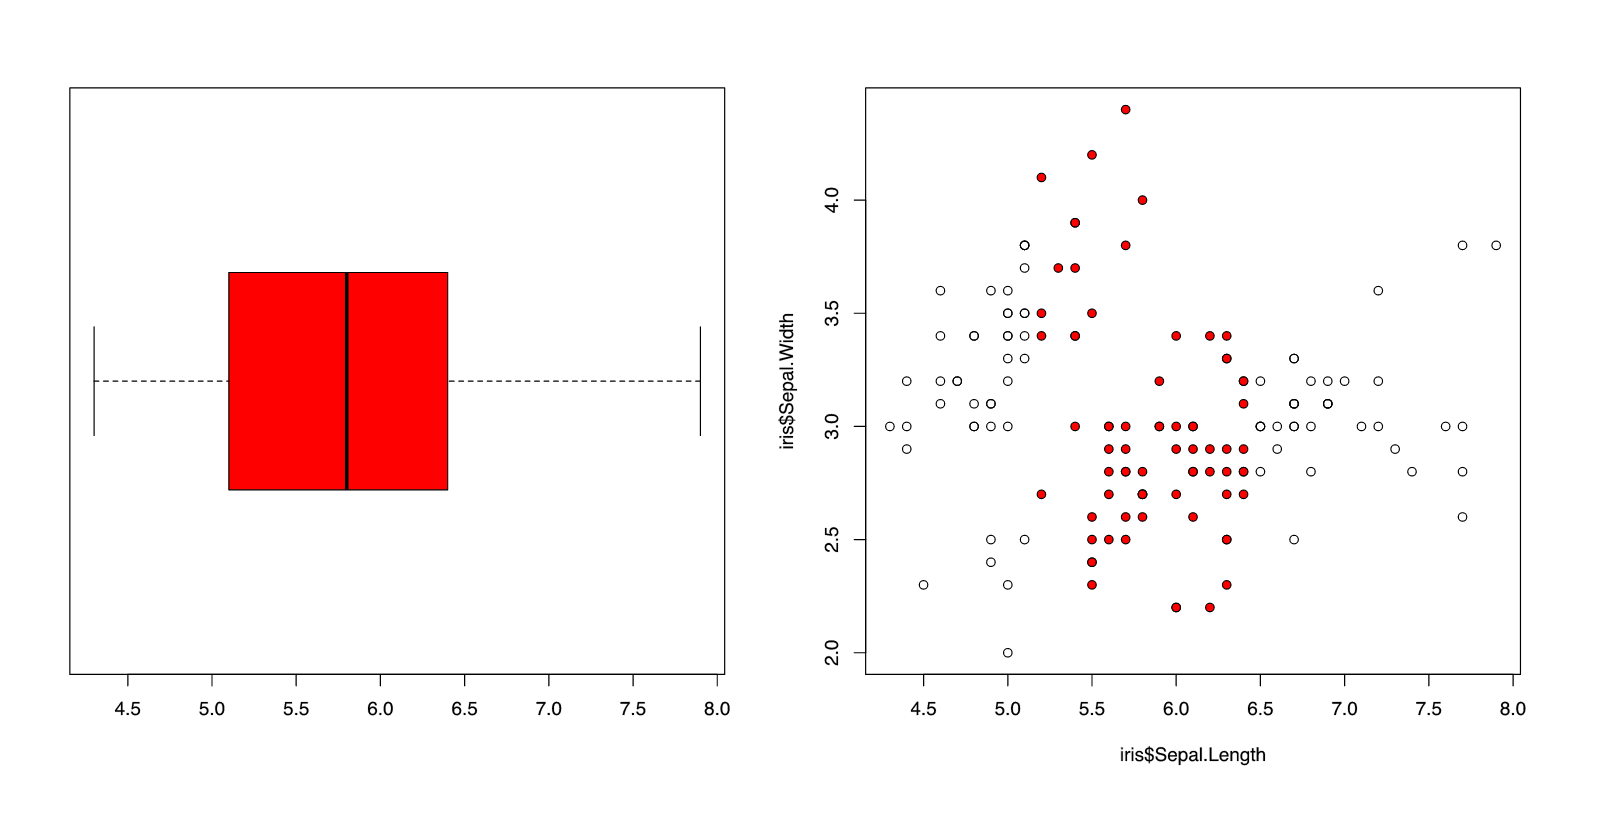
\includegraphics[width=0.7\linewidth,]{./fig/int-bp-graphics} 

}

\caption{\label{fig:int-bp-graphics} Box plot example replicated using a graphics plot}\label{fig:unnamed-chunk-82}
\end{figure}

The same interaction has been achieved in \autoref{int-bp-graphics}.
This shows that there is potential for customising interactions onto
graphics plots. The process is the same, except for an additional step
to convert a \textsf{graphics} plot into a \textsf{grid} type plot.

\subsection{ggplot2}\label{ggplot2}

\textsf{ggplot2} (Wickham 2009) is a popular plotting system in R based
upon the ``Grammar of Graphics''. It is built upon the \textsf{grid}
graphics system, which makes it compatible with \textsf{gridSVG}.

\begin{Shaded}
\begin{Highlighting}[]
\KeywordTok{library}\NormalTok{(ggplot2)}
\NormalTok{p <-}\StringTok{ }\KeywordTok{ggplot}\NormalTok{(}\DataTypeTok{data =}\NormalTok{ iris, }\KeywordTok{aes}\NormalTok{(}\DataTypeTok{x =} \StringTok{""}\NormalTok{, }\DataTypeTok{y =}\NormalTok{ Sepal.Length)) }\OperatorTok{+}\StringTok{ }\KeywordTok{geom_boxplot}\NormalTok{()}
\NormalTok{p.elements <-}\StringTok{ }\KeywordTok{listElements}\NormalTok{(p)}
\NormalTok{box <-}\StringTok{ }\KeywordTok{findElement}\NormalTok{(}\StringTok{"geom_polygon.polygon"}\NormalTok{)}
\NormalTok{interactions <-}\StringTok{ }\KeywordTok{list}\NormalTok{(}\DataTypeTok{hover =} \KeywordTok{styleHover}\NormalTok{(}\DataTypeTok{attrs =} \KeywordTok{list}\NormalTok{(}\DataTypeTok{fill =} \StringTok{"red"}\NormalTok{,}
                                                     \DataTypeTok{fill.opacity =} \StringTok{"1"}\NormalTok{,}
                                                     \DataTypeTok{pointer.events =} \StringTok{"all"}\NormalTok{)))}
\KeywordTok{draw}\NormalTok{(p, box, interactions, }\DataTypeTok{new.page =} \OtherTok{TRUE}\NormalTok{)}
\end{Highlighting}
\end{Shaded}

However, because it works on a completely different co-ordinates system,
we cannot simply use the \texttt{returnRange} function to define the
range of the box.

The native coordinates given by \textsf{grid} do not return that data
coordinates of the ggplot. A simple solution to this is that the
information about the plot can be extracted from \texttt{ggplot\_build}.
Below, we have manually identified the range of the box.

\begin{Shaded}
\begin{Highlighting}[]
\CommentTok{# find the range of the box:}
\NormalTok{boxData <-}\StringTok{ }\KeywordTok{ggplot_build}\NormalTok{(p)}\OperatorTok{$}\NormalTok{data[[}\DecValTok{1}\NormalTok{]]}
\CommentTok{# for a box plot - IQR: lower, upper}
\NormalTok{range <-}\StringTok{ }\KeywordTok{c}\NormalTok{(boxData}\OperatorTok{$}\NormalTok{lower, boxData}\OperatorTok{$}\NormalTok{upper)}
\end{Highlighting}
\end{Shaded}

Next, we add the scatterplot to the page.

\begin{Shaded}
\begin{Highlighting}[]
\NormalTok{sp <-}\StringTok{ }\KeywordTok{ggplot}\NormalTok{(}\DataTypeTok{data =}\NormalTok{ iris, }\KeywordTok{aes}\NormalTok{(}\DataTypeTok{x =}\NormalTok{ Sepal.Width, }\DataTypeTok{y =}\NormalTok{Sepal.Length)) }\OperatorTok{+}\StringTok{ }\KeywordTok{geom_point}\NormalTok{()}
\NormalTok{sp.elements <-}\StringTok{ }\KeywordTok{listElements}\NormalTok{(sp)}
\KeywordTok{draw}\NormalTok{(sp)}
\end{Highlighting}
\end{Shaded}

The difference is the naming of these grid elements do not have a clear
structure in \textsf{ggplot2}. To locate the points on the plot, we can
use \texttt{findElement} to return the element corresponding to these
points.

\begin{Shaded}
\begin{Highlighting}[]
\NormalTok{points <-}\StringTok{ }\KeywordTok{findElement}\NormalTok{(}\StringTok{"geom_point.point"}\NormalTok{)}
\end{Highlighting}
\end{Shaded}

Next, we can use the same function
\protect\hyperlink{highlightPoints}{\texttt{highlightPoints}} defined
before sending these interactions to the browser
(\autoref{fig:int-bp-ggplot2}).

\begin{Shaded}
\begin{Highlighting}[]
\CommentTok{#using highlightPoints defined previously in 3.1}
\NormalTok{boxClick <-}\StringTok{ }\KeywordTok{list}\NormalTok{(}\DataTypeTok{onclick =} \StringTok{"highlightPoints"}\NormalTok{)}
\KeywordTok{addInteractions}\NormalTok{(box, boxClick)}
\end{Highlighting}
\end{Shaded}

\begin{figure}[H]

{\centering 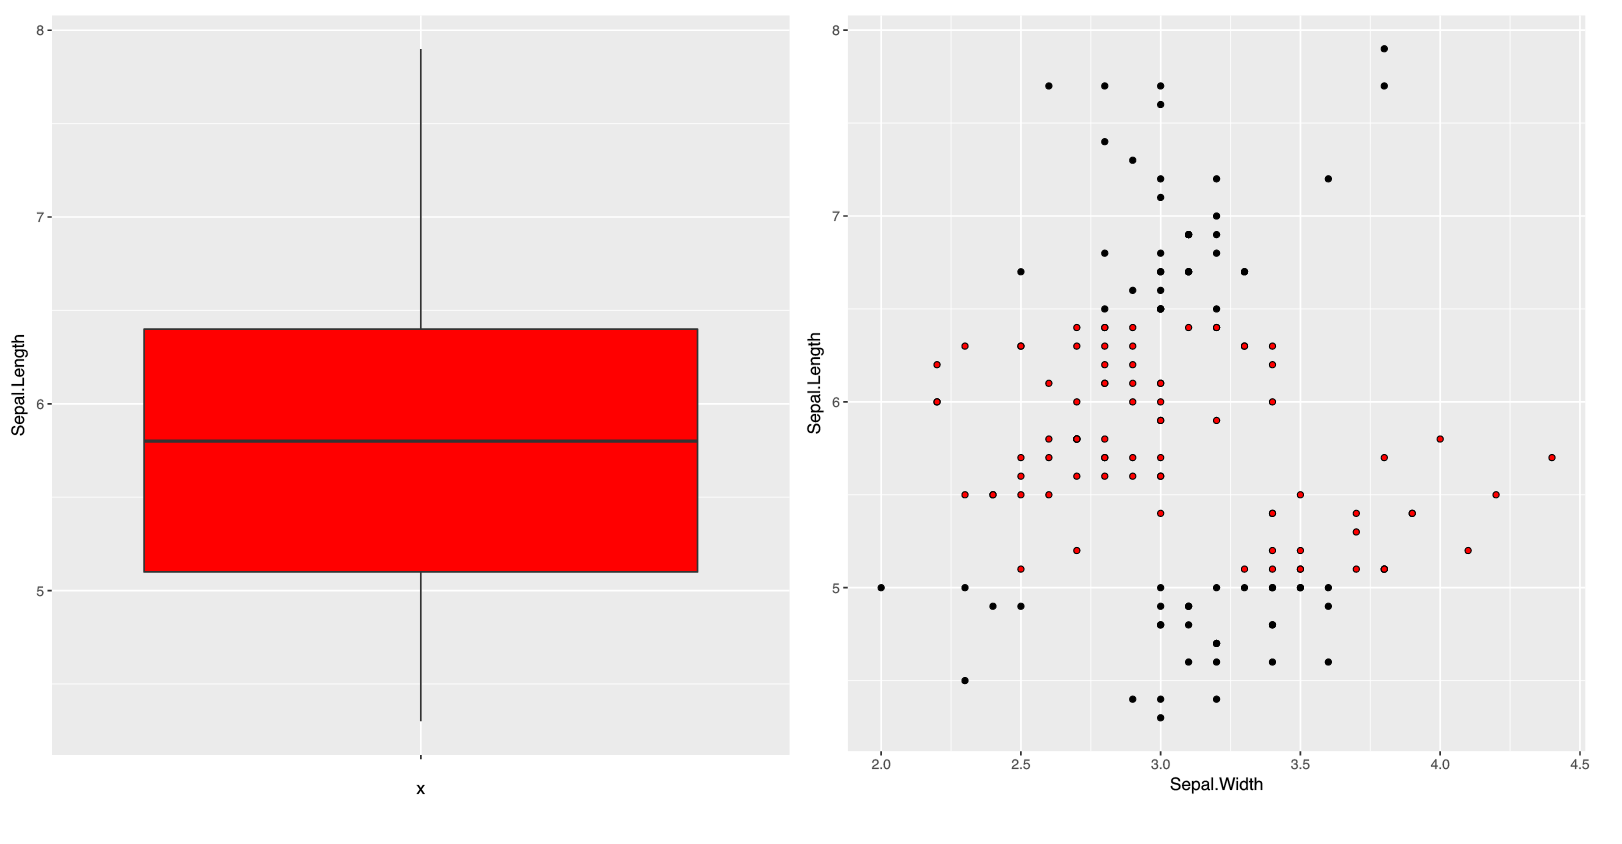
\includegraphics[width=0.7\linewidth,]{./fig/int-bp-ggplot2} 

}

\caption{\label{fig:int-bp-ggplot2} Box plot example replicated using a plot rendered with ggplot2}\label{fig:unnamed-chunk-88}
\end{figure}

This demonstrates that there is a possible way of achieving interactions
with \textsf{ggplot2} and that there is potential for \textsf{interactr}
to plug into different R plotting systems. Consequently, when we assess
the compatibility of different plotting systems, we need to take into
account of possible detours that could occur. Because this is a
simplistic example, it may become more complex when we try to achieve
more sophisticated interactions.

The \textsf{interactr} package acts as a proof-of-concept and a starting
point for what aims to be a general solution for adding simple
interactions to plots generated in R. There is potential in plugging
into different plotting systems, however it depends on how compatible
these systems are with the underlying tools of the \textsf{interactr}
package. But the most commonly used systems are covered by our examples.
The process is based upon defining what you want to draw in R,
identifying elements drawn, and defining specific interactions to attach
to certain elements drawn that can be viewed in a web browser. Next, we
discuss the limitations and future directions of using this process as a
way of creating web interactive graphics.

\newpage

\chapter{Discussion}\label{discussion}

The \textsf{interactr} package provides a way of generating simple
interactive R plots that can be viewed in a web browser. It is
advantageous in the sense that we can define and customise interactions
with flexibility. It can also achieve unidirectional linking between
plots. However, there are many limitations present with its current
implementation and is not yet recommended for general use. But it does
have potential to be further developed in the future. In this section we
will discuss the advantages \protect\hyperlink{advantages}{(Section
5.1)} and limitations of this method
\protect\hyperlink{limitations}{(Section 5.2)}, further compare it to
existing tools \protect\hyperlink{comparison-to-existing-tools}{(Section
5.3)}, and briefly comment on future directions for developing
\textsf{interactr}.

\hypertarget{advantages}{\section{Advantages}\label{advantages}}

The idea of \textsf{interactr} is inspired from finding a more easier
way to customise certain interactions onto plots drawn in R without the
need to learn JavaScript. It takes advantage of R's flexible graphics
system and caters for both \textsf{graphics} and \textsf{grid} plots.

Using the \textsf{DOM} package allows us to use R to recompute and do
calculations that originally cannot be done in JavaScript, such as
recomputing densities on a plot based upon a selection. Below is an
example of changing density plots based upon what the user has selected
(\autoref{fig:int-density}).

\begin{figure}[H]

{\centering 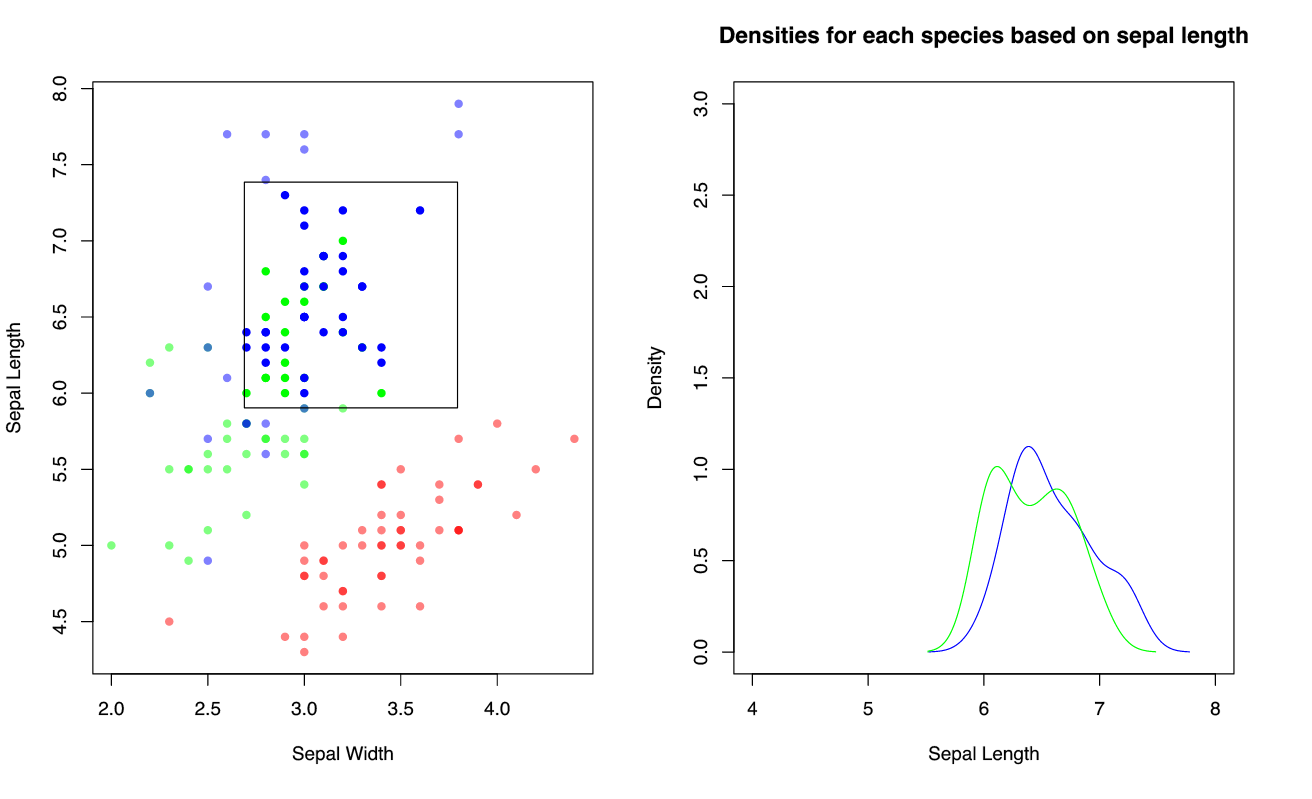
\includegraphics[width=18.22in,]{./fig/int-density-example} 

}

\caption{\label{fig:int-density} Different selections (left) recompute different densities (right) with interactr}\label{fig:unnamed-chunk-89}
\end{figure}

This cannot be done with any of the existing tools unless paired with
\textsf{shiny}. However, shiny simply reproduces the plot each time.
Using an asynchronous system like \textsf{DOM} also creates a more
responsive application.

The main advantage for identifying graphical elements to data is that we
have more flexibility in targeting sub components of a plot. A prime
example of an interaction that is difficult to implement across other
tools is linking a part of the box plot to other plots (seen in Section
4.2.1).

Another advantage is that we are able to add layers on top of plots and
draw shapes that can help provide more information. This cannot be
easily done by the existing tools as it requires information on how
these plots are layered and rendered. With \textsf{gridSVG} underneath
to provide a clear mapping structure of these layers, we can add on
elements to existing plots on the web page to show more about a user's
interaction such as a selection or a click. They can also be used to
highlight regions and draw new elements. The is exemplified in the trend
line example in Section 4.2.2, where an additional smoother can be added
to the plot.

\textsf{interactr} can be used to create links between plots via clicks
and selection boxes, where a single plot can control the rest of the
plots. It may be possible to create multi-directional links, but becomes
more complex to co-ordinate. It is a success in its own for providing
basic interactions to any type of plot drawn in R. However, there are
still many limitations that are present with its current implementation.

\hypertarget{limitations}{\section{Limitations}\label{limitations}}

With \textsf{gridSVG}, one major limitation is that only \textsf{grid}
objects can be converted into SVG. This limits us to plots that must be
drawn in R to a graphics device before it can be sent to the browser. A
further limitation is that \textsf{gridSVG} is relatively slow when we
try to convert a plot made up of many elements. Currently, work is
proceeding to make \textsf{gridSVG} faster.

Because \textsf{interactr} is mainly built upon the \textsf{DOM}
package, many of the limitations of \textsf{DOM} highlighted in Section
3.2 are carried over. Applications made with \textsf{DOM} are generated
for a single user in a single session only. Furthermore, because the
\textsf{DOM} package is still under development, it cannot be used for
production purposes yet. Just as \textsf{shiny} applications require a
\textsf{shiny} server for them to be hosted on the web, \textsf{DOM}
would require something similar to allow for applications to be shared
and accessed. A few trials using a \textsf{shiny} server have been
successful, but these only act as a provisional solution. Furthermore,
because the underlying system involving requests being sent between R
and the web browser, this can be slower than plots that are driven fully
by JavaScript.

There are further limitations with its current implementation. The
approach is based upon the graphical elements produced. This requires
the user to be able to link the particular elements of the data which is
more tedious than the existing tools discussed in Section 2 that link
data to graphical elements on the page. The user must call
\texttt{listElements} before sending the plot to the browser as it
prints the plot to a current device and returns a list of elements that
make up the plot. This is crucial for plotting systems that do not have
a consistent naming scheme. If we reprint the plot, the tags will
constantly change which may cause a mismatch between element matching
between the plot on the web and the plot in R. This occurs with
\textsf{ggplot2}, where if we re-plot with the exact same command, the
names of these elements change every time. Another problem with using
\texttt{listElements} is that the user will need to deduce which element
corresponds to what is seen on the plot as the naming for these objects
in by these plotting systems may not be clear. If it is a plot that is
made directly from \textsf{grid} where the user has named everything
clearly, then this is not a problem. The code below shows the difference
between the naming scheme in lattice and \textsf{ggplot2}.

Listing the elements from a plot produced with lattice:

\begin{Shaded}
\begin{Highlighting}[]
\NormalTok{sp <-}\StringTok{ }\KeywordTok{xyplot}\NormalTok{(Petal.Length }\OperatorTok{~}\StringTok{ }\NormalTok{Petal.Width, }\DataTypeTok{data =}\NormalTok{ iris)}
\KeywordTok{listElements}\NormalTok{(sp)}
\end{Highlighting}
\end{Shaded}

\begin{center}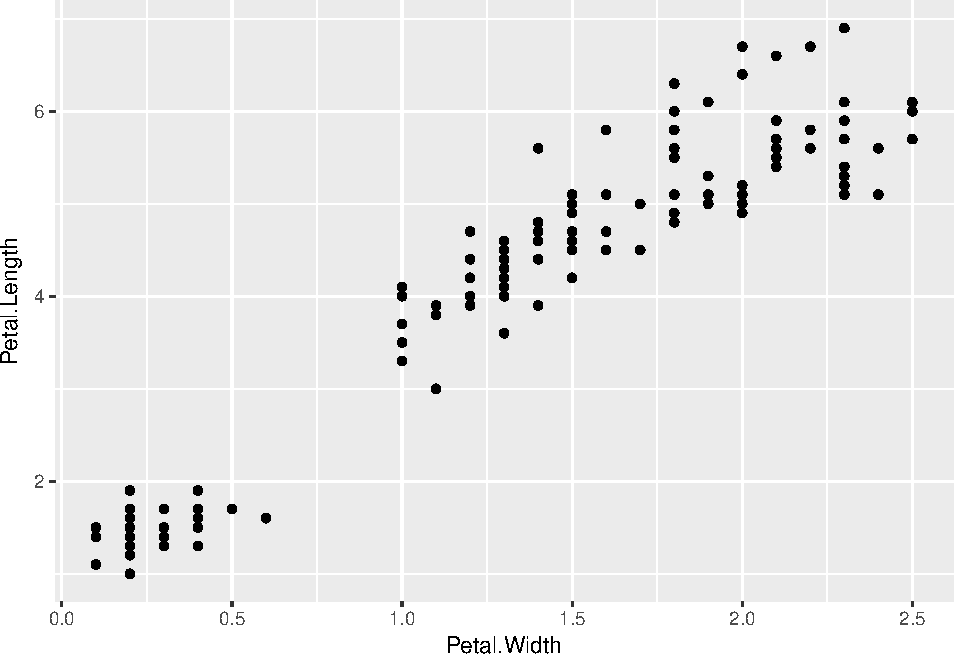
\includegraphics{figures/unnamed-chunk-90-1} \end{center}

\begin{verbatim}
## plot_01.background
## plot_01.xlab
## plot_01.ylab
## plot_01.ticks.top.panel.1.1
## plot_01.ticks.left.panel.1.1
## plot_01.ticklabels.left.panel.1.1
## plot_01.ticks.bottom.panel.1.1
## plot_01.ticklabels.bottom.panel.1.1
## plot_01.ticks.right.panel.1.1
## plot_01.xyplot.points.panel.1.1
## plot_01.border.panel.1.1
\end{verbatim}

Listing the elements from a plot produced with \textsf{ggplot2}:

\begin{Shaded}
\begin{Highlighting}[]
\NormalTok{p <-}\StringTok{ }\KeywordTok{ggplot}\NormalTok{(iris) }\OperatorTok{+}\StringTok{ }\KeywordTok{aes}\NormalTok{(}\DataTypeTok{x =}\NormalTok{ Petal.Width, }\DataTypeTok{y =}\NormalTok{ Petal.Length) }\OperatorTok{+}\StringTok{ }\KeywordTok{geom_point}\NormalTok{()}
\KeywordTok{listElements}\NormalTok{(p)}
\end{Highlighting}
\end{Shaded}

\begin{center}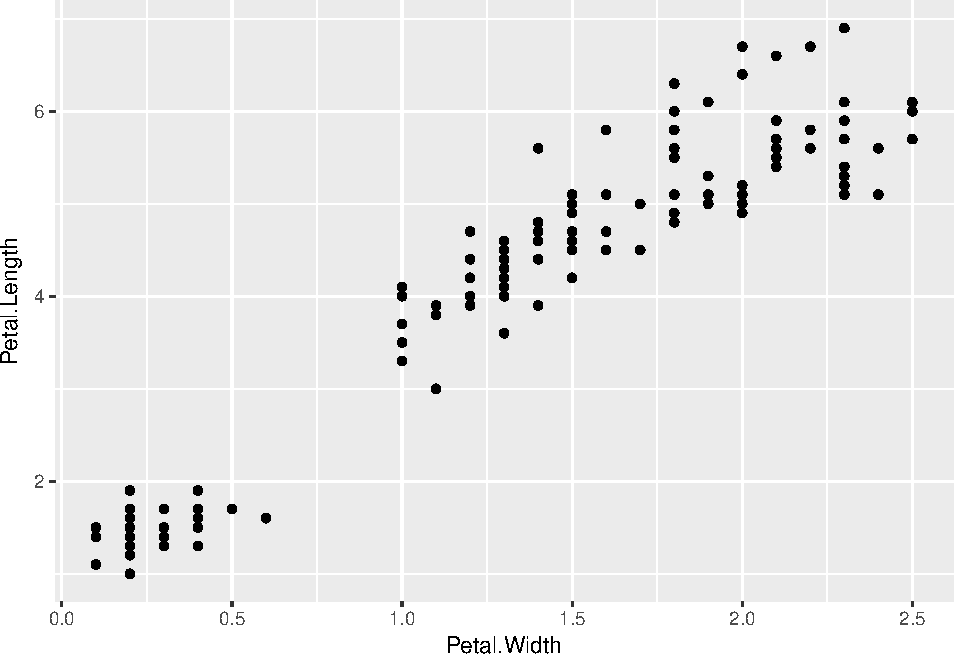
\includegraphics{figures/unnamed-chunk-91-1} \end{center}

\begin{verbatim}
## layout
##   background.1-7-10-1
##   panel.6-4-6-4
##     grill.gTree.829
##       panel.background..rect.820
##       panel.grid.minor.y..polyline.822
##       panel.grid.minor.x..polyline.824
##       panel.grid.major.y..polyline.826
##       panel.grid.major.x..polyline.828
##     NULL
##     geom_point.points.816
##     NULL
##     panel.border..zeroGrob.817
##   spacer.7-5-7-5
##   spacer.7-3-7-3
##   spacer.5-5-5-5
##   spacer.5-3-5-3
##   axis-t.5-4-5-4
##   axis-l.6-3-6-3
##     axis.line.y..zeroGrob.848
##     axis
##       axis.1-1-1-1
##         GRID.text.845
##       axis.1-2-1-2
##   axis-r.6-5-6-5
##   axis-b.7-4-7-4
##     axis.line.x..zeroGrob.841
##     axis
##       axis.1-1-1-1
##       axis.2-1-2-1
##         GRID.text.838
##   xlab-t.4-4-4-4
##   xlab-b.8-4-8-4
##     GRID.text.832
##   ylab-l.6-2-6-2
##     GRID.text.835
##   ylab-r.6-6-6-6
##   subtitle.3-4-3-4
##   title.2-4-2-4
##   caption.9-4-9-4
\end{verbatim}

Another limitation is the number of interactions that can be attached.
So far, the examples expressed in Section 4.3 require a single element
to be controlled and assumes that the each grid object listed
corresponds to a single SVG element. We can attach many interactions and
events to a single element at a time, but not many elements to many
different interactions at once. There is a need for a more flexible
system when dealing with multiple interactions for achieving more
complex interactions. Furthermore, only one kind of interaction can be
expressed for a single event. This means that the function created by
the user must be fully defined in a single function rather than multiple
functions. For example, if a hover requires both adding a tooltip and to
turn the element red, then this would need to be written as a single
function as we can only attach one to each event.

Code must also be written in a certain order to work. Plots in R must be
drawn to a graphics device before being sent to the browser, while a new
web page must be set up before we can start adding elements and
interactions to the page. These devices must still be open in order to
communicate and retrieve existing information about the plot. In cases
of dealing with multiple plots, one of the disadvantages is that we lose
information about the previous plot in R. This means that the user is
required to identify what kind of information they need to extract
before they move onto the next plot. This is demonstrated in the example
in section 4.2.1 of linking a box plot to other plots together. Before
the user can move onto the scatter plot, the range of the box and
viewports were stored in order to be used in the defined function. This
means that we cannot jump back and forth between plots. A possible
solution to this is to store the information about each plot that is
sent to the web browser so that it can be retrieved by the user if
needed in R. Another approach would be to plot all necessary plots in a
single window which would eliminate the need for this.

A further assumption that the \textsf{interactr} package currently has
is that the \texttt{native} units in textsf\{grid\} represent the data
values that are plotted. As discussed in Section 4.3.2, \textsf{ggplot2}
uses a different co-ordinate system and this assumption does not hold.
Instead, we need to take a detour and get the data values that are
stored in \texttt{ggplot\_build()}.

\hypertarget{comparison-to-existing-tools}{\section{Comparison to
existing tools}\label{comparison-to-existing-tools}}

\textsf{interactr}`s main point of difference is the ability to
replicate plots or objects drawn in R (in both graphics systems) and to
achieve on-plot and off-plot interactivity. \textsf{shiny} can do this
but you cannot easily attach specific interactions as the whole plot is
rendered as a single raster image file (such as a png). Furthermore,
many of these existing tools rely on the \textsf{shiny} framework. As
highlighted in Section 2.3, one of the major disadvantages that
\textsf{shiny} possesses is a tendency to recompute and redraw entire
plots whenever an input changes. In \textsf{interactr}, only the part of
the plot that the user specifically targets is modified and customised
interactions can be achieved. It provides a possible way of linking
different types of plots together, whereas existing tools, specifically
crosstalk, have focused on linked brushing between 'row-observation'
data. To put this in perspective, the simple example of linking box
plots to other types of plots in Figure 4.2 is an interaction that is
difficult to achieve without expert knowledge of their respective APIs.

In comparison to the existing tools discussed in Section 2,
\textsf{interactr} has a more complex API for users. The main reason for
this is to increase flexibility across creating different types of
interactions. But this is entirely developmental. In comparison to using
\textsf{DOM} and \textsf{gridSVG} directly, it provides convenience for
certain processes, such as drawing an SVG plot and adding elements to
the web page and styling hovers. Currently, only certain interactions
highlighted in Section 4.2 can be achieved.

There is potential for designing a more simpler and structured API that
is more intuitive for developers and users. An example to highlight this
is changing the bandwidth of a density plot (shown below with
\textsf{interactr} in \autoref{fig:d1}). This example has been
replicated with \textsf{ggvis}(\autoref{fig:d2}),
\textsf{shiny}(\autoref{fig:d3}), and with \textsf{plotly+shiny}
(\autoref{fig:d4}). The \textsf{animint} package will not be able to do
this because it is restricted to clicks and selection.

\begin{figure}[H]

{\centering 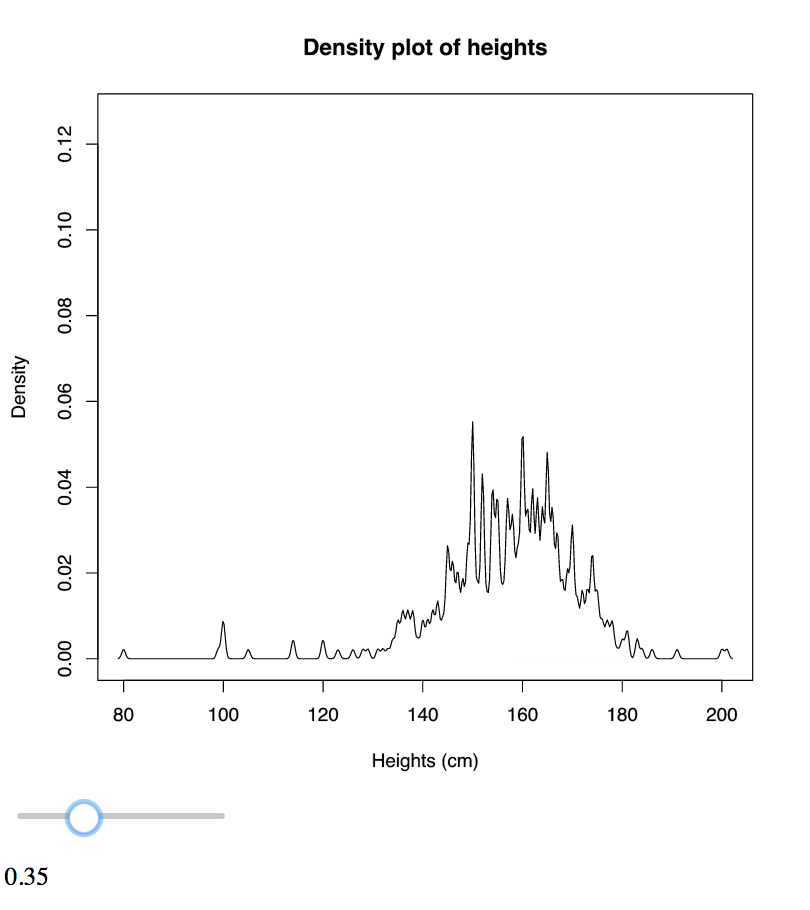
\includegraphics[width=11.25in,]{./fig/interactr-density} 

}

\caption{\label{fig:d1} control density bandwidth with interactr}\label{fig:unnamed-chunk-92}
\end{figure}

\begin{figure}[H]

{\centering 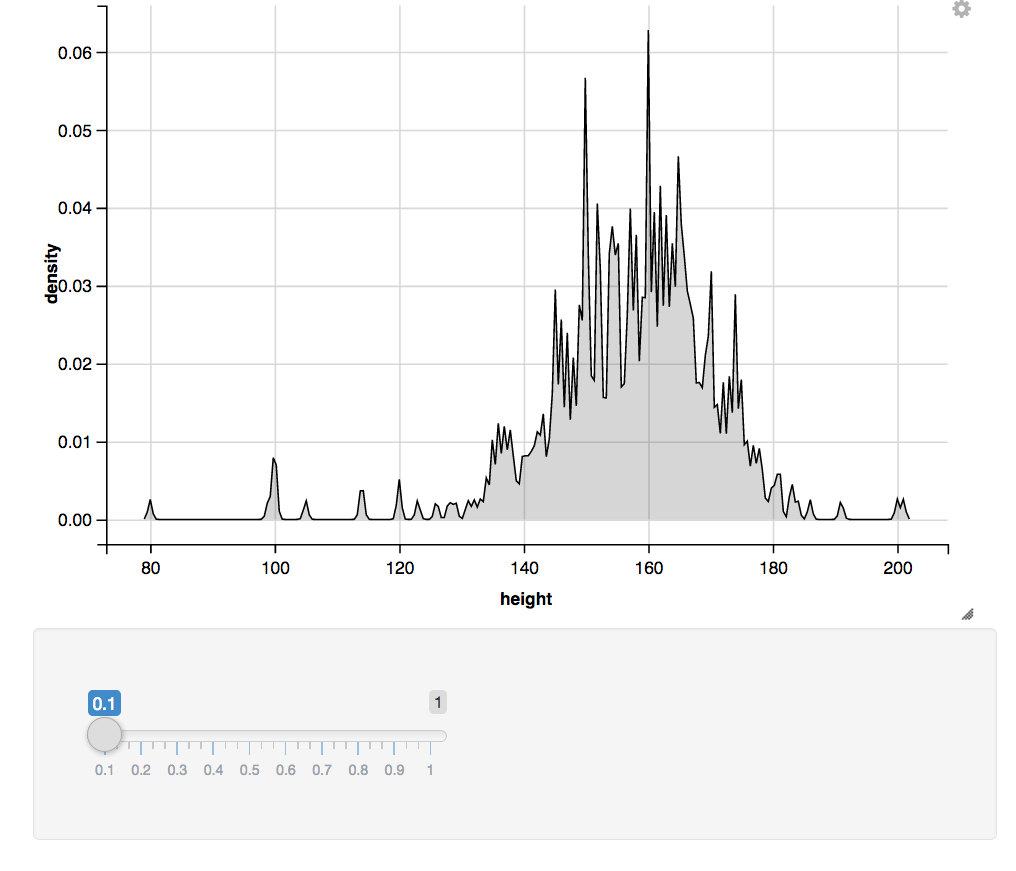
\includegraphics[width=14.11in,]{./fig/ggvis-density} 

}

\caption{\label{fig:d2} control density bandwidth with ggvis}\label{fig:unnamed-chunk-93}
\end{figure}

\begin{figure}[H]

{\centering 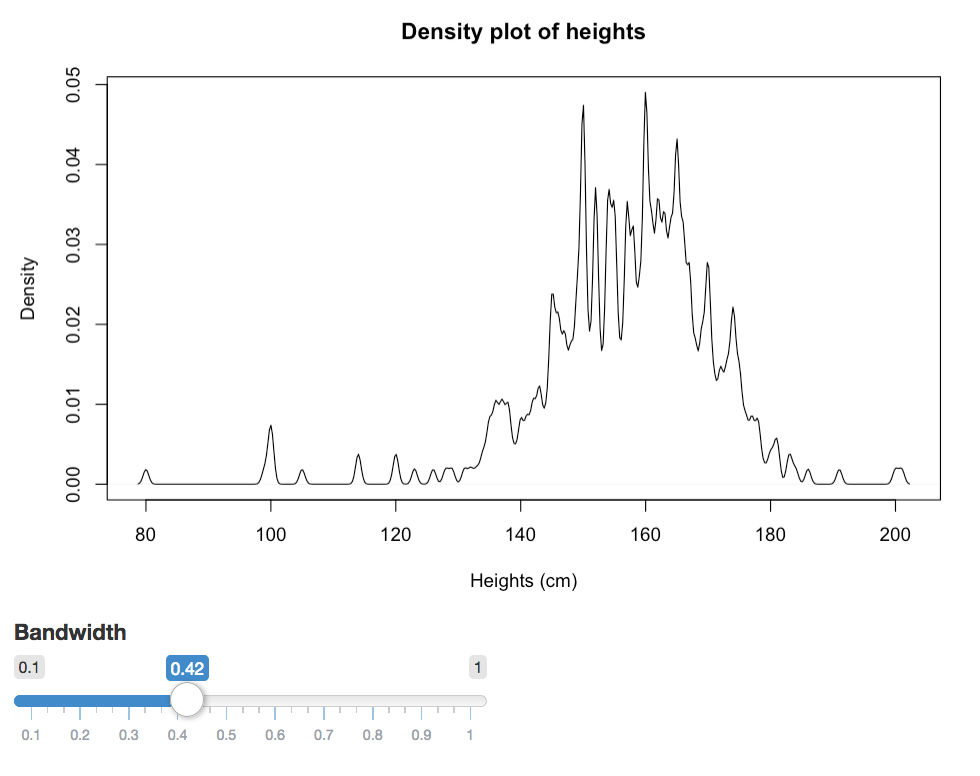
\includegraphics[width=500px,]{./fig/shiny-density} 

}

\caption{\label{fig:d3} control density bandwidth with shiny}\label{fig:unnamed-chunk-94}
\end{figure}

\begin{figure}[H]

{\centering 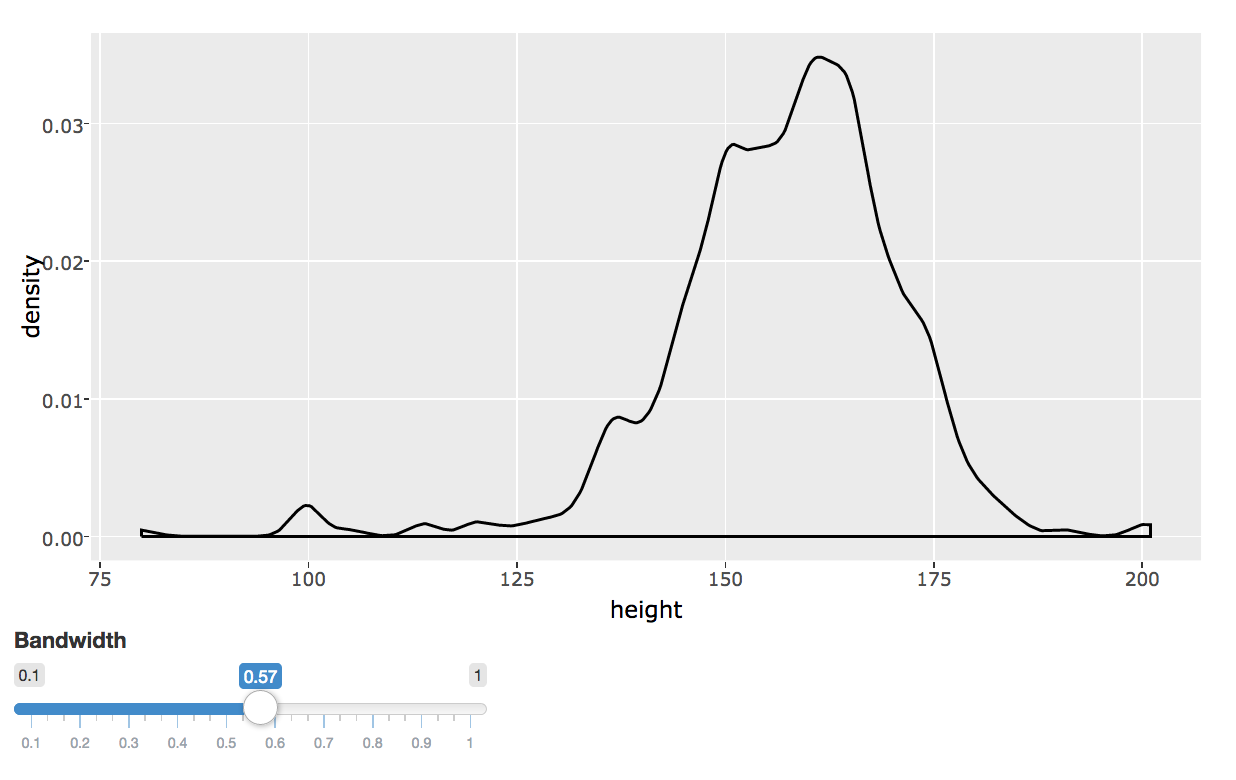
\includegraphics[width=17.17in,]{./fig/ggplotly-density} 

}

\caption{\label{fig:d4} control density bandwidth using plotly (rendered with ggplot2) and shiny}\label{fig:unnamed-chunk-95}
\end{figure}

\begin{longtable}[]{@{}ccccc@{}}
\toprule
\begin{minipage}[b]{0.18\columnwidth}\centering\strut
Tool\strut
\end{minipage} & \begin{minipage}[b]{0.18\columnwidth}\centering\strut
Approximate number of lines of code\strut
\end{minipage} & \begin{minipage}[b]{0.18\columnwidth}\centering\strut
Redraws/reproduces entire plot\strut
\end{minipage} & \begin{minipage}[b]{0.18\columnwidth}\centering\strut
Scale of axes change\strut
\end{minipage} & \begin{minipage}[b]{0.15\columnwidth}\centering\strut
Plot type rendered\strut
\end{minipage}\tabularnewline
\midrule
\endhead
\begin{minipage}[t]{0.18\columnwidth}\centering\strut
interactr (DOM+gridSVG+grid)\strut
\end{minipage} & \begin{minipage}[t]{0.18\columnwidth}\centering\strut
18\strut
\end{minipage} & \begin{minipage}[t]{0.18\columnwidth}\centering\strut
No\strut
\end{minipage} & \begin{minipage}[t]{0.18\columnwidth}\centering\strut
No\strut
\end{minipage} & \begin{minipage}[t]{0.15\columnwidth}\centering\strut
base R\strut
\end{minipage}\tabularnewline
\begin{minipage}[t]{0.18\columnwidth}\centering\strut
ggvis\strut
\end{minipage} & \begin{minipage}[t]{0.18\columnwidth}\centering\strut
3\strut
\end{minipage} & \begin{minipage}[t]{0.18\columnwidth}\centering\strut
No\strut
\end{minipage} & \begin{minipage}[t]{0.18\columnwidth}\centering\strut
Yes\strut
\end{minipage} & \begin{minipage}[t]{0.15\columnwidth}\centering\strut
Vega\strut
\end{minipage}\tabularnewline
\begin{minipage}[t]{0.18\columnwidth}\centering\strut
plotly+shiny\strut
\end{minipage} & \begin{minipage}[t]{0.18\columnwidth}\centering\strut
10\strut
\end{minipage} & \begin{minipage}[t]{0.18\columnwidth}\centering\strut
Yes\strut
\end{minipage} & \begin{minipage}[t]{0.18\columnwidth}\centering\strut
Yes\strut
\end{minipage} & \begin{minipage}[t]{0.15\columnwidth}\centering\strut
ggplot2 (via ggplotly)\strut
\end{minipage}\tabularnewline
\begin{minipage}[t]{0.18\columnwidth}\centering\strut
shiny\strut
\end{minipage} & \begin{minipage}[t]{0.18\columnwidth}\centering\strut
10\strut
\end{minipage} & \begin{minipage}[t]{0.18\columnwidth}\centering\strut
Yes\strut
\end{minipage} & \begin{minipage}[t]{0.18\columnwidth}\centering\strut
Yes\strut
\end{minipage} & \begin{minipage}[t]{0.15\columnwidth}\centering\strut
base R\strut
\end{minipage}\tabularnewline
\bottomrule
\end{longtable}

Table 5.1: A comparison table between existing tools and
\textsf{interactr} on changing the bandwidth of a density plot

From replicating each example, we find that the \textsf{interactr}
package will not change the scale of its axes when the bandwidth is
changed. This is because we are only updating the density line relative
to the coordinates of the axes. In comparison to the rest of the tools,
more lines of code are required to generate the same effect, and those
involving shiny reproduce the entire plot every time.

Because many of these existing tools are still being developed, it is
likely that they will resolve some of the limitations discussed in
Section 2 in the future. However, they require the user to be very
familiar with their APIs. An example of this is the \textsf{plotly}
package that has expanded further into achieving linking between other
types of plots and the ability to prevent redrawing when used with
\textsf{shiny}. It requires the user to know both the plotly API,
\textsf{shiny}, and the \texttt{plotlyProxy()} functions (Sievert 2017a)
as briefly mentioned in Section 2.3.2. The same applies for
\textsf{interactr}. There is still a long way to go before we are
confident enough to claim that users would not need to know
\textsf{DOM}, grid, and \textsf{gridSVG}.

\section{Further problems and future
directions}\label{further-problems-and-future-directions}

The problem of handling large number of individual objects in a plot
remains unresolved as the browser cannot handle too many SVG elements at
once. This is a general problem that occurs across all existing tools. A
solution is to render using webGL and HTML canvas environments which
allow for many elements to be rendered without compromising speed.
However, the problem with this is that it is not as straightforward to
attach events to these elements as they are generally treated as a
single object thus making it difficult to address sub-components.

There is potential in developing \textsf{interactr} further to try
achieve complex interactions that are more useful in exploratory data
analysis. Currently, it is only a proof-of-concept prototype and still
undeveloped in many areas. Only a very small number of examples have
been successful and a limited number of interactions have been
implemented. There is still a need for a simpler and versatile system
for users without compromising the flexibility in which the user can
define interactions and \textsf{interactr} is a step along this path.
Other possible ideas may that may be incorporated include integrating
plots with \textsf{D3} and other htmlwidgets to achieve special effects
such as zooming and panning of a plot and to achieve multi-directional
linking. It may become compatible with \textsf{iNZight} which also uses
the grid system to produce its plots. However, this requires assessment
on how the underlying grid objects are named and drawn before being
implemented.

\section{Conclusion}\label{conclusion}

There is a need in expanding web interactive graphics to create better
data visualisations for users. Despite having many tools available
including plotly, ggvis, shiny and animint and many other packages that
produce htmlwidgets, these generally produce standard interactive plots
outside of R that are hard to customise. interactr provides a way of
driving interactions without the need of learning web technologies while
utilising R's power of statistical computing to aid changes in plots
originally drawn in R. However, more assessment and development is
required on building more informative interactive visualisations before
it can catch up to the capabilities of older desktop applications and
existing tools to be used in the future.

\section{Additional resources}\label{additional-resources}

The \textsf{interactr} package is currently hosted on Github
\href{https://github.com/ysoh286/interactr}{here}.

To install \textsf{interactr}, you need to install DOM v0.4:

\begin{Shaded}
\begin{Highlighting}[]
\KeywordTok{install.packages}\NormalTok{(}\StringTok{"https://github.com/pmur002/DOM/archive/v0.4.tar.gz"}\NormalTok{,}
                \DataTypeTok{repos =} \OtherTok{NULL}\NormalTok{, }\DataTypeTok{type =} \StringTok{"source"}\NormalTok{)}
\NormalTok{devtools}\OperatorTok{::}\KeywordTok{install_github}\NormalTok{(}\StringTok{'ysoh286/interactr'}\NormalTok{)}
\end{Highlighting}
\end{Shaded}

For more details about this project, visit this
\href{https://github.com/ysoh286/honours-project-2017}{repository} which
contains code and additional notes.

\newpage

\chapter*{Bibliography}\label{bibliography}
\addcontentsline{toc}{chapter}{Bibliography}

\hypertarget{refs}{}
\hypertarget{ref-bostock01}{}
Bostock, Michael, Vadim Ogievetsky, and Jeffrey Heer. 2011. ``D3
Data-Driven Documents.'' \emph{IEEE Transactions on Visualization and
Computer Graphics} 17 (12). Piscataway, NJ, USA: IEEE Educational
Activities Department: 2301--9.
doi:\href{https://doi.org/10.1109/TVCG.2011.185}{10.1109/TVCG.2011.185}.

\hypertarget{ref-census01}{}
CensusAtSchool. 2009. \emph{CensusAtSchool 2009 Data Subset}.
\url{http://new.censusatschool.org.nz/resource/2009-censusatschool-data-subset/}.

\hypertarget{ref-ggvis01}{}
Chang, Winston, and Hadley Wickham. 2016. \emph{Ggvis: Interactive
Grammar of Graphics}. \url{https://CRAN.R-project.org/package=ggvis}.

\hypertarget{ref-shiny01}{}
Chang, Winston, Joe Cheng, JJ Allaire, Yihui Xie, and Jonathan
McPherson. 2017. \emph{Shiny: Web Application Framework for R}.
\url{https://CRAN.R-project.org/package=shiny}.

\hypertarget{ref-cheng16}{}
Cheng, Joe. 2016. \emph{Crosstalk: Inter-Widget Interactivity for Html
Widgets}.
\href{https://CRAN.R-project.org/package=crosstalk,\%20https://rstudio.github.io/crosstalk/}{https://CRAN.R-project.org/package=crosstalk, https://rstudio.github.io/crosstalk/}.

\hypertarget{ref-promise02}{}
---------. 2017a. \emph{Async Programming in R and Shiny}.
\url{https://medium.com/@joe.cheng/async-programming-in-r-and-shiny-ebe8c5010790}.

\hypertarget{ref-promise01}{}
---------. 2017b. \emph{Promises: What the Package Does (Title Case)}.

\hypertarget{ref-leaf01}{}
Cheng, Joe, Bhaskar Karambelkar, and Yihui Xie. 2017. \emph{Leaflet:
Create Interactive Web Maps with the Javascript 'Leaflet' Library}.
\url{http://rstudio.github.io/leaflet/}.

\hypertarget{ref-cosway07}{}
Cook, Dianne, and Deborah F. Swayne. 2007. \emph{Interactive and Dynamic
Graphics for Data Analysis - with R and Ggobi}. Use R. Springer.
doi:\href{https://doi.org/10.1007/978-0-387-71762-3}{10.1007/978-0-387-71762-3}.

\hypertarget{ref-crockford01}{}
Crockford, Douglas. 2008. \emph{JavaScript: The Good Parts}. O'Reilly
Media, Inc.

\hypertarget{ref-inz01}{}
Elliott, Tom, and Marco Kuper. 2017. \emph{INZight: INZight Gui for Data
Exploration and Visualisation}.

\hypertarget{ref-gesman01}{}
Gesmann, Markus, and Diego de Castillo. 2011. ``GoogleVis: Interface
Between R and the Google Visualisation Api.'' \emph{The R Journal} 3
(2): 40--44.
\url{https://journal.r-project.org/archive/2011-2/RJournal_2011-2_Gesmann+de~Castillo.pdf}.

\hypertarget{ref-hafen02}{}
Hafen, Ryan. 2016. \emph{Rbokeh Version 0.5.0 Released}.
\url{http://ryanhafen.com/blog/rbokeh-0-5-0}.

\hypertarget{ref-hafen01}{}
Hafen, Ryan, and Inc. Continuum Analytics. 2016. \emph{Rbokeh: R
Interface for Bokeh}. \url{https://CRAN.R-project.org/package=rbokeh}.

\hypertarget{ref-heckmann01}{}
Heckmann, Mark. 2013. \emph{Sending Data from Client to Server and Back
Using Shiny}.
\url{https://ryouready.wordpress.com/2013/11/20/sending-data-from-client-to-server-and-back-using-shiny/}.

\hypertarget{ref-animint01}{}
Hocking, Toby Dylan, Susan VanderPlas, Carson Sievert, Kevin Ferris,
Tony Tsai, and Faizan Khan. 2017. \emph{Animint: Interactive
Animations}. \url{https://github.com/tdhock/animint}.

\hypertarget{ref-ihaka96}{}
Ihaka, Ross, and Robert Gentleman. 1996. ``R: A Language for Data
Analysis and Graphics.'' \emph{Journal of Computational and Graphical
Statistics} 5 (3): 299--314.

\hypertarget{ref-jacobapi01}{}
Jacobson, Daniel, Greg Brail, and Dan Woods. 2011. \emph{APIs: A
Strategy Guide}. O'Reilly Media, Inc.

\hypertarget{ref-kunst01}{}
Kunst, Joshua. 2017. \emph{Highcharter: A Wrapper for the 'Highcharts'
Library}.
\href{https://CRAN.R-project.org/package=highcharter,\%20https://github.com/jbkunst/highcharter}{https://CRAN.R-project.org/package=highcharter, https://github.com/jbkunst/highcharter}.

\hypertarget{ref-murray13}{}
Murray, Scott. 2013. \emph{Interactive Data Visualization for the Web}.
O'Reilly Media, Inc.

\hypertarget{ref-rgraphics01}{}
Murrell, Paul. 2011. \emph{R Graphics}. 2nd ed. Boca Raton, FL, USA: CRC
Press, Inc.

\hypertarget{ref-gridGra01}{}
---------. 2015. \emph{GridGraphics: Redraw Base Graphics Using 'Grid'
Graphics}. \url{https://CRAN.R-project.org/package=gridGraphics}.

\hypertarget{ref-DOM02}{}
---------. 2016a. \emph{An Introduction to the 'Dom' Package}.
\url{https://www.stat.auckland.ac.nz/~paul/Reports/DOM/Intro/DOM-Intro.html}.

\hypertarget{ref-DOM01}{}
---------. 2016b. \emph{DOM: Interact with Web Browser Dom}.

\hypertarget{ref-gridSVG03}{}
Murrell, Paul, and Simon Potter. 2012. \emph{Working with the gridSVG
Coordinate System}.
\url{https://www.stat.auckland.ac.nz/~paul/Reports/gridSVGcoords/coordinates.html}.

\hypertarget{ref-gridSVG02}{}
---------. 2014. ``The gridSVG Package.'' \emph{R Journal} 6 (1):
133--43.
\url{https://journal.r-project.org/archive/2014/RJ-2014-013/RJ-2014-013.pdf}.

\hypertarget{ref-gridSVG01}{}
---------. 2017. \emph{GridSVG: Export 'Grid' Graphics as Svg}.
\url{https://CRAN.R-project.org/package=gridSVG}.

\hypertarget{ref-record01}{}
Paul Murrell, Jeroen Ooms, and JJ Allaire. 2015. \emph{Recording and
Replaying the Graphics Engine Display List}.
\url{https://www.stat.auckland.ac.nz/~paul/Reports/DisplayList/dl-record.html}.

\hypertarget{ref-shiny03}{}
RStudio. 2017a. \emph{Interactive Plots}.
\href{https://shiny.rstudio.com/articles/plot-interaction.html,\%20https://shiny.rstudio.com/articles/plot-interaction-advanced.html}{https://shiny.rstudio.com/articles/plot-interaction.html, https://shiny.rstudio.com/articles/plot-interaction-advanced.html}.

\hypertarget{ref-shiny05}{}
---------. 2017b. \emph{Selecting Rows of Data}.
\url{https://shiny.rstudio.com/articles/selecting-rows-of-data.html}.

\hypertarget{ref-shiny02}{}
---------. 2017c. \emph{Shiny}. \url{https://shiny.rstudio.com/}.

\hypertarget{ref-shiny04}{}
---------. 2017d. \emph{Shiny Server}.
\url{https://www.rstudio.com/products/shiny/shiny-server/}.

\hypertarget{ref-sievert03}{}
Sievert, Carson. 2017a. \emph{Plotly 4.7.1 Now on Cran}.
\url{http://moderndata.plot.ly/plotly-4-7-1-now-on-cran/}.

\hypertarget{ref-sievert01}{}
---------. 2017b. \emph{Plotly for R}.
\url{https://plotly-book.cpsievert.me/}.

\hypertarget{ref-plotly01}{}
Sievert, Carson, Chris Parmer, Toby Hocking, Scott Chamberlain, Karthik
Ram, Marianne Co rvellec, and Pedro Despouy. n.d. \emph{Plotly: Create
Interactive Web Graphics via 'Plotly.js'}.
\href{https://plot.ly/r,\%20https://cpsievert.github.io/plotly_book/,\%20https://github.com/ropensci/plotly}{https://plot.ly/r, https://cpsievert.github.io/plotly\_book/, https://github.com/ropensci/plotly}.

\hypertarget{ref-theus02}{}
Theus, Martin. 2002. ``Interactive Data Visualization Using Mondrian.''
\emph{Journal of Statistical Software, Articles} 7 (11): 1--9.
doi:\href{https://doi.org/10.18637/jss.v007.i11}{10.18637/jss.v007.i11}.

\hypertarget{ref-vega01}{}
Trifacta. 2014. \emph{Vega}. \url{https://vega.github.io/vega/}.

\hypertarget{ref-unwin01}{}
Unwin, Antony, Martin Theus, and Heike Hofmann. 2006. \emph{Graphics of
Large Datasets: Visualizing a Million (Statistics and Computing)}.
Secaucus, NJ, USA: Springer-Verlag New York, Inc.

\hypertarget{ref-iplot01}{}
Urbanek, Simon, and Tobias Wichtrey. 2013. \emph{Iplots: IPlots -
Interactive Graphics for R}.
\url{https://CRAN.R-project.org/package=iplots}.

\hypertarget{ref-vaidyan13}{}
Vaidyanathan, Ramnath. 2013. \emph{RCharts: Interactive Charts Using
Javascript Visualization Libraries}.

\hypertarget{ref-w3c}{}
W3C. 2009. \emph{Document Object Model (Dom)}.
\url{https://www.w3.org/DOM/}.

\hypertarget{ref-w3c02}{}
---------. 2016. \emph{HTML \& Css}.
\url{https://www.w3.org/standards/webdesign/htmlcss}.

\hypertarget{ref-ggplot01}{}
Wickham, Hadley. 2009. \emph{Ggplot2: Elegant Graphics for Data
Analysis}. Springer-Verlag New York. \url{http://ggplot2.org}.

\hypertarget{ref-wickham01}{}
---------. 2016. \emph{Ggplot2: Elegant Graphics for Data Analysis}.
Springer-Verlag New York. \url{http://ggplot2.org}.

\hypertarget{ref-ggvis02}{}
Wickham, Hadley, and Winston Chang. 2016. \emph{Interactivity}.
\url{http://ggvis.rstudio.com/interactivity.html}.

\hypertarget{ref-wilkin01}{}
Wilkinson, Leland. 2005. \emph{The Grammar of Graphics (Statistics and
Computing)}. Secaucus, NJ, USA: Springer-Verlag New York, Inc.

\hypertarget{ref-dt01}{}
Xie, Yihui. 2016. \emph{DT: A Wrapper of the Javascript Library
'Datatables'}. \url{http://rstudio.github.io/DT}.


\end{document}
